% CVPR 2024 Paper Template; see https://github.com/cvpr-org/author-kit

\documentclass[runningheads]{llncs}

% ---------------------------------------------------------------
% Include basic ECCV package
 
% TODO REVIEW: Insert your submission number below by replacing '*****'
% TODO FINAL: Comment out the following line for the camera-ready version
% \usepackage[review,year=2024,ID=5548]{eccv}
% TODO FINAL: Un-comment the following line for the camera-ready version
\usepackage{eccv}

% OPTIONAL: Un-comment the following line for a version which is easier to read
% on small portrait-orientation screens (e.g., mobile phones, or beside other windows)
%\usepackage[mobile]{eccv}


% ---------------------------------------------------------------
% Other packages

% Commonly used abbreviations (\eg, \ie, \etc, \cf, \etal, etc.)
\usepackage{eccvabbrv}

% Include other packages here, before hyperref.
\usepackage{graphicx}
\usepackage{booktabs}

\usepackage{multirow}
\usepackage{makecell}
\usepackage{wrapfig}
\usepackage{xcolor} 
\usepackage{pifont}
% The "axessiblity" package can be found at: https://ctan.org/pkg/axessibility?lang=en
\usepackage[accsupp]{axessibility}  % Improves PDF readability for those with disabilities.

\usepackage{booktabs}
\usepackage{multicol}
\usepackage{colortbl}
\usepackage{multirow}
% \usepackage{amsthm}
% \newtheorem{theorem}{Theorem} 
% \newtheorem{lemma}{Lemma} 
% \newtheorem{remark}{Remark}
\usepackage{amssymb}
% \usepackage{pifont}
\usepackage{comment}
\usepackage[normalem]{ulem}
\usepackage{xcolor}


% It is strongly recommended to use hyperref, especially for the review version.
% hyperref with option pagebackref eases the reviewers' job.
% Please disable hyperref *only* if you encounter grave issues, 
% e.g. with the file validation for the camera-ready version.
%
% If you comment hyperref and then uncomment it, you should delete *.aux before re-running LaTeX.
% (Or just hit 'q' on the first LaTeX run, let it finish, and you should be clear).
\definecolor{cvprblue}{rgb}{0.21,0.49,0.74}
\usepackage[pagebackref,breaklinks,colorlinks,citecolor=cvprblue]{hyperref}

%%%%%%%%% PAPER ID  - PLEASE UPDATE


%%%%%%%%% TITLE - PLEASE UPDATE
\title{DGR-MIL: Exploring Diverse Global Representation in Multiple Instance Learning for Whole Slide Image Classification}

\titlerunning{DGR-MIL}
%%%%%%%%% AUTHORS - PLEASE UPDATE
% \author{Wenhui Zhu\\
% Institution1\\
% Institution1 address\\
% {\tt\small firstauthor@i1.org}
% % For a paper whose authors are all at the same institution,
% % omit the following lines up until the closing ``}''.
% % Additional authors and addresses can be added with ``\and'',
% % just like the second author.
% % To save space, use either the email address or home page, not both
% \and
% Second Author\\
% Institution2\\
% First line of institution2 address\\
% {\tt\small secondauthor@i2.org}
% }

\def\thefootnote{*}\footnotetext{These authors contributed equally to this paper.}
\def\thefootnote{$\dagger$}\footnotetext{Corresponding author}

\author{Wenhui Zhu\inst{1* \dagger} \and
Xiwen Chen\inst{2*} \and
Peijie Qiu\inst{3*}  \and \\
Aristeidis Sotiras\inst{3} \and Abolfazl Razi\inst{2} \and Yalin Wang\inst{1} \\
}
%
\authorrunning{Zhu. Wenhui et al.}
% First names are abbreviated in the running head.
% If there are more than two authors, 'et al.' is used.
%
\institute{ Arizona State University, AZ, USA \\ {\tt\small \{wzhu59,ylwang\}@asu.edu} \and
Clemson University, SC, USA \\ {\tt\small xiwenc@g.clemson.edu, arazi@clemson.edu} \and
Washington University in St. Louis, MO, USA \\
{\tt\small \{peijie.qiu,aristeidis.sotiras\}@wustl.edu }
}

\begin{document}
\maketitle
% \begin{abstract}
 Current monocular 3D scene reconstruction (3DR) works are either fully-supervised, or not generalizable, or implicit in 3D representation. We propose a novel framework - \textbf{MonoSelfRecon} that for the first time achieves \textbf{explicit 3D mesh} reconstruction for \textbf{generalizable} indoor scenes with monocular RGB views by purely \textbf{self-supervision} on voxel-SDF (signed distance function). MonoSelfRecon follows an Autoencoder-based architecture, decodes voxel-SDF and a generalizable Neural Radiance Field (NeRF), which is used to guide voxel-SDF in self-supervision. We propose novel self-supervised losses, which not only support pure self-supervision, but can be used together with supervised signals to further boost supervised training. Our experiments show that "MonoSelfRecon" trained in pure self-supervision outperforms current best self-supervised indoor depth estimation models and is comparable to 3DR models trained in fully supervision with depth annotations. MonoSelfRecon is not restricted by specific model design, which can be used to any models with voxel-SDF for purely self-supervised manner. %\footnote{Datasets  were  downloaded  and  evaluated  solely  by  the researchers from UC San Diego.}
\end{abstract}    
% \section{Introduction} \label{intro}


With the recent development of deep generative models, speech synthesis has seen an extraordinary progress. Among the conventional speech synthesis methods, WaveNets~\cite{oord2016wavenet} were demonstrated to generate high-fidelity audio samples in an autoregressive manner yet suffering from prohibitively expensive computational costs. In contrast, non-autoregressive approaches such as flow-based and GAN-based models~\cite{prenger2019waveglow,jang2021univnet,kong2020hifi,huang2021multi} were also proposed to generate speech audios with satisfactory speed. However, these models were still criticized for other problems, e.g., the limited sample quality or sample diversity \cite{xiao2021tackling}.

In speech synthesis, our goal is mainly two-fold:
\begin{itemize}
    \item High-quality: generating high-quality speech is a challenging problem especially when the sampling rate of an audio is high. It is vital to reconstruct details at different timescales for waveforms of highly variable patterns.
    \item Fast: high generation speed is essential when considering real-time speech synthesis. This poses a challenge for all high-quality neural synthesizers.
\end{itemize}

As a blossoming class of generative models, denoising diffusion probabilistic models (DDPMs)~\cite{ho2020denoising,song2020denoising,lam2022bddm,liu2022pseudo} has emerged to prove its capability to achieve leading performances in both image and audio syntheses~\cite{dhariwal2021diffusion,san2021noise,kong2020diffwave,chen2020wavegrad,lam2022bddm}. However, current development of DDPMs in speech synthesis was hampered by two major challenges:
\begin{itemize}
\item Different from other existing generative models, diffusion models are not trained to directly minimize the difference between the generated audio and the reference audio, but to de-noise a noisy sample given an optimal gradient. This in practice could lead to overly de-noised speech after a large number of sampling steps, in which natural voice characteristics including breathiness and vocal fold closure are removed.
\item While DDPMs inherently are gradient-based models, a guarantee of high sample quality typically comes at a cost of hundreds to thousands of de-noising steps. When reducing the sampling steps, an apparent degradation in quality due to perceivable background noise is observed.
\end{itemize}

In this work, we propose FastDiff, a fast conditional diffusion model for high-quality speech synthesis. To improve audio quality, FastDiff adopts a stack of time-aware location-variable convolutions of diverse receptive field patterns to efficiently model long-term time dependencies with adaptive conditions. To accelerate the inference procedure, FastDiff also includes a noise schedule predictor, which derives a short and effective noise schedule and significantly reduces the de-noising steps. Based on FastDiff, we also introduce an end-to-end phoneme-to-waveform synthesizer FastDiff-TTS, which simplifies the text-to-speech generation pipeline and does not require intermediate features or specialized loss functions to enjoy low inference latency.

Experimental results demonstrated that FastDiff achieved a higher MOS score than the best publicly available models and outperformed the strong WaveNet vocoder (MOS: 4.28 vs. 4.20). FastDiff further enjoys an effective sampling process and only needs 4 iterations to synthesize high-fidelity speech, 58x faster than real-time on a V100 GPU without engineered kernels. To the best of our knowledge, FastDiff is the first diffusion model with a sampling speed comparable to previous  for the first time applicable to interactive, real-world speech synthesis applications at a low computational cost. FastDiff-TTS successfully simplify the text-to-speech generation pipeline and outperform competing architectures.
% \input{sec/2_formatting}
% \input{sec/3_finalcopy}
% \input{sec/4_ablation}


\begin{abstract}
Multiple instance learning (MIL) stands as a powerful approach in weakly supervised learning, regularly employed in histological whole slide image (WSI) classification for detecting tumorous lesions. However, existing mainstream MIL methods focus on modeling correlation between instances while overlooking the inherent diversity among instances. However, few MIL methods have aimed at diversity modeling, which empirically show inferior performance but with a high computational cost.
To bridge this gap, we propose a novel MIL aggregation method based on diverse global representation (DGR-MIL), by modeling diversity among instances through a set of global vectors that serve as a summary of all instances. First, we turn the instance correlation into the similarity between instance embeddings and the predefined global vectors through a cross-attention mechanism. This stems from the fact that similar instance embeddings typically would result in a higher correlation with a certain global vector. Second, we propose two mechanisms to enforce the diversity among the global vectors to be more descriptive of the entire bag: (i) positive instance alignment and (ii) a novel, efficient, and theoretically guaranteed diversification learning paradigm. Specifically, the positive instance alignment module encourages the global vectors to align with the center of positive instances (e.g., instances containing tumors in WSI). To further diversify the global representations, we propose a novel diversification learning paradigm leveraging the determinantal point process. The proposed model outperforms the state-of-the-art MIL aggregation models by a substantial margin on the CAMELYON-16 and the TCGA-lung cancer datasets. The code is available at \url{https://github.com/ChongQingNoSubway/DGR-MIL}.
% \vspace{-0.3cm}
\begin{figure}[!t]
    \centering
    \includegraphics[width=1.0\columnwidth]{Figure/diversity_vis.jpg}
    \caption{(a) Examples of positive instances of with-bag and between-bag diversities measured by rate-distortion theory. (b) Histogram of the diversity measure within positive bags on the CAMELYON16 dataset. (c) The between-bag distinction measures the pair-wise similarity between bags.}  %The between-bag distinction measures the between-bag diversity among positive bags.
    \vspace{-0.4cm}
    \label{fig:div_vis}
\end{figure}
  \keywords{Weakly-supervised learning, Multiple Instance Learning \and Histological Whole Slide Image \and Transformer}
\end{abstract}

\section{Introduction}
Histological whole slide images (WSIs) are commonly used to diagnose a variety of cancers, e.g., breast cancer, lung cancer, etc.~\cite{cancer}. However, the gigapixel resolution of WSIs hinders the direct translation of classic deep learning methods into WSI applications mainly due to computational intractability~\cite{wsi1,wsi2,wsi3,clam-sb}. Therefore, the analysis of WSIs typically starts with cropping images into small patches and then performing analysis on a per-patch basis. In addition, the absence of labor-intensive pixel/patch-level annotations poses a significant challenge for the precise localization of targets of interest (e.g., tumors in WSIs) in a fully supervised setting. As a result, Multiple Instance Learning (MIL), a weakly supervised method, is commonly employed in WSI analyses by treating an entire WSI as a bag and the cropped patches as instances. \\
\indent The prevailing MIL models in analyzing WSIs have been built upon the attention-based MIL (AB-MIL) framework ~\cite{ilse2018attention} since its introduction. However, the standard AB-MIL treats each instance independently and does not take the correlations between instances into account. Although many of its follow-ups address this challenge by a variety of means~\cite{li2021dual,shao2021transmil,zhang2022dtfd,lowrankmil}, they mainly focus on modeling the correlation between instances by assigning high correlations to instances from the same category (e.g., tumor instances). However, even instances from the same category exhibit variations in phenotype, size, as well as spatial diversity marked by immune infiltration across different patients~\cite{clinicdiversity,clinicdiversity2,clinicdiversity3}. For example, negative instances close to the tumor boundaries typically resemble positive instances while appearing differently compared to the other negative instances~\cite{similaritysupport}. As a result, instances belonging to the same category may not be assigned high correlations; similarly, instances from different categories could also receive high correlations. This spurious correlation between instances is prone to trap the MIL model by incorrectly aggregating them when making predictions. Formally, we quantify the diversity of instances between and within bags in WSIs by leveraging the rate-distortion theory~\cite{cover1999elements,yu2020learning,chen2023rd}, where a higher rate indicates a less compressible but more diverse collection of samples (see details of computing the diversity measure in Appendix A). As consistent with findings in pathology, we observe that both positive and negative instances in WSIs exhibit between-bag and within-bag diversity (refer to Fig.  \ref{fig:div_vis}). Based on this fact, we argue that the diversity of instances is important in designing MIL models. Before that, clustering/prototype-based MIL methods tried to solve the diversity by utilizing attention scores as pseudo labels to provide instance-level supervision~\cite{tpmil,scmil}. This introduces a chicken-and-egg issue. The effectiveness of pseudo-labels relies on successful MIL classification pooling, which in turn depends on precise attention localization. Especially when patch representations are inferior or MIL initially guided by poor pseudo label, leading to even misleading localization and unstable optimization~\cite{iterself,PDL}. Among them, PMIL presents an alternative method to avoiding noise attention~\cite{pmil}, initially selecting prototypes through clustering, followed by modeling diversity via prototype and patch representation. However, the design of the multi-stage framework empirically leads to suboptimal learning outcomes, and the restricted number of prototypes, due to high computational burden, results in diminished diversity. \\
\indent To this end, we propose to jointly model this diversity through a set of learnable global vectors. The learned global vectors summarize diverse instances of interest (e.g., tumors in WSIs). As a result, the diversity between instances can be implicitly modeled by computing the correlation between instance embeddings and the global vectors through a cross-attention mechanism. To enhance the ability of the global vectors to capture the most discriminative global context for WSI classification, we introduce the concept of tokenized global vectors. It is worth mentioning that the importance map for instances can be calculated based on the attention between the tokenized global vector and the embedding of each individual instance. To learn diverse global vectors, we propose two main strategies. First, we push the global vectors toward the centers of the positive bag by a positive instance alignment mechanism. Second, we propose a low-complexity and theoretically guaranteed diversity loss to enforce the orthogonality between the global vectors by utilizing the linear algebra property of the determinantal point process (DPP). In this paper, we explore the design of diverse global representation in the MIL model to model the diversity of instances in WSI. The main contributions are four-fold: (i) We introduce a new perspective on modeling the diversity of instances in WSI. (ii) We further propose a novel MIL aggregation model, termed DGR-MIL, to model diversity in MIL through a set of learnable global vectors. (iii) To learn a diverse global representation (vectors), we propose two main mechanisms: positive instance alignment and a novel diversity loss. 
(iv) Experimental results on two WSI benchmarks demonstrate the proposed DGR-MIL outperforms other competing MIL aggregation methods.



% \vspace{-0.4cm}
\section{Related Work}
\subsection{Multiple instance learning in WSIs}
MIL has been widely applied in many fields, e.g., pathology~\cite{ilse2018attention,li2021dual,shao2021transmil,zhang2022dtfd}, video analysis~\cite{babenko2010robust,quellec2017multiple}, time series~\cite{early2024inherently,chen2024timemil}.
In particular, the applications of the MIL in Whole Slide Image classification can be roughly summarized into two sub-categories: i) instance-based MIL~\cite{feng2017deep, hou2016patch, xu2019camel} and ii) bag embedding-based MIL. Instance-based methods typically require the propagation of the bag-level label to each of its instances to train the model. Consequently, the final bag-level prediction is obtained by aggregating instance-level predictions. However, empirical studies have proven its performance inferior to the embedding-based competitors because of the noisy instance-level supervision~\cite{wang2018revisiting}. In contrast, bag-embedding-based methods start by projecting instances into feature embeddings and subsequently aggregate the information of these embeddings to obtain the bag-level prediction. Since the introduction of attention-based MIL (AB-MIL)~\cite{ilse2018attention}, the prevailing applications of bag embedding-based MIL in WSI analysis have revolved around this framework. However, AB-MIL operates under the assumption that all instances within a bag are independent and identically distributed while failing to uncover inter-instance correlations. Therefore, numerous of its follow-up works centered around mitigating this limitation by taking advantage of non-local attention mechanism~\cite{li2021dual}, transformer~\cite{shao2021transmil}, pseudo bags~\cite{zhang2022dtfd}, sparse coding~\cite{qiu2023sc}, and low-rank constraints~\cite{lowrankmil}. 

Most existing mainstream MIL methods have modeled correlations mainly through similarity between instances. However, they did not consider the variability of instances between and within bags. Conversely, clustering/prototype-based MIL employs attention scores for selecting prototypes~\cite{scmil,tpmil}, potentially introducing noise and misleading model decisions~\cite{PDL,iterself}. Unlike attention-guided methods, PMIL \cite{pmil} suggests a two-stage framework that first leverages clustering to identify reference prototypes and capture the sub-cluster representation among patch instances and prototypes. However, unrestricted optimization in prototype selection can easily lead to suboptimal outcomes, and a limited number of prototypes can result in a loss of diversity (limited by computational resources).
In this paper, we explicitly model the diversity among instances in bag-embedding-based MIL through a learnable global representation. Although the proposed method falls into the category of transformer-based MILs, it differs from the previous transformer-based MILs~\cite{shao2021transmil, lowrankmil} in two main aspects. First, we model the diversity between instances by comparing instances to the proposed global vectors via a cross-attention mechanism.
Second, we propose a tokenized global vector to summarize the context information of positive instances. 

\subsection{Transformer}
 The transformer~\cite{attentionisallyouneed} has been widely applied in computer vision~\cite{vit,swimtransformer,crossattention2,carion2020end}, time series modeling~\cite{timeserise1,timeserise2}, and the natural language processing fields~\cite{nlp1,nlp2,nlp3}. Standard transformers discover contextually relevant information by modeling the correlation between elements within a sequence through the self-attention mechanism. However, the traditional self-attention operation has quadratic time and space complexity $\mathcal{O}(n^2)$, with respect to a sequence containing $n$ elements. In the context of MIL, sequence length typically becomes quite large since one bag often approximately comprises ten thousand instances. This extremely long sequence poses significant computational intractability. Although \cite{wang2020linformer,shen2021efficient,guo2022beyond} demonstrate that proper approximation of standard self-attention can reduce its quadratic complexity to linear, it still struggles to capture extremely long-term dependencies of context \cite{bhattamishra2020computational,ruoss2023randomized,lowrankmil}.
In contrast, the cross-attention mechanism~\cite{crossattention2,crossattention3}, which was originally proposed to relate positions from one sequence to another, allows models to consider cross-sequence information. Inspired by this, we 
propose to model the diversity between and among instances through a cross-attention between instances and the proposed global vectors (see details in Section~\ref{sec:grmp}). This dramatically reduces the complexity compared to the self-attention mechanism (see Appendix C for details of model complexity) since the number of global vectors is significantly less than the sequence length.

\begin{figure*}[t]
\centering
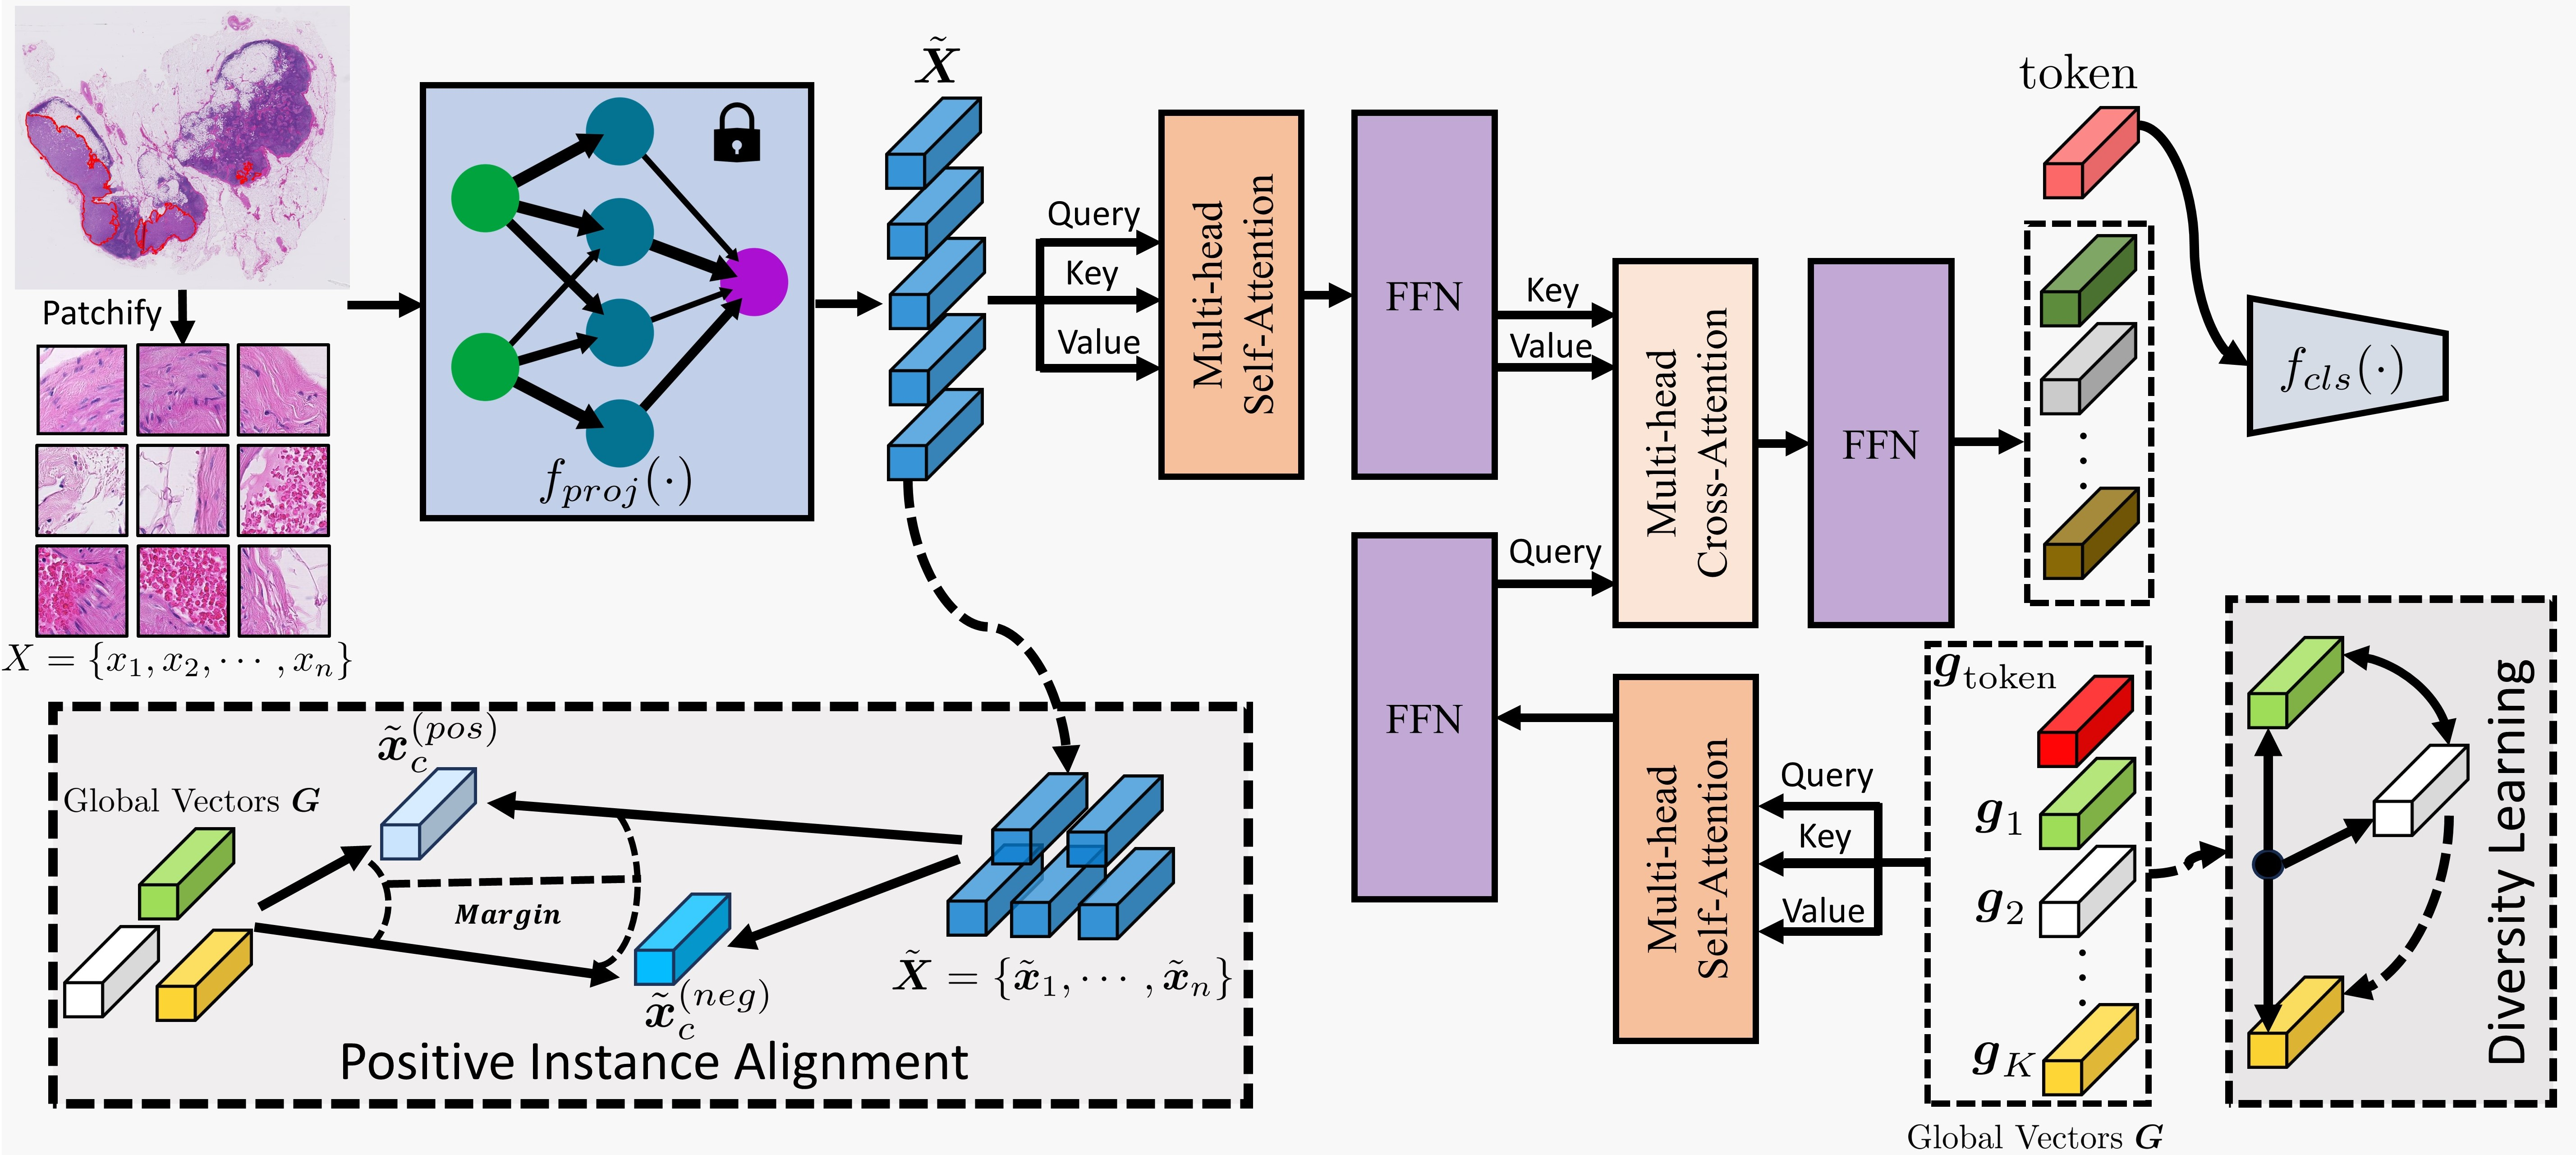
\includegraphics[width=1.0\textwidth]{Figure/network.jpg} % Reduce the figure size to slightly narrower than the column.
\caption{Overview of the proposed DGR-MIL where the global vectors are used for modeling the diversity of instances. The diverse global vectors are learned through the positive instance alignment module and the diversity learning mechanism.}
\label{fig:workflow}
\end{figure*}

\section{Methods}
The proposed DGR-MIL comprises two main parts: i) the design of the global representation in MIL pooling (Section~\ref{sec:grmp}), and ii) the strategy of learning diverse global representation (Section~\ref{sec:GRCL}), where we further propose positive instance alignment and a computational-efficient diversity loss with a theoretical guarantee. The entire framework of DGR-MIL is depicted in Fig. \ref{fig:workflow}.

% \subsection{Preliminary}
%  Take the binary MIL classification as an example:
\noindent \textbf{Preliminary.} Without loss of generality, we take binary MIL classification as an example:
The objective is to predict the bag-level label $Y \in \{0, 1\}$, given a bag of instances $\boldsymbol{X} = \{\boldsymbol{x}_1, \boldsymbol{x}_2, \cdots, \boldsymbol{x}_n\}$, denoting a WSI with $n$ tiled patches. However, the corresponding instance-level labels $\{y_i\}_{i=1}^{n}$ are unknown in most WSI analyses due to the laboriousness of obtaining patch-level annotations. This turns the WSI classification into a weakly-supervised learning scheme according to the standard MIL formulation: 
\begin{equation}
    Y = \begin{cases}
     0, \ \text{iff} \ \sum_{i} y_i = 0 \\
     1, \ \text{otherwise}.
    \end{cases}
\end{equation}
Because of the gigapixel resolution of WSIs, MIL typically cannot be performed in an end-to-end fashion~\cite{clam-sb,end2endsupport,end2endsupport2} and instead necessitates a simplified learning scheme. This simplified MIL learning process comprises three main parts: i) a pre-trained feature extractor $f_{proj}(\cdot)$ that projects each instance into a $L$-dimensional vector, ii) a MIL pooling operator $\sigma(\cdot)$ that combines instance-level embeddings into a bag-level feature, and iii) a bag-level classifier $f_{cls}(\cdot)$ that takes the bag-level feature as input and produces the bag-level prediction as output. Mathematically, this process is given by
\begin{equation}
\begin{split}
     & \ \ \ \ \hat{Y} = f_{cls}(\sigma(\{\Tilde{\boldsymbol{x}}_1, \cdots, \Tilde{\boldsymbol{x}}_n\})), \ \Tilde{\boldsymbol{x}}_i \in \mathbb{R}^{L} \\
     & \text{with} \ \{\Tilde{\boldsymbol{x}}_1, \cdots, \Tilde{\boldsymbol{x}}_n\} = f_{proj}(\{\boldsymbol{x}_1, \cdots, \boldsymbol{x}_n\}),
      % \text{with}\quad&\Tilde{\boldsymbol{x}}_i = f_{proj}(\{\boldsymbol{x}_i),
\end{split}
\end{equation}
where $\hat{Y}$ denotes the predicted bag-level label.
In the attention-based MIL (AB-MIL) \cite{ilse2018attention} framework, the typical formulation for the MIL pooling operator is as follows:
\begin{equation}
    \sigma(\Tilde{\boldsymbol{x}}_i) = \frac{\exp\{\boldsymbol{W}^\mathrm{T} (\text{tanh}(\boldsymbol{V} \Tilde{\boldsymbol{x}}_i)) \odot \text{sigm}(\boldsymbol{U}\Tilde{\boldsymbol{x}}_i) \}}{\sum_{i=1}^{n} \exp\{\boldsymbol{W}^\mathrm{T} (\text{tanh}(\boldsymbol{V} \Tilde{\boldsymbol{x}}_i)) \odot \text{sigm}(\boldsymbol{U}\Tilde{\boldsymbol{x}}_i) \}},
\label{eqn:abmil}
\end{equation}
where $\boldsymbol{W}, \boldsymbol{V}$, and $\boldsymbol{U}$ are learnable parameters. 

\subsection{Global Representation in MIL Pooling}
\label{sec:grmp}

To accommodate the variability of the target lesions within and between bags, we develop a diverse global representation in the MIL pooling stage. Specifically, we define the global representation of the target (positive) instances as a set of learnable vectors given by 
% $\boldsymbol{G} = \{\boldsymbol{g}_1, \cdots, \boldsymbol{g}_K \}$
$\boldsymbol{G} = [\boldsymbol{g}_1^\top, \cdots, \boldsymbol{g}_K^\top ]\in \mathbb{R}^{K \times L}$
with $\boldsymbol{g}_k \in \mathbb{R}^{L}$ where $K$ is the number of global vectors. It is worth noting that a feed-forward network (FFN) is used to embed further both the input instance vectors $\Tilde{\boldsymbol{X}}=\{\Tilde{\boldsymbol{x}}_i\}_{i=1}^{n}$ and the global vectors $\boldsymbol{G}$ (see Fig. \ref{fig:workflow}). However, we keep using $\boldsymbol{G}\in \mathbb{R}^{K \times L}$ to denote global vectors for notation brevity.   

% To capture the global representation of positive instances, we defined a learnable parameter $G \in \mathbb{R}^{K \times H}$ as the global representation. The $K$ is the number of global representation instances, and $H$ is the embedding feature dimension. The $N$ extracted patches project to instance features $I \in \mathbb{R}^{N \times H}$ after through the instance projector. We feed $I$ and $G$ to a multilayer perceptron layer (MLP) for reducing dimension to $L$, which obtained $G \in \mathbb{R}^{K \times L}$, $I \in \mathbb{R}^{N \times L}$ respectively. 

\subsubsection{Instance Correlation as Cross Attention.} The standard AB-MIL framework assumes the instances are independent and identically distributed while overlooking the correlation effect between instances. Hence, the self-attention mechanism becomes a natural choice for modeling the inter-instance correlation. However, due to the large number of instances within a bag in MIL, the quadratic time and space complexity $\mathcal{O}(n^2)$ of standard self-attention poses a significant challenge in computation. Alternatively, the previous transformer-based MIL~\cite{shao2021transmil} mitigates this problem by employing Nystrom-Attention~\cite{xiong2021nystromformer}, approximating the standard self-attention with linear complexity, which has proved effective of modeling correlation between positive and negative instances. It could be used to gather similar instances together by attention, benefiting from filtering background information. However, self-attention usage only guarantees the general separation of the positive and negative instances in a bag, which overlooks the diversity between instances and between bags. 

Here, we implicitly model the diversity between instances by comparing the similarity between each instance vector and the proposed diverse global vectors. Specifically, this is achieved through a cross-attention mechanism where the global vector $\boldsymbol{G}$ serves as queries, and a bag of instance vectors $\Tilde{\boldsymbol{X}}$ is used as key-value pairs. Formally, the $h$-th head of the proposed cross attention is given by
\begin{equation}
\begin{split}
    &  \ \ \ \ \ \text{head}_h(\boldsymbol{G}, \Tilde{\boldsymbol{X}}) = \operatorname{Attention}(\boldsymbol{Q}_h, \boldsymbol{K}_h, \boldsymbol{V}_h) \\
    & \boldsymbol{Q}_h = \boldsymbol{G} \boldsymbol{W}_h^{Q}, \ \ \ \boldsymbol{K}_h = \Tilde{\boldsymbol{X}} \boldsymbol{W}_h^{K}, \ \ \ \boldsymbol{V}_h = \Tilde{\boldsymbol{X}} \boldsymbol{W}_h^{V} ,
\end{split}
\end{equation}
where $\boldsymbol{W}^{Q}_h$, $\boldsymbol{W}^{K}_h$, $\boldsymbol{W}^{V}_h \in \mathbb{R}^{L \times L/H}$ are learnable parameters for linear projections, where $H$ is number of heads. For the derivation purposes, we follow the traditional definition of the attention mechanism in the transformer (i.e., $\operatorname{Attention}(\boldsymbol{Q}_h, \boldsymbol{K}_h, \boldsymbol{V}_h) = \operatorname{softmax}\left( \boldsymbol{Q}_h \boldsymbol{K}_h^{\top} / \sqrt{d_k} \right) \boldsymbol{V}_h$). The output of the yielding multi-head cross attention (MHCA) is the concatenation of the outputs from all heads through a linear projection: 
\begin{equation}
    \text{MHCA}(\boldsymbol{G}, \Tilde{\boldsymbol{X}}) = \operatorname{concat}(\text{head}_1; \cdots; \text{head}_H)\boldsymbol{W}^{O},
\label{eqn:mhca}
\end{equation}
where $\boldsymbol{W}^{O} \in \mathbb{R}^{L \times L}$ is a trainable parameter. The proposed cross-attention mechanism reduces the quadratic time and space complexity $\mathcal{O}(n^2)$ in the standard self-attention mechanism to linear $\mathcal{O}(Kn)$ where $K \ll n$. In practice, we applied the Nystrom-Attention to the instance vectors and global vectors before performing the cross-attention (see Fig. \ref{fig:workflow}) for two main reasons. First, applying self-attention to input instance vectors can facilitate filtering out the background. Second, applying self-attention to the global vectors can increase their discrepancies. 

% In WSI, notwithstanding the application of preprocessing to extract patches~\cite{clam-sb,li2021dual}, the presence of instances with background information persists. Moreover, medical experts typically took into consideration contiguous regions to diagnose, primarily due to the positive patches having shared tumor morphologies~\cite{sharedtumor}. The self-attention is a good choice to build the correlation between instances by querying the similarity. Similar to the \cite{shao2021transmil}, we utilized the multi-head self-attention (MSA) to filter the background and enhance the lesion instances. It is worth noting that we did not use the position encoding. The MSA can be represented as 
% \begin{align}
% \begin{split}
%     MSA(Q,K,V)= Concat(head_{1},...,head_{h})W^{O}\\
%     where \ \ head_{h} = Attention(QW_{h}^{Q},KW_{h}^{K},VW_{h}^{V})
% \end{split}
% \label{Eq:MSA}
% \end{align}
% here $head_{h}$ was $h$-th head output, and the linear projections are parameter matrices $W_{h}^{Q},W_{h}^{K},W_{h}^{V} \in \mathbb{R}^{L \times L / h}$ and $W^{O} \in \mathbb{R}^{L \times L}$. The attention applied to the scaled dot-product to obtain, present as:
% \begin{align}
% Attention(Q,K,V) = softmax(\frac{QK^{T}}{\sqrt{d_{k}}})V
% \end{align}
% where $d_{k}$ is the scaling factor, which equals the key dimension. The vanilla self-attention required huge memory and calculation resources. To overcome this, we employed the linear time complexity self-attention~\cite{Linformer,nys}. We fed the instances embedding feature $\boldsymbol{I}\in \mathbb{R}^{N \times L}$ as $Q$, $K$ and $V$ to $MSA$, and the enhanced instance feature can denote that:
% \begin{align}
% I' = MSA(I,I,I)
% \end{align}
% After going through the MSA layer, we obtained the enhanced feature $I' \in \mathbb{R}^{N \times L}$, which given more attention weight for similar instances. It also means irrelavent negative instances would separate from positive instances(e.g., normal and background patches).    
\subsubsection{Tokenized Global Vector.}
The vision transformer includes a class token to encode the globally discriminative representation associated with certain labels in image classification tasks. This token is typically added to the input token embedding by serving as a summary of the entire image. Building upon this inspiration, we propose to add a tokenized global vector $\boldsymbol{g}_{\operatorname{token}}$ as a summary of all the other global vectors. Now, the yielding global vectors can be denoted as  $\Tilde{\boldsymbol{G}}=\{\boldsymbol{g}_{\operatorname{token}}, 
 \boldsymbol{g}_1, \cdots, \boldsymbol{g}_K \} \in \mathbb{R}^{(K+1) \times L}$. The output of the tokenized global vectors after the cross-attention layer (Eq.(\ref{eqn:mhca})) is then used for bag-level classification. Following the convention in AB-MIL, the yielded importance score of each instance can be computed as 
 \begin{equation}
     \sigma(\Tilde{x}_i) = \operatorname{softmax}\left(\frac{(\boldsymbol{g}_{\operatorname{token}} \boldsymbol{W}_{h}^{Q})(\Tilde{\boldsymbol{x}}_i \boldsymbol{W}_{h}^{K})^{\top}}{\sqrt{d_{k}}} \right).
 \end{equation}
 
At first glance, adding the token to the global vectors instead of the input instance embedding appears counterintuitive. However, an in-depth analysis reveals its favorable properties. The proposed global vectors are learned in an unsupervised way (see details in Section~\ref{sec:GRCL}), which poses a significant challenge in perfectly eliminating information from negative instances in the global vectors.  This may be attributed to the similarity between positive instances and their adjacent negative instances, as tumor-adjacent regions typically exhibit high-density, quantitative expression in the spatial relationships of cells~\cite{similaritysupport}. Each diverse global vector encapsulates a collection of analogous tissue features. As a result, certain global vectors emphasize certain types of positive instances. Accordingly, adding tokenized global vectors facilitates the model to capture the most discriminative global representation while suppressing the information from the negative instances (as evident in Fig. \ref{fig:visulization}(b)).  

% The global representation $G \in \mathbb{R}^{K \times L}$ aims to learn global positive instances, which remains a challenging task in the absence of instance-level labels. 
% Despite the imposition of various constraints, as discussed in Section~\ref{GRCL} diversity loss and positive instances alignment, G is still treated as an approximate global positive instances representation.
% The main reason is the inherent disparities among positive instances (patches), and positive instances are similar to corresponding neighboring negative instances. Additionally, distinctions manifest within negative instances and instances present in normal WSIs. The diversity property of the global instance representation resulted in simpler  
% `Here, we concatenated a learnable token $T \in \mathbb{R}^{1 \times L}$  to global representation  $G$, and obtained the global representation with token $GT\in \mathbb{R}^{(k + 1) \times L}$. We enable the token to learn and capture the most discriminative feature representation through the self-attention mechanism. Same with Equation~\ref{Eq:MSA}, we adopt the MSA to implement this: 
% \begin{align}
% GT' = MSA(GT,GT,GT)
% \end{align}
% Here, we employed the global representation with token $GT$ as the $Q$, $K$, and $V$. Tokens employ self-attention to distill representative positive representations while filtering out background and false positive instances of information within the global representation. Another advantage is that the attention weight enabled the gathering of context information from other representations, which enhances the lesion information within the global representation. The MSA output the enhanced the global representation $GT'\in \mathbb{R}^{(k + 1) \times L} $ included distilled Token  $T' \in \mathbb{R}^{1 \times L}$.

% \paragraph{Positive instances Aware Cross Attention.}
%  To build the correlation between the instance feature $I'$ and global representation with the distilled token $GT'$. Similarly to previous work~\cite{crossattention,crossattention2,crossattention3}, the MSA could apply  $Q$ and $K$ from different sources (e.g. source encoder and target decoder), which aim to learn different relationships between the target decoder and various parts of the input features. Here, we treated the global representation with the distilled token $GT'$ as the query and the enhanced instance feature $I'$ as $K, V$. Formally,
%  \begin{align}
%     P'= MSA(GT',I',I')
% \label{Eq:MSA}
% \end{align}
% where the MSA output was a global representation aware feature $P'\in \mathbb{R}^{(k + 1) \times L}$, it is worth noting that the attention map can be denoted: 
% \begin{align}
% A = softmax(\frac{(GT'W_{h}^{Q})(W_{h}^{K}K)^{T}}{\sqrt{d_{k}}})
% \end{align}
% where  $A\in \mathbb{R}^{(k + 1) \times N}$, N was number of instances, $k + 1$ was the number of global representation and token. The k+1 attention maps correspond individually to $N$ instances with respect to distinct global positive representation-aware activation maps. As we discussed before, the token distilled the most discriminative feature from global representations. So, we extracted the enhanced token $T' \in \mathbb{R}^{1 \times N}$ from the aware feature $P'$, which would be used to predict $y'$ through classifier $f_{cls}$. The cross-entropy gave the classification loss
% \begin{align}
% \mathcal{L}_{ce}=-y \cdot \log \sigma\left(y'\right)+\left(1-y\right) \cdot \log \left(1-\sigma\left(y'\right)\right)
% \end{align}

\subsection{Learning Diverse Global Representation}
\label{sec:GRCL}
Due to the weakly-supervised nature of MIL, how to learn the global representation of the target of interest remains an open problem. In this section, we introduce two strategies that can be used to learn a reliable and diverse global representation in MIL, respectively: i) positive instance alignment and ii) diversity learning via utilizing the linear algebra property of the DPP.
% Under the context of lacking instance-level labels, it is challenging to learn the global positive (tumor) instance representations. To overcome this, our proposed positive instance alignment and diversity learning constrain the global representation.

\subsubsection{Positive Instance Alignment.} To enforce that the global representation aligns with the instances of interest (i.e., positive instances), we push the global vectors toward the positive bag centers but away from the negative bag centers. To do so, we first define the center of the positive and negative bags as $\Tilde{\boldsymbol{x}}_{c}^{(pos)} \in \mathbb{R}^{L}$ and $\Tilde{\boldsymbol{x}}_{c}^{(neg)} \in \mathbb{R}^{L}$, respectively. Similar to~\cite{he2020momentum}, the positive and negative centers are then updated in a momentum fashion at each training iteration:
\begin{equation}
\begin{split}
    &\Tilde{\boldsymbol{x}}_{c}^{(pos)} = m\Tilde{\boldsymbol{x}}_{c}^{(pos)} + (1- m) \frac{1}{|\mathcal{I}_{pos}|}\sum_{i \in \mathcal{I}_{pos}} \Tilde{x}_i \\
    &\Tilde{\boldsymbol{x}}_{c}^{(neg)} = m\Tilde{\boldsymbol{x}}_{c}^{(neg)} + (1- m) \frac{1}{|\mathcal{I}_{neg}|}\sum_{i \in \mathcal{I}_{neg}} \Tilde{x}_{i}, \\
\end{split}
\end{equation}
where $m$ denotes the momentum update rate, which is set empirically to $0.4$. $\mathcal{I}_{pos}$ and $\mathcal{I}_{neg}$ are the index sets of positive bags and negative bags, respectively. This indicates that the update of the positive instance center occurs only if a positive bag is fed into the network. The same strategy is applied to the negative center update (i.e., updated if and only if a negative bag is encountered). Up to now, we can formulate a set of triplet $\{\boldsymbol{G}, \Tilde{x}_c^{(pos)}, \Tilde{x}_c^{(neg)} \}$. 
The triplet loss~\cite{tripleloss} is then adopted to enforce the global representation $\boldsymbol{G}$ being close to the positive bag center while away from the negative bag center:
\begin{equation}
    \mathcal{L}_{tri} = \sum_{k=1}^{K} [d_+ (G_k, \Tilde{x}_c^{(pos)}) -  d_- (G_k, \Tilde{x}_c^{(neg)}) + \mu]_+,
\end{equation}
where $\mu$ is the margin parameter, and $d$ denotes the distance measure. We use cosine similarity as the distance measure.



\subsubsection{Diversity Learning.}
Although the positive instance alignment mechanism pushes the global representation to be aligned with the positive bag center, it is likely to result in a trivial solution where all the global vectors are identical. However, a diverse global representation is desired to capture the variability of positive instances. Hence, we propose our unique diversity loss inspired by DPP for data selection to maximize the diversity among global vectors and hence better summarize the instances. 
%known for promoting the diversity of points within a subset,
DPP is a well-known diversification tool \cite{kulesza2012determinantal} and is often used to select diverse subsets \cite{chen2018fast,tremblay2019determinantal,derezinski2021determinantal,chen2023rd,10580972}. Inspired so, rather than use it for selection, we utilize it as a diversity measurement.
% We propose our unique DPP loss to maximize the diversity among global vectors and hence better summarize the instances. 
% we propose a diversity loss to diversify the global vectors.

% Hence, leveraging the DPP, a stochastic point process,
% %known for promoting the diversity of points within a subset,
% we propose a diversity loss to diversify the global vectors.

% To address this challenge, we leverage the DPP, which is a stochastic point process for facilitating the diversity of points within a subset~\cite{kulesza2012determinantal}, to propose a diversity loss. 

Mathematically, $\mathcal{P}$ is an L-ensemble DPP if the likelihood of an arbitrary subset $A \subseteq \mathcal{S}$ drawn from the entire set $\mathcal{S}$ satisfies:
\begin{equation}
    \mathcal{P}_{\boldsymbol{L}}(A) \propto \operatorname{det}\left(\boldsymbol{L}_{A}\right),
\label{eqn:dpp}
\end{equation}
where $\boldsymbol{L}_{A}$ denotes a submatrix of the similarity \textit{Gram matrix} $\boldsymbol{L}$ indexed by $A$. In the case of prompting diversity of global vectors $\boldsymbol{G}=[\boldsymbol{g}_1^\top,\cdots,\boldsymbol{g}_K^\top ]$, the similarity matrix is given as $\boldsymbol{L} = \boldsymbol{G} \boldsymbol{G}^{\top} \in \mathbb{R}^{K \times K}$, we simply set $A=\mathcal{B}=[K]$ and each global vector $\boldsymbol{g}_i, ~i \in A$ is treated as a data point, and the total number of subsets can be calculated as $2^{|\mathcal{S}|} = 2^{K}$. It is worth noting that the matrix $\boldsymbol{L}$ is positive semi-definite. 

\begin{lemma} (\cite{kulesza2012determinantal})\label{theorem:geo}
    From a geometric perspective, the determinants in Eq.(\ref{eqn:dpp}) can be interpreted as the squared $|A|$-dimensional volume spanned by its feature vectors:
    \begin{equation}
    \mathcal{P}_{\boldsymbol{L}}(A) \propto \operatorname{det}\left(\boldsymbol{L}_{A}\right) = \operatorname{Vol}^2(\{ \boldsymbol{g}_i \}_{i \in A} ).
\label{eqn:dpp_geo}
\end{equation}
% where $\boldsymbol{g}_i,~ \ \forall i\in\{1, \cdots, K\}$ is the $i$th row of $\boldsymbol{G}$. 

\end{lemma}

\begin{figure}[!t]
    \centering
    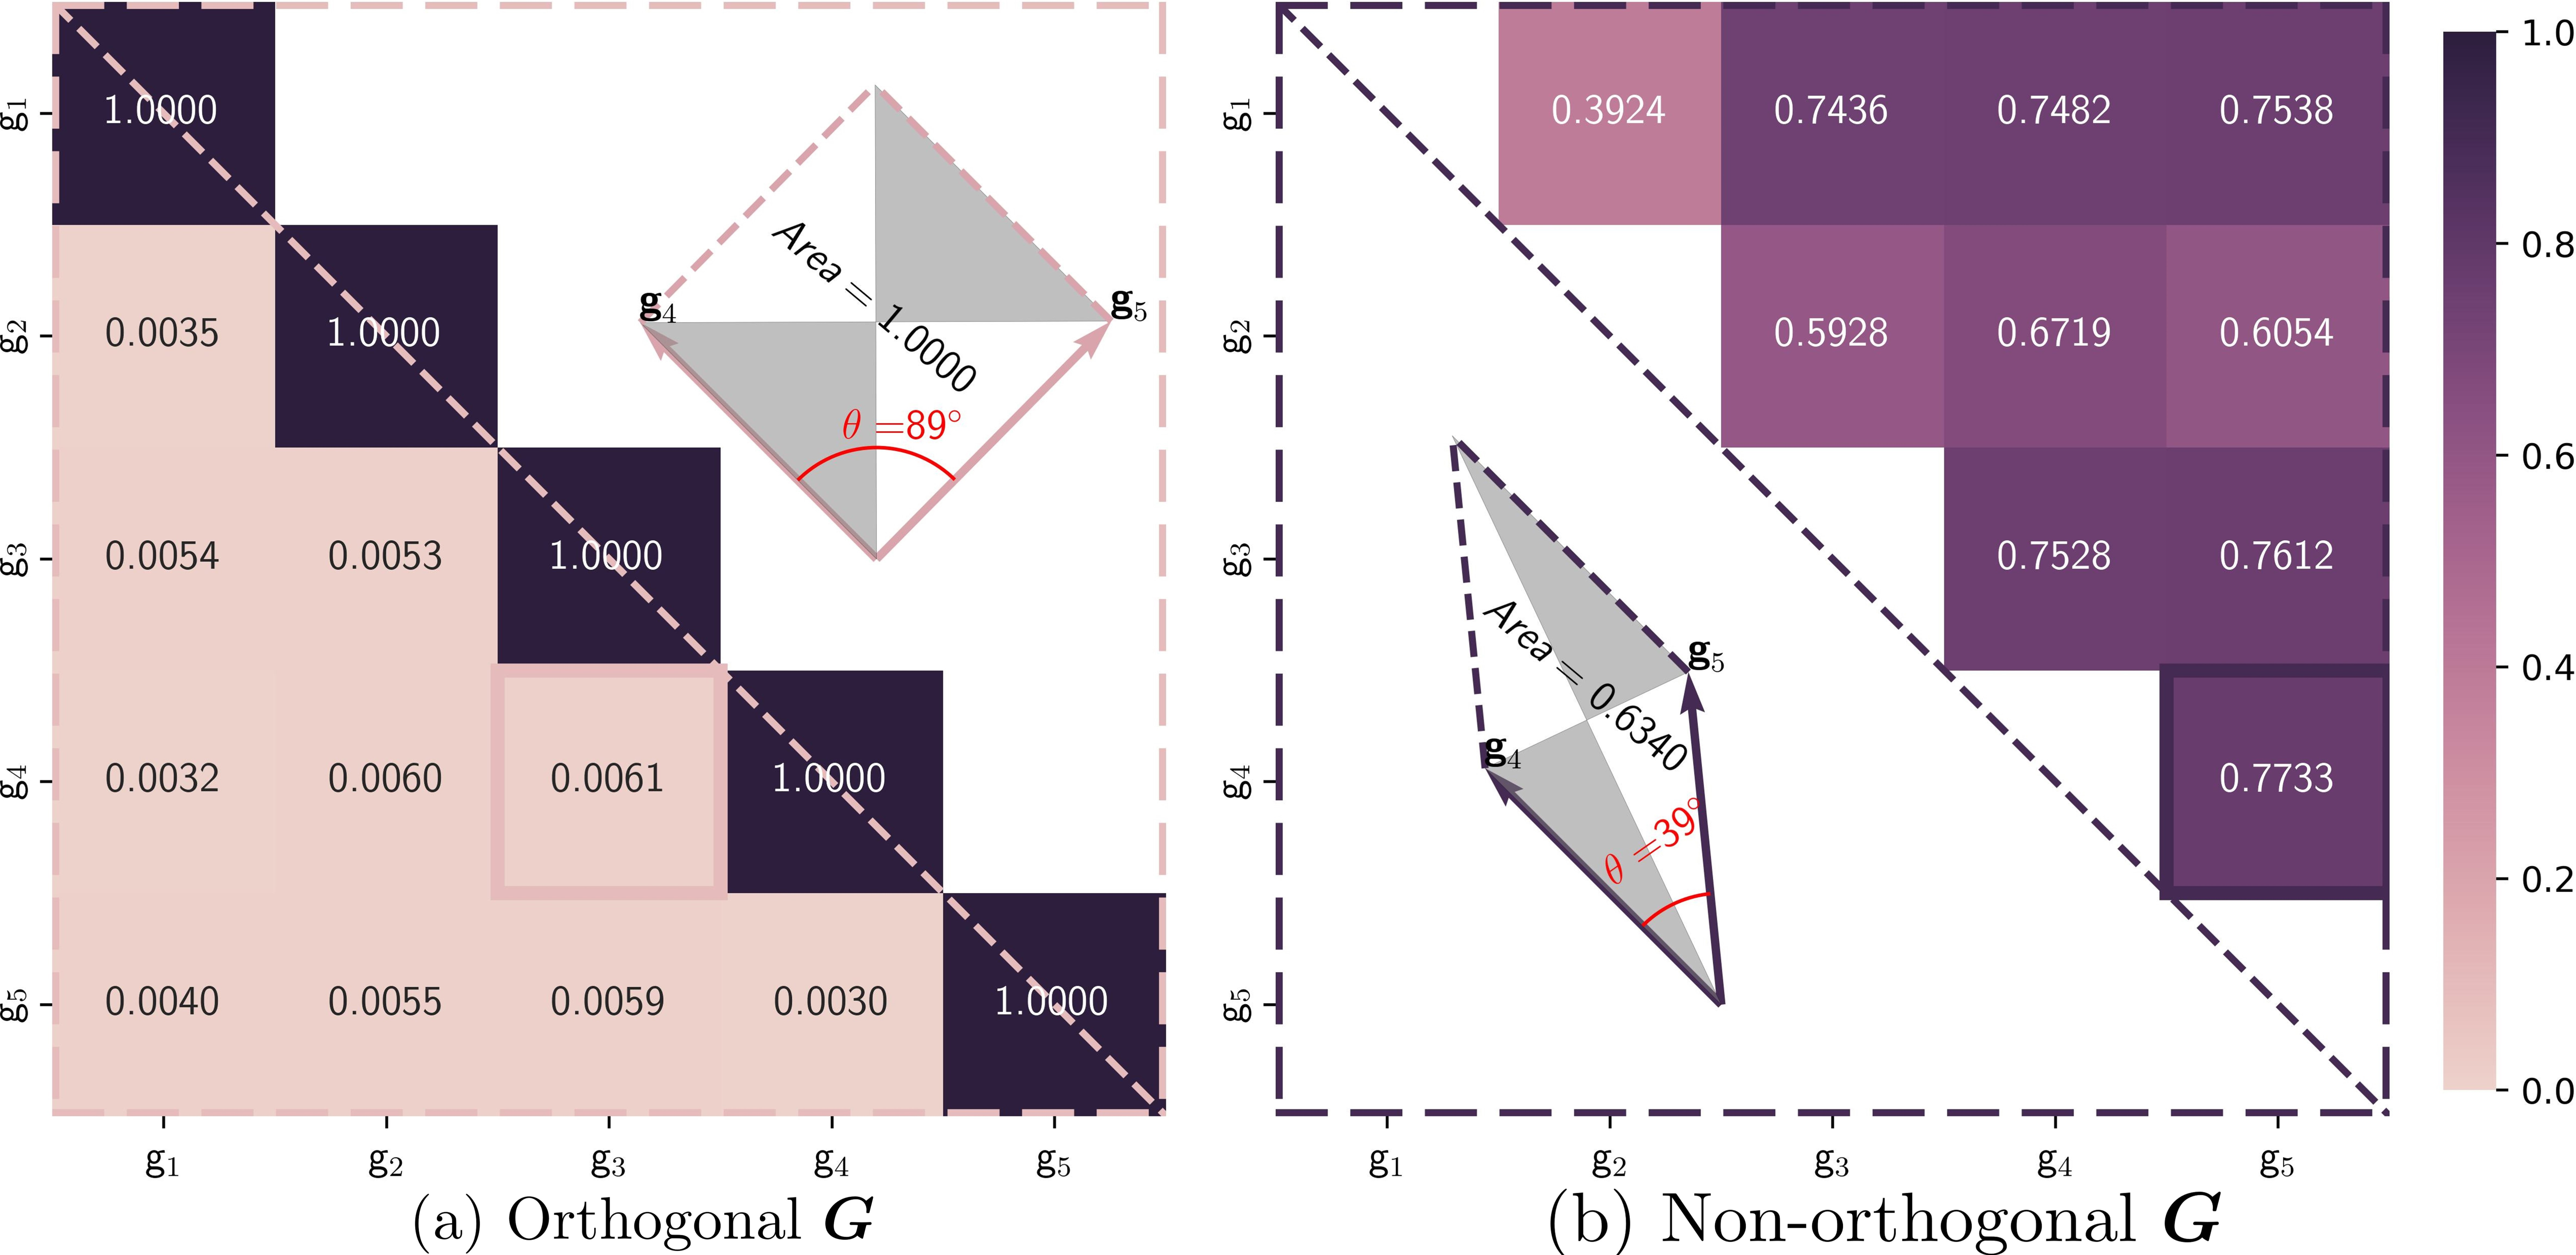
\includegraphics[width=0.75\columnwidth]{Figure/diversity_v2.jpg}
    \caption{The similarity matrix for the global vectors $\boldsymbol{G}$ learned from the CAMELYON16 dataset in two scenarios: (a) $\boldsymbol{G}$ is orthogonal and (b) $\boldsymbol{G}$ is non-orthogonal. To support Lemma~\ref{theorem:geo} and Remark~\ref{remark:div_loss}, we computed the area of the parallelogram corresponding to the two highly correlated global vectors. We omitted the diagonal elements in subpanel figure (b), as $\boldsymbol{L}_{ii}=1, \ \forall i\in [K]$. }
    \label{fig:diversity}
\end{figure}

Lemma~\ref{theorem:geo} immediately implies that a diverse subset is more likely to span larger volumes. This is because as the similarity between two data points (i.e., $\boldsymbol{L}_{ij: i \neq j}$) increases, they will span fewer areas (see Fig. \ref{fig:diversity}(a) and (b)), hence decreasing the probabilities of sets containing both of them (see Eq.(\ref{eqn:dpp})). Accordingly, feature vectors that are more orthogonal to each other span the largest volumes  (see Fig.\ref{fig:diversity}(a)), hence resulting in the most diverse subsets. 

\begin{theorem}\label{theorem:dpp}
Given a set of global vectors $\boldsymbol{G}=[\boldsymbol{g}_1^\top,\cdots,\boldsymbol{g}_K^\top ]$ with $\|\boldsymbol{g}_i\|=C, \forall i\in [K]$,  maximizing the DPP-based diversity (i.e. $\max \operatorname{det}(\boldsymbol{G}\boldsymbol{G}^{\top})$) results in orthogonal global vectors with $\boldsymbol{g}_i \perp \boldsymbol{g}_j, \  \forall i \neq j,i,j \in [K]$.     
\end{theorem}
\begin{proof}
    The determinant $\operatorname{det}(\boldsymbol{L}) = \operatorname{det}(\boldsymbol{G}\boldsymbol{G}^{\top} )$ is upper-bounded according to Hadamard's inequality~\cite{petersen2008matrix}:
    \begin{equation}
    \begin{split}
         &|\operatorname{det}(\boldsymbol{L})|  \overset{(a)}= \operatorname{det}(\boldsymbol{L}) \overset{(b)} \leq \prod_{i=1}^{K} \boldsymbol{L}_{ii}. \\ 
         % & \ \text{s.t.} \ \|\boldsymbol{g}\|_i \leq C, \forall i \in \{1, \cdots, K\},
    \end{split}
    \label{eqn:proof}
    \end{equation}
      \textit{Condition (a)}  is fulfilled because the matrix $\boldsymbol{L}$ is positive semi-definite. The equality of \textit{Condition (b)} is achieved if and only if all non-diagonal entries of $\boldsymbol{G}$ are zeros, meaning rows of the global vectors are orthogonal.
    % The normalization constraint in Eq.(\ref{eqn:proof}) is to prevent the global vectors $\boldsymbol{G}$ from being arbitrarily large, where the upper bound cannot be achieved. 
    The normalization constraint in Eq.(\ref{eqn:proof}) leads the upper bound to be the infimum, since  $\boldsymbol{L}_{ii}=\|\boldsymbol{g}\|_i^2\leq C^2$ and it can be achieved if and only if the equality of \textit{Condition (b)} is satisfied.  
    This completes the proof.
\end{proof}
According to Theorem~\ref{theorem:dpp}, we propose a diversity loss $\mathcal{L}_{div}$ to diversify the proposed global vectors by minimizing the negative logarithm of $\operatorname{det}(\boldsymbol{G}\boldsymbol{G}^{\top})$: 
\begin{equation}
    \mathcal{L}_{div}= -\log\operatorname{det}(\boldsymbol{G}\boldsymbol{G}^{\top}),\quad \text{s.t.} \  \|\boldsymbol{g}_i\|=1=C.
    \label{eqn:div_loss}
\end{equation}
% For arbitrary vector $\boldsymbol{x}$,
% \begin{align}
%     x^\top\boldsymbol{G}\boldsymbol{G}^{\top}x
%     = (x^\top\boldsymbol{G})(\boldsymbol{G}^{\top}x)
%     =(x^\top\boldsymbol{G})^2\geq 0
% \end{align}
% Therefore, $\boldsymbol{G}\boldsymbol{G}^{\top}$ is P.S.D.

\begin{remark}
\label{remark:div_loss}
Theorem~\ref{theorem:dpp} implies that optimal diversity through minimizing our loss is theoretically achievable. This is because enforcing the constraints $\|\boldsymbol{g}_i\|=1$ leads the infimum of $\mathcal{L}_{div}$ to reach zero due to $\log(\boldsymbol{G}\boldsymbol{G}^{\top})_{ii}=\log(\|\boldsymbol{g}_i\|^2)=0$. In contrast, the diversity loss $\mathcal{L}_{div}$ can be arbitrarily small (up to $-\infty$) without the constraint $\|\boldsymbol{g}_i\|=1$, which results in a unstable training.
\end{remark}

% Remark~\ref{remark:div_loss} is also important to stabilize the training because the diversity loss $\mathcal{L}_{div}$ can be arbitrarily small (up to $-\infty$) without the constraint $\|\boldsymbol{g}_i\|=1$ (see the proof of Theorem~\ref{theorem:dpp}).
We also add a small value $\epsilon=1\times 10^{-10}$ to prevent the logarithm of the determinant from being negative infinity (i.e. any two global vectors become collinear). The final diversity loss is given as 
\begin{equation}
    \mathcal{L}_{div}= -\log\operatorname{det}(\boldsymbol{G}\boldsymbol{G}^{\top}+\epsilon\boldsymbol{I}),
\end{equation}
where $\boldsymbol{I}$ denotes the identity matrix. It is noteworthy that the complexity to compute the loss is approximate $ \mathcal{O}(L)$, which is negligible (see Appendix D).

% i) low complexity: for a global vector $\boldsymbol{G}\in \mathbb{R}^{K \times L}$, $\log\operatorname{det}(\boldsymbol{G}\boldsymbol{G}^T)=\sum_{i=1}^K\log(\lambda_i^2)$, where the main overhead is an SVD decomposition of $\boldsymbol{G}$ to get $\lambda_i$, resulting in a complexity of $\mathcal{O}(LK^2)\approx \mathcal{O}(L) $ due to $K$ is often set a small number (e.g., 5) 

\subsection{Objective Function}
The proposed MIL model is trained in an end-to-end fashion by jointly optimizing the weighted combination of cross-entropy (ce) loss that corresponds to the bag-level classification, triplet loss, and the proposed diversity loss:
\begin{equation}
    \mathcal{L}_{final} = \mathcal{L}_{ce} + \lambda_{tri} \mathcal{L}_{tri} + \lambda_{div}\mathcal{L}_{div}, 
\end{equation}
where $\lambda_{tri}$ and $\lambda_{tri}$ are balance parameters.

% \begin{figure*}[!t]
% \centering
% 
\includegraphics[width=1.0\textwidth]{Figure/params.jpg} % Reduce the figure size to slightly narrower than the column.
% \caption{Ablation studies on (a) number of non-tokenized global vectors on both CAMELYON16 and TCGA-NSCLC datasets, (b) and (c) balance parameter $\lambda_{tri}$ and $\lambda_{div}$ on CAMELYON16 dataset, respectively. (d) Comparison in the number of positive instances per bag.}
% \label{fig:Ablation}
% \end{figure*}


\section{Experiments and Results}
To validate the effectiveness of the proposed DGR-MIL, we conduct experiments on the CAMELYON16 dataset~\cite{bejnordi2017diagnostic} and TCGA-lung cancer dataset (TCGA-NSCLC).

\noindent\textbf{Dataset and Evaluation Metrics.} The two datasets are followed the experimental data partition setting in~\cite{zhang2022dtfd}. For the CAMELYON16, the training set is further divided into training and validation sets with a 9:1 ratio. We report the mean of accuracy, F1 score, and AUC with their corresponding $95\%$ interval on the testing dataset after running five experiments. For the TCGA lung cancer dataset, we perform 4-fold cross-validation experiments, where the dataset is partitioned into training, validation, and testing sets with a patient ratio of 65:10:25.  We report the mean and standard variation of accuracy, F1 score, and AUC on the testing dataset from 4-fold cross-validation.

\noindent\textbf{Experiment Setup.}
Three sets of instance features were extracted using different strategies to evaluate the proposed method's adaptability across various feature embeddings. The first set provided by DTFD-MIL~\cite{zhang2022dtfd}, employing OTSU's method for patch extraction from WSIs and ResNet-50 for feature extraction, resulting in 1024-dimensional vectors per patch. For thorough validation, two additional sets of features were generated by segmenting each WSI into non-overlapping 224x224 patches using threshold filtering, resulting in 3.4 and 10.3 million patches from CAMELYON16 and TCGA lung cancer datasets~\cite{li2021dual,qiu2023sc,lin2023interventional,PDL}, respectively. These patches were processed using ResNet-18 and Vision Transformer, pre-trained on ImageNet, to produce 512 and 768-dimensional feature vectors.



\noindent\textbf{Baseline MIL Models.}
 We compare the proposed model to eight state-of-the-art MIL methods. These models can be roughly divided into two categories: i) AB-MIL~\cite{ilse2018attention} and its variants, including CLAM-SB~\cite{clam-sb}, DS-MIL~\cite{li2021dual}, and DTFD-MIL~\cite{zhang2022dtfd}; ii) the transformer-based methods including Trans-MIL~\cite{shao2021transmil} and ILRA-MIL~\cite{lowrankmil}. iii) clustering/prototype-based MIL including PMIL~\cite{pmil}.
% Following the experiment setting~\cite{zhang2022dtfd},

\begin{table*}[t]		
\caption{Main results on the CAMELYON16 dataset and TCGA-NSCLC dataset by using features extracted by different means. Our method statistically outperforms all other competitors (refer to the statistic test in Appendix E)}
\label{tab:experiment_two_benchmark}
		\centering
		\resizebox{1.0\textwidth}{!}{
			\begin{tabular}{lccc|ccc}
				\toprule
                     & \multicolumn{3}{c}{CAMELYON16} & \multicolumn{3}{c}{TCGA-NSCLC} \\
                      \cmidrule(r){2-4} \cmidrule(r){5-7}
				  & Accuracy & F1 &  AUC & Accuracy & F1 &  AUC  \\
				\midrule
				& \multicolumn{6}{c}{\cellcolor{blue!20}\bf ResNet-50 ImageNet Pretrained } \\
                     Classic AB-MIL (\textit{ICML'18})   & $0.845_{(0.839,0.851)}$& $0.780_{(0.769,0.791)}$ & $0.854_{(0.848,0.860)}$ &$0.869_{0.032}$ & $0.866_{0.021}$ & $0.941_{0.028}$\\ %
   
                      DS-MIL (\textit{CVPR'21})  &$0.856_{(0.843,0.869)}$  &$0.815_{(0.797,0.832)}$  &$0.899_{(0.890,0.908)}$  &$0.888_{0.013}$ & $0.876_{0.011}$ &$0.939_{0.019}$\\ %
                    CLAM-SB (\textit{Nature Bio. Eng.'21}) & $0.837_{(0.809,0.865)}$ & $0.775_{(0.755,0.795)}$ & $0.871_{(0.856,0.885)}$ & $0.875_{0.041}$ & $0.864_{0.043}$ & $0.944_{0.023}$\\ %
                    CLAM-MB (\textit{Nature Bio. Eng.'21})  &$0.823_{(0.795,0.850)}$ & $0.774_{(0.752,0.795)}$& $0.878_{(0.861,0.894)} $& $0.878_{0.043} $& $0.874_{0.028}$ & $0.949_{0.019}$\\ %
                    PMIL (\textit{MedIA'23})  &$0.831_{(0.799,0.863)}$& $0.816_{(0.779,0.853)}$ & $0.845_{(0.813,0.876)} $ & $0.873_{0.010}$ &$0.875_{0.011}$ &$0.933_{0.007}$ 
                    \\% 
                    Trans-MIL (\textit{NeurIPS'21}) & $0.858_{(0.848,0.868)}$  & $0.797_{(0.776,0.818)}$  & $0.906_{(0.875,0.937)}$ & $0.883_{0.022}$  & $0.876_{0.021}$  & $0.949_{0.013}$ \\ %
                    
                    DTFD-MIL (MaxS) (\textit{CVPR'22})  &$0.864_{(0.848,0.880)} $& $0.814_{(0.802,0.826)}$& $0.907_{(0.894,0.919)} $&$ 0.868_{0.040 }$& $0.863_{0.029}$& $0.919_{0.037}$
                    \\ %
                    DTFD-MIL (MaxMinS) (\textit{CVPR'22})  &$0.899_{(0.887,0.912)}$ & $0.865_{(0.848,0.882)}$ & $0.941_{(0.936,0.944)}$ & $0.894_{0.033}$ & $0.891_{0.027}$ & $0.961_{0.021}$ \\ %
                    DTFD-MIL (AFS) (\textit{CVPR'22})  & $0.908_{(0.892,0.925)}$ & $0.882_{(0.861,0.903)}$ & $0.946_{(0.941,0.951)}$ & $0.891_{0.033}$ & $0.883_{0.025}$ & $0.951_{0.022}$
                    \\%
                    ILRA-MIL (\textit{ICLR'23}) 
                    &$0.848_{(0.844,0.853)}$& $0.826_{(0.823,0.829)}$ & $0.868_{(0.852,0.883)} $  & $0.895_{0.017}$ &$0.896_{0.017}$ &$0.946_{0.014}$  
                      \\                 
                     \rowcolor{blue!8} 
                     % \rowcolor{yellow!18} 
                     \textbf{Our}  
%                      &$0.917
% _{(0.902
% ,0.931)}$& $0.913_{(0.898,0.928)}$ & $0.957_{(0.951,0.963)} $ & $0.908_{0.015}$ &$0.911_{0.018}$ &$0.963_{0.008}$  
&$\mathbf{0.917}_{(0.902, 0.931)}$& $\mathbf{0.913}_{(0.898, 0.928)}$ & $\mathbf{0.957}_{(0.951, 0.963)}$ & $\mathbf{0.908}_{0.015}$&$\mathbf{0.911}_{0.018}$&$\mathbf{0.963}_{0.008}$

\\ 
                     
                 \hline
                    & \multicolumn{6}{c}{\cellcolor{blue!20}\bf ResNet-18 ImageNet Pretrained} \\
                    Classic AB-MIL (\textit{ICML'18})  & $0.805_{(0.772,0.837)}$& $0.786_{(0.757,0.815)}$ & $0.843_{(0.827,0.858)}$ &$0.874_{0.005}$ & $0.873_{0.006}$ & $0.937_{0.001}$\\ %
   
                    DS-MIL (\textit{CVPR'21})  &$0.791_{(0.739,0.843)}$  &$0.776_{(0.712,0.840)}$  &$0.814_{(0.754,0.875)}$  &$0.831_{0.012}$ & $0.838_{0.008}$ &$0.896_{0.009}$\\ %
                    CLAM-SB (\textit{Nature Bio. Eng.'21})  & $0.792_{(0.769,0.815)}$ & $0.766_{(0.746,0.786)}$ & $0.811_{(0.777,0.845)}$ & $0.869_{0.010}$ & $0.869_{0.010}$ & $0.931_{0.006}$\\ %
                    CLAM-MB (\textit{Nature Bio. Eng.'21}) &$0.786_{(0.754,0.818)}$ & $0.770_{(0.746,0.795)}$& $0.825_{(0.808,0.843)} $& $0.880_{0.016} $& $0.880_{0.016}$ & $0.944_{0.012}$\\ %
                    PMIL (\textit{MedIA'23})  &$0.800_{(0.775,0.825)}$& $0.784_{(0.765,0.804)}$ & $0.829_{(0.807,0.851)} $ 
                     & $0.856_{0.006}$ &$0.862_{0.003}$ &$0.933_{0.010}$\\%     
                    Trans-MIL (\textit{NeurIPS'21}) & $0.839_{(0.822,0.856)}$  & $0.827_{(0.805,0.848)}$  & $0.854_{(0.823,0.886)}$ & $0.877_{0.009}$  & $0.879_{0.008}$  & $0.938_{0.014}$ \\ %
                    
                    DTFD-MIL (MaxS) (\textit{CVPR'22})  &$0.856_{(0.824,0.887)} $& $0.792_{(0.742,0.842)}$& $0.878_{(0.862,0.893)} $&$ 0.830_{0.014 }$& $0.821_{0.020}$& $0.893_{0.015}$
                    \\ %
                    DTFD-MIL (MaxMinS) (\textit{CVPR'22})  &$0.833_{(0.807,0.858)}$ & $0.768_{(0.747,0.788)}$ & $0.878_{(0.872,0.883)}$ & $0.853_{0.012}$ & $0.850_{0.021}$ & $0.925_{0.013}$ \\ %
                    DTFD-MIL (AFS) (\textit{CVPR'22})  & $0.817_{(0.791,0.843)}$ & $0.734_{(0.687,0.781)}$ & $0.868_{(0.841,0.896)}$ & $0.870_{0.007}$ & $0.864_{0.012}$ & $0.935_{0.010}$
                    \\%
                    ILRA-MIL (\textit{ICLR'23})  &$0.831_{(0.768,0.895)}$& $0.819_{(0.768,0.871)}$ & $0.852_{(0.811,0.893)} $ & $0.878_{0.002}$ &$0.879_{0.001}$ &$0.937_{0.004}$  

\\                  
                     \rowcolor{blue!8}
                     % \rowcolor{yellow!18} 
                     \textbf{Our} 
&$\mathbf{0.873}_{(0.862, 0.884)}$& $\mathbf{0.862}_{(0.852, 0.871)}$ & $\mathbf{0.898}_{(0.886, 0.909)}$ & $\mathbf{0.891}_{0.029}$&$\mathbf{0.890}_{0.021}$&$\mathbf{0.955}_{0.023}$

\\ 
                    
                \hline
                 & \multicolumn{6}{c}{\cellcolor{blue!20}\bf Vision Transformer ImageNet Pretrained } \\
                     Classic AB-MIL (\textit{ICML'18})   & $0.851_{(0.837,0.865)}$& $0.835_{(0.810,0.860)}$ & $0.873_{(0.840,0.906)}$ &$0.904_{0.011}$ & $0.904_{0.010}$ & $0.953_{0.013}$\\ %
   
                    DS-MIL (\textit{CVPR'21})  &$0.810_{(0.741,0.879)}$  &$0.806_{(0.742,0.869)}$  &$0.871_{(0.836,0.906)}$  &$0.875_{0.020}$ & $0.879_{0.016}$ &$0.933_{0.016}$\\ %
                    CLAM-SB (\textit{Nature Bio. Eng.'21}) & $0.839_{(0.831,0.847)}$ & $0.816_{(0.799,0.834)}$ & $0.864_{(0.841,0.887)}$ & $0.907_{0.008}$ & $0.907_{0.001}$ & $0.954_{0.014}$\\ %
                    CLAM-MB (\textit{Nature Bio. Eng.'21}) &$0.826_{(0.806,0.846)}$ & $0.804_{(0.795,0.813)}$& $0.851_{(0.825,0.878)} $& $0.911_{0.007} $& $0.911_{0.007}$ & $0.959_{0.008}$\\ %
                    PMIL (\textit{MedIA'23})  &$0.843_{(0.831,0.856)}$& $0.826_{(0.814,0.838)}$ & $0.843_{(0.820,0.867)} $ 
                     & $0.882_{0.009}$ &$0.884_{0.006}$ &$0.940_{0.006}$
                     \\
                    Trans-MIL (\textit{NeurIPS'21}) & $0.862_{(0.841,0.883)}$  & $0.846_{(0.823,0.869)}$  & $0.860_{(0.848,0.873)}$ & $0.909_{0.009}$  & $0.909_{0.009}$  & $0.953_{0.006}$ \\ %
                    
                    DTFD-MIL (MaxS) (\textit{CVPR'22}) & $0.846_{(0.832,0.860)}$& $0.767_{(0.746,0.787)}$ & $0.859_{(0.842,0.876)}$ &$0.904_{0.011}$ & $0.904_{0.010}$ & $0.953_{0.013}$
                    \\
                    DTFD-MIL (MaxMinS) (\textit{CVPR'22})  &$0.839_{(0.826,0.851)}$ & $0.752_{(0.742,0.763)}$ & $0.862_{(0.836,0.888)}$ & $0.895_{0.013}$ & $0.892_{0.016}$ & $0.952_{0.011}$ \\ %
                    DTFD-MIL (AFS) (\textit{CVPR'22})  & $0.831_{(0.818,0.844)}$ & $0.759_{(0.737,0.781)}$ & $0.880_{(0.864,0.897)}$ & $0.901_{0.005}$ & $0.900_{0.008}$ & $0.959_{0.012}$
                    \\%
                    ILRA-MIL (\textit{ICLR'23})  &$0.850
_{(0.825
,0.875)}$& $0.838
_{(0.812
,0.865
)}$ & $0.864
_{(0.843
,0.885
)} $ & $0.902_{0.007}$ &$0.904_{0.007}$ &$0.954_{0.006}$  
        
                     
                     \\
                     % 
                     % \rowcolor{blue!8} 
                     % \rowcolor{yellow!18} 
                     \rowcolor{blue!8}
                     \textbf{Our}  
                     % & $0.893_{(0.889,0.897)}$ & $0.882_{(0.877,0.886)} $ & $0.891_{(0.884,0.899)}$&$0.926_{0.008}$ &$0.925_{0.008}$ &$0.969_{0.004}$ 
                    & $\mathbf{0.893}_{(0.889,0.897)}$ & $\mathbf{0.882}_{(0.877,0.886)}$ & $\mathbf{0.891}_{(0.884,0.899)}$ & $\mathbf{0.926}_{0.008}$ & $\mathbf{0.925}_{0.008}$ & $\mathbf{0.969}_{0.004}$

                     
                     \\ 
                     
				\bottomrule
 			\end{tabular}}

   \vspace{-0.5cm}
\end{table*}
\noindent\textbf{Implementation Details.}  All the models are trained using the parameter settings provided by~\cite{shao2021transmil,zhang2022dtfd,li2021dual,clam-sb,lowrankmil}. (See Appendix B, including our method). 


\noindent\textbf{Additional Experiments.} We also include the experiments on using CTransPath \cite{wang2022transformer} as feature extractor for CAMELYON16 dataset. Additionally, to validate the generalizability of our method on broader applications other than WSI, we conduct the experiment on MIL benchmark \cite{dietterich1997solving,andrews2002support}. Our method demonstrates the obvious superiority over other methods in both experiments. Please refer to Appendix F.


% \begin{figure*}[!t]
% \centering
% 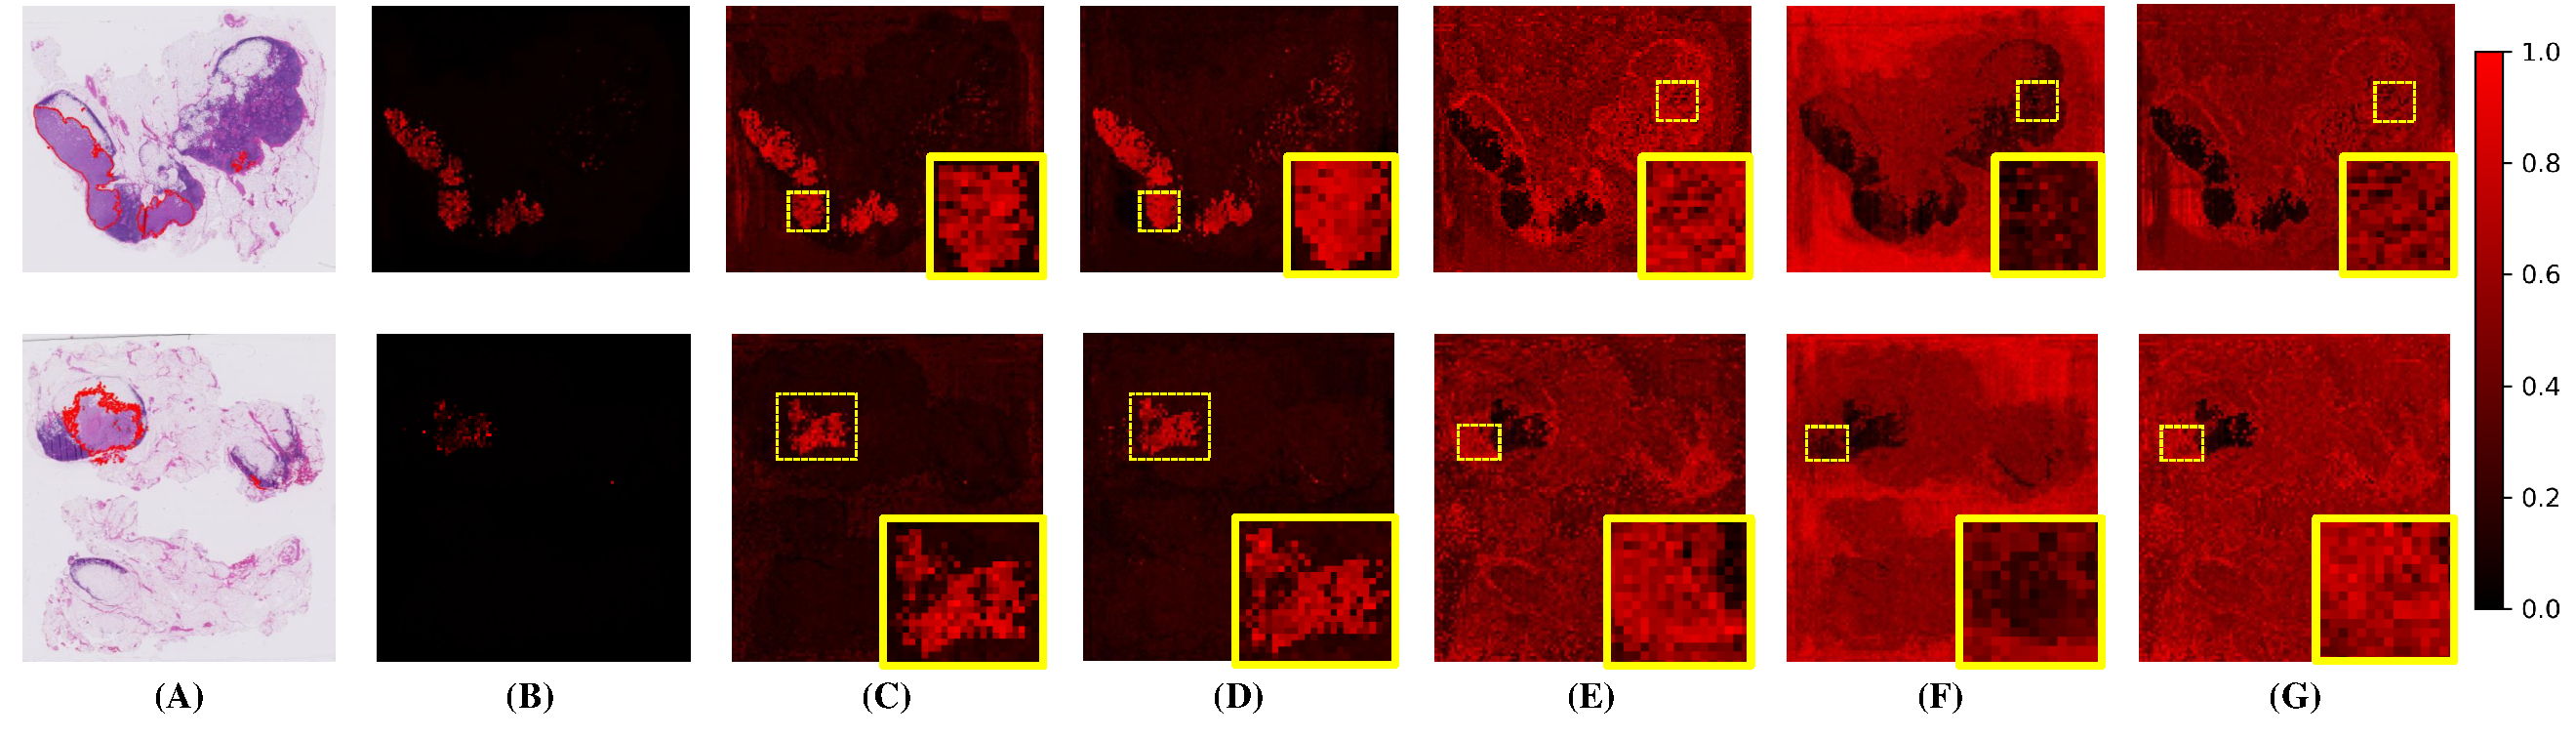
\includegraphics[width=0.95\textwidth]{Figure/visulization.jpg} % Reduce the figure size to slightly narrower than the column.
% \caption{Visualization of the attention map: (a) raw WSI with the ground-truth annotation, (b) the attention map computes using the tokenized global vectors, and (c-g) the attention map computes using the other ($K-1$) global vectors with $K=6$ in our experiment. }
% \label{fig:visulization}
% \end{figure*}

\subsection{Experimental Results}
The proposed method outperforms the other state-of-the-art MIL aggregation models by a large margin in both the CAMELYON16 and TCGA-NSCLC datasets using features extracted by three different means (see Table~\ref{tab:experiment_two_benchmark}). We also show the statistical superiority of our method in Appendix E. Specifically, the proposed model outperforms the second-best models in terms of accuracy (1.7\%; 1.3\%), F1 score (3.1\%; 1.5\%), and AUC (1.1\%; 1.7\%) when using features extracted from ResNet-50 in CAMELYON16 and TCGA-NSCLC, respectively. 
A similar performance gain is observed on features extracted from ResNet-18 including accuracy (3.4\%; 1.1\%), F1 score (3.5\%; 1.0\%), and AUC (4.4\%; 1.1\%). We also observe an improvement in accuracy (3.4\%; 1.1\%), F1 score (3.5\%; 1.0\%), and AUC (4.4\%; 1.1\%) when using features extracted from the vision transformer. In general, the proposed model shows a greater performance improvement in the CAMELYON16 dataset compared to the TCGA-NSCLC dataset. This might be attributed to the fact that CAMELYON16 consists of more diverse instances than TCGA-NSCLC. 

We also observe the performance of the three sets of feature embeddings varied: the ViT feature embeddings outperform the ResNet-18 features but show inferior performance compared to the ResNet-50 features. This is mainly attributed to the fact that a greater number of positive instances is extracted by the ResNet-50 (provided by DTFD-MIL) as shown in Fig. \ref{fig:Ablation}(d). In contrast, a smaller portion of positive instances in the extracted patches may accompany a drop in performances~\cite{plp2}. This phenomenon benefits the pseudo-bag partitions in DTFD-MIL, as more positive instances within a bag are prone to result in less noisy pseudo-bag labels. This accounts for the drop in DTFD-MIL performance when applied to feature embeddings that contain a lower proportion of positive instances.

\subsection{Ablation Studies}
We conduct ablation studies on model design variants in the CAMELYON16 dataset with features extracted by a ResNet-50, unless specified otherwise. 
\begin{figure*}[!t]
\centering

\includegraphics[width=1.0\textwidth]{Figure/params.jpg} % Reduce the figure size to slightly narrower than the column.
\caption{Ablation studies on (a) number of non-tokenized global vectors on both CAMELYON16 and TCGA-NSCLC datasets, (b) and (c) balance parameter $\lambda_{tri}$ and $\lambda_{div}$ on CAMELYON16 dataset, respectively. (d) Comparison in the number of positive instances per bag.}
\label{fig:Ablation}
\end{figure*}

% The Figure~\ref{fig:Ablation}, we present how 

% Please add the following required packages to your document preamble:
% \usepackage{graphicx}

% Please add the following required packages to your document preamble:
% \usepackage{graphicx}


\begin{table}[!t]
\vspace{-0.2cm}
    \centering
     % \caption{Comparison of different Datasets (\textbf{Left}): XXX (\textbf{Right}): Glas and MoNuSeg. }
    \begin{minipage}{0.45\columnwidth}
        
        \centering
\caption{The ablation studies on different modules. $\mathcal{P}$: Positive instance alignment module. $\mathcal{D}$: Diversity loss.}
% where $\mathcal{P}$ and $\mathcal{D}$ denote the positive instance alignment module and the DPP-driven diversity learning, respectively.}
\label{tab:aba_table1}
\resizebox{1\textwidth}{!}{%
\begin{tabular}{ll|ccc|ccc}
\toprule %
 $\mathcal{P}$ & $\mathcal{D}$ & \multicolumn{3}{c}{CAMELYON16} & \multicolumn{3}{c}{TCGA-NSCLC} \\
                      \cmidrule(r){3-5} \cmidrule(r){6-8}
				&  & Accuracy & F1 &  AUC & Accuracy & F1 & AUC  \\
				\midrule
\ding{55} & \ding{55} & \textcolor{gray}{0.895}  & \textcolor{gray}{0.887} & \textcolor{gray}{0.922}  & \textcolor{gray}{0.872} & \textcolor{gray}{0.875} & \textcolor{gray}{0.928}\\ 
\ding{55} &\ding{51}  & 0.906 & 0.900 & 0.938 & 0.896 & 0.896 & 0.952 \\
  \ding{51}& \ding{55} & 0.917 & 0.910 & 0.944 & 0.900 & 0.904 & 0.956 \\
% \ding{55} & \ding{51} & \ding{51} & 0.907 & 0.900 & 0.935 \\ 
 \ding{51}& \ding{51} & 0.917 & 0.913 & 0.957 & 0.908 & 0.911 & 0.963 \\

\bottomrule
\end{tabular}%
}
    \end{minipage}%
    \hfill
    \begin{minipage}{0.5\columnwidth}
    \centering
    \caption{ The ablation studies on tokenized global representation.}
\label{tab:token}
\resizebox{1\textwidth}{!}{%
\begin{tabular}{c|ccc|ccc}
\toprule %
 $\boldsymbol{g}_{\operatorname{token}}$ & \multicolumn{3}{c}{CAMELYON16} & \multicolumn{3}{c}{TCGA-NSCLC} \\
                      \cmidrule(r){2-4} \cmidrule(r){5-7}
				  & Accuracy & F1 &  AUC & Accuracy & F1 &  AUC  \\
				\midrule


 \ding{55} & 0.907 & 0.900 & 0.935 & 0.903 & 0.905 & 0.957 \\
 \ding{51} & 0.917 & 0.913 & 0.957 & 0.908 & 0.911 & 0.963 \\ 
 \bottomrule
\end{tabular}%
}
\vspace{-0.2cm}
    \end{minipage}
% \vspace{-0.3cm}
\end{table}


% \begin{table}[!t]
% \centering
% \caption{The ablation studies on modules in our framework where $\mathcal{P}$ and $\mathcal{D}$ denote the positive instance alignment module and the DPP-driven diversity learning, respectively.}
% \label{tab:aba_table1}
% \resizebox{0.4\textwidth}{!}{%
% \begin{tabular}{ll|ccc|ccc}
% \toprule %
%  $\mathcal{P}$ & $\mathcal{D}$ & \multicolumn{3}{c}{CAMELYON16} & \multicolumn{3}{c}{TCGA-NSCLC} \\
%                       \cmidrule(r){3-5} \cmidrule(r){6-8}
% 				&  & Accuracy & F1 &  AUC & Accuracy & F1 & AUC  \\
% 				\midrule
% \ding{55} & \ding{55} & \textcolor{gray}{0.895}  & \textcolor{gray}{0.887} & \textcolor{gray}{0.922}  & \textcolor{gray}{0.872} & \textcolor{gray}{0.875} & \textcolor{gray}{0.928}\\ 
% \ding{55} &\ding{51}  & 0.906 & 0.900 & 0.938 & 0.896 & 0.896 & 0.952 \\
%   \ding{51}& \ding{55} & 0.917 & 0.910 & 0.944 & 0.900 & 0.904 & 0.956 \\
% % \ding{55} & \ding{51} & \ding{51} & 0.907 & 0.900 & 0.935 \\ 
%  \ding{51}& \ding{51} & 0.917 & 0.913 & 0.957 & 0.908 & 0.911 & 0.963 \\

% \bottomrule
% \end{tabular}%
% }
% \vspace{-0.2cm}
% \end{table}


% \begin{table}[!t]
% \centering
% \label{tab:token}
% \resizebox{0.5\textwidth}{!}{%
% \begin{tabular}{l|ccc|ccc}
% \toprule %
%  $\boldsymbol{g}_{\operatorname{token}}$ & \multicolumn{3}{c}{CAMELYON16} & \multicolumn{3}{c}{TCGA-NSCLC} \\
%                       \cmidrule(r){2-4} \cmidrule(r){5-7}
% 				  & Accuracy & F1 &  AUC & Accuracy & F1 &  AUC  \\
% 				\midrule
%  \ding{55} & 0.907 & 0.900 & 0.935 & 0.908 & 0.911 & 0.963\\
%  \ding{51} & 0.917 & 0.913 & 0.957 & 0.908 & 0.911 & 0.963 \\ 
%  \bottomrule
% \end{tabular}%
% }
% \vspace{-0.2cm}
% \end{table}





\noindent\textbf{Effectiveness of the Proposed Global Representation.} 
We ablate different components of the proposed model, i.e., the positive instance alignment module and the diversity loss. While the model without these two components serves as the baseline in Table~\ref{tab:aba_table1}.
We first observe that incorporating the proposed global vectors described in Section~\ref{sec:grmp}
(without employing any of the learning strategies in Section~\ref{sec:GRCL}) yielded an AUC of 0.922 and 0.928. This AUC exceeds that of most existing MIL models, except for DTFD-MIL (MaxMinS \& AFS) (see Table~\ref{tab:experiment_two_benchmark} and~\ref{tab:aba_table1}). 
Subsequently, by including the proposed positive instance alignment module, we observe a performance gain of (2.2\%, 2.8\%) in accuracy, (2.3\%, 2.9\%) in F1 score, and (2.2\%, 2.8\%) in AUC. Up to now, we outperform the DTFD-MIL in terms of accuracy and F1 score (see Table~\ref{tab:experiment_two_benchmark} and~\ref{tab:aba_table1}), and achieve a similar AUC (AUC = 0.944,0.956) compare to the DTFD-MIL(AFS) (AUC = 0.946,0.951). Further incorporating the proposed diversity loss into the objective function yields a performance gain of (1.3\%,0.7\%) in AUC, which outperforms DTFD-MIL (AFS) by (1.1\%,1.2\%). 


\begin{figure*}[!t]
\centering
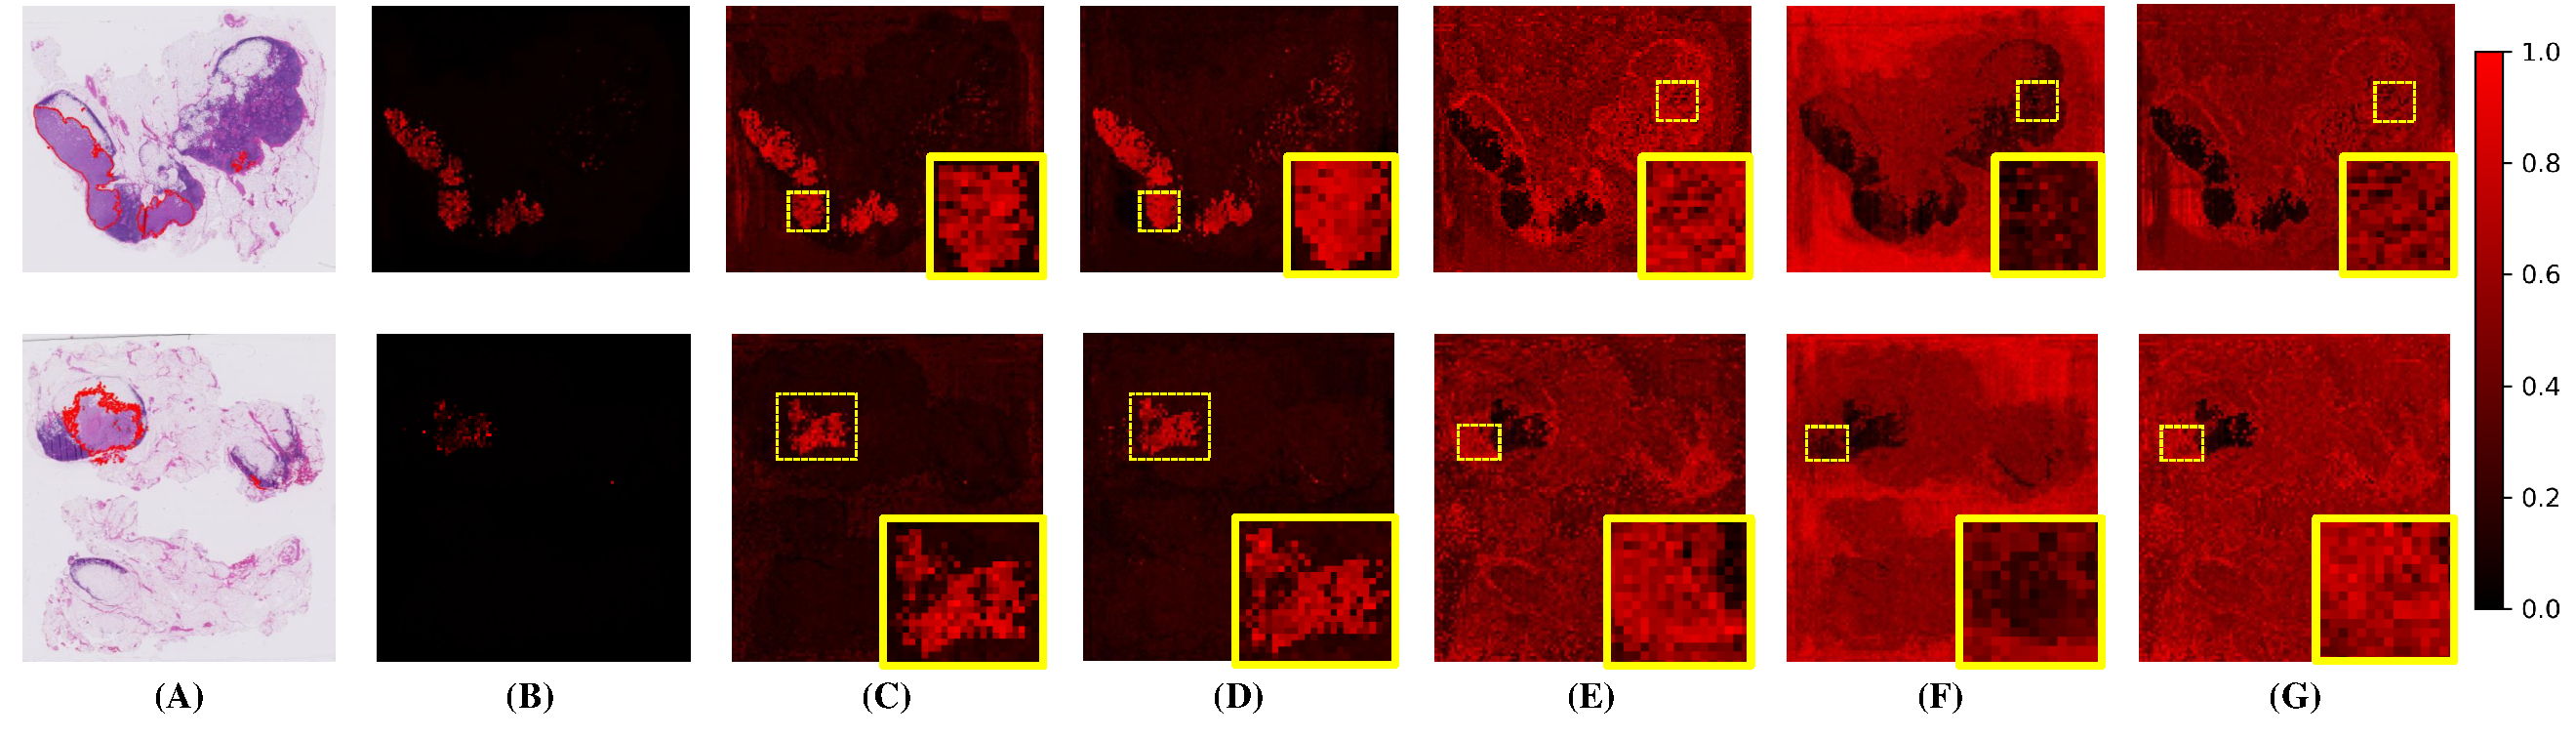
\includegraphics[width=0.95\textwidth]{Figure/visulization.jpg} % Reduce the figure size to slightly narrower than the column.
\caption{Visualization of the attention map: (a) raw WSI with the ground-truth annotation, (b) the attention map computes using the tokenized global vectors, and (c-g) the attention map computes using the other ($K-1$) global vectors with $K=6$ in our experiment. }
\label{fig:visulization}
\vspace{-0.3cm}
\end{figure*}

\noindent\textbf{Effectiveness of the Tokenized Global Representation.} As shown in Table \ref{tab:token}, including the tokenized global vector $\boldsymbol{g}_{\operatorname{token}}$ yields a remarkable performance gain by improving accuracy by (1.0\%, 0.5\%), F1 score by (1.3\%, 0.6\%), and AUC by (2.2\%, 0.6\%). As consistent with the pathological findings that instances are diverse, we observe that different global vectors indeed corresponded to different instance representations, which can be depicted by the attention map produced by different global vectors in Fig. \ref{fig:visulization}. 
However, we also observe that the learned global vectors still include non-tumor related representation, particularly around tumor boundaries, as positive instances around tumor boundaries have a similar appearance to surrounding negative instances (see Fig. \ref{fig:visulization}.(c) and (d)). As a result, incorporating tokenized global vectors can mitigate this problem by capturing the most discriminative positive (tumor) regions (see Fig. \ref{fig:visulization}.(b)). 


\noindent\textbf{Number of Global Vectors.} We find that the optimal number of global vectors $K$ in different data sets may vary due to dataset intrinsic properties. 
Specifically, the optimal $K$ for the CAMELYON16 and TCGA-NSCLC dataset are $K=5$ and $K=3$, respectively (Fig. \ref{fig:Ablation}.(a)). 
We observe that an overly large $K$ is likely to decrease performance as it will harden the learning task (see Fig. \ref{fig:Ablation}.(a)). 

\noindent\textbf{Loss Balance Hyperparameters.} 
By conducting a grid search, we find that the optimal setting of the balance parameters is $\lambda_{tri} = 0.1$ and $\lambda_{div} = 0.1$ (see Fig. \ref{fig:Ablation}.(b) and (c)). An overly small $\mathcal{L}_{tri}$ and $\mathcal{L}_{div}$  (e.g., $0.01$) is likely to enforce inadequate constraints on the learned global representation by deviating it from learning meaningful information of instance of interest. While larger balance parameters (e.g., $\{0.5, 1.0\}$) distract the model from the main classification task, leading to a drop in classification performance. 


\begin{comment}

\end{comment}
\section{Conclusion}
Inspired by the pathological fact that instances are diverse, we propose a novel MIL model from the perspective of modeling diversity in instances through the cross-attention between instances and a set of learnable and diverse global vectors. To learn the global vectors, we propose a positive instance alignment mechanism and the DPP-driven diversity loss. Extensive experiments demonstrate that the proposed MIL model competed favorably against other existing MIL models. Importantly, our work provides an explicit way to account for the diversity in WSI. This pathology-driven approach is beneficial in capturing heterogeneity among the patient population. We also narrowed the performance gap between the diversity-drive MIL method and mainstream MIL.

% \begin{table}[]
%     \centering
%     \begin{tabular}{|c|c|c|c|}
%     \hline
%         Number of Global Lesions & Acc & F1 & AUC  \\
%         \hline
%         1 &0.898 &0.891 & 0.935
% \\
%         \hline
%         3 &0.925& 0.919& 0.947
% \\
%         \hline
%         5 & & & \\
%         \hline
%         7 &0.892&0.884& 0.932
% \\
%         \hline
%         9 &0.882
%  &0.895
%  &0.933
%  \\
%     \hline
%     \end{tabular}
%     \caption{Ablation study on the number of global lesions.}
%     \label{tab:my_label}
% \end{table}

% \begin{table}[]
%     \centering
%     \begin{tabular}{|c|ccc|c|c|c|c|}
%     \hline
%         Index & $\mathcal{P}$ & $\mathcal{D}$ & $\mathcal{T}$ & Acc & F1 & AUC  \\
%         \hline
%         1 & $\surd$ & &  & & & \\
%         % \hline
%         2 &  & $\surd$ &  & & & \\
%         3 &  &  &  $\surd$ & & & \\
%         4 & $\surd$ & $\surd$ &  & & & \\
%         5 & $\surd$ & & $\surd$   & & & \\
%         6 &  & $\surd$ & $\surd$ & & & \\
%         7 & $\surd$ & $\surd$ &  $\surd$ &0.940 &0.937 &0.970 \\
%     \hline
%     \end{tabular}
%     \caption{Ablation study on losses.}
%     \label{tab:my_label}
% \end{table}

% \begin{table}[]
%     \centering
%     \begin{tabular}{|ccc|c|c|c|}
%     \hline
%          $\mathcal{P}$ & $\mathcal{D}$ & $\mathcal{T}$ & Acc & F1 & AUC  \\
%         \hline
%          0.001 & 0.1 &  0.1 & & &  \\
%          0.01 & 0.1 & 0.1 & & &  \\
%          0.1 & 0.1 & 0.1 & & &  \\
%          1 & 0.1 & 0.1 & & &  \\
%          \hline
%          0.1 & 0.001 & 0.1 &   & & \\
%          0.1 & 0.01 & 0.1  & & & \\
%          0.1 & 0.1 & 0.1  & & &  \\
%          0.1 & 1 & 0.1  & & &  \\
%          \hline
%          0.1 & 0.1 & 0.001 &    & &  \\
%          0.1 & 0.1 &0.01 & & & \\
%          0.1 & 0.1 &0.1 &  & &  \\
%          0.1 &  0.1 & 1 &  & &  \\
%     \hline
%     \end{tabular}
%     \caption{Ablation study on loss hyperparameters.}
%     \label{tab:my_label}
% \end{table}



\section{Acknowledgement} This work was partially supported by the grants from NIH (R01EY032125, and R01DE030286), and the State of Arizona via the Arizona Alzheimer Consortium.

\bibliographystyle{splncs04}
\bibliography{ref}
% WARNING: do not forget to delete the supplementary pages from your submission 
% \clearpage
\setcounter{page}{1}
\maketitlesupplementary


\section{Relationship with MonoNeRF \cite{mononerf}}
\label{sec:relationship with mononerf}
We discuss the relationship between our strongest baseline MonoNeRF\cite{mononerf} and our proposed method MonoSelfRecon as follows: 1) We share the same idea of SFM-based 3DR with monocular RGB sequence as input, and we both jointly train SFM and a generalizable NeRF, where the NeRF is used to boost SFM performance.  2) Although using SFM as the core of framework design, we regress to different 3D representations, where MonoNeRF regress to view-based 2D depth map while we regress to 3D voxel-based SDF values. 3) While MonoNeRF also jointly estimates camera poses, their 2D view-based depth representation restricts the ability to incrementally complete a whole scene in 3D mesh representation. Fusing TSDF from direct depth estimation is time-consuming, and will cause layered or sparse mesh due to depth inconsistency between each frame. By comparison, our direct voxel-SDF regression enables us to incrementally add the previous mesh to complete the whole scene consistently in mesh representation.  

The mesh representation is a stricter 3D representation over 2D depth map. Theoretically, the depth map can be perfectly rendered from 3D mesh but cannot in reverse, which is further validated by our experiments. Table \ref{table:scannet} and \ref{table:7scenes} show that although all using ground truth for supervised training, the one that directly regresses SDF (NeuralRecon) has a clear advantage on 2D depth metrics over other supervised methods that regresses depth. The reason that although both our method and MonoNeRF are based on SFM while ours outperforms theirs can be also partly attributed to this different 3D representation. Our visual results also reflect this point in Table \ref{fig:visual results}, where although there is no much difference of 2D depth, the difference of 3D mesh is clear. In other words, the depth representation is more visually straightforward than 3D mesh. Consequently, our 3D mesh regressing is a stricter 3D geometric representation than MonoNeRF's 2D depth.


\section{Evaluation Metrics}
We follow the same evaluation metrics as \cite{atlas, neucon}. Details of the metrics are summarized in Table \ref{table:metrics}.
\begin{table}[htb]
\tiny
\setlength\tabcolsep{0.1pt}
\begin{tabular*}{\columnwidth}{@{\extracolsep{\fill}} llll}
\hline
\multicolumn{2}{l}{2D} & \multicolumn{2}{l}{3D} \\ \hline
Abs Rel             & $\frac{1}{n}\sum\left|d-d^*\right|/d^*$      & Acc       & $\text{mean}_{p \in P}\left(\min_{p^* \in P^*}||p-p^*||\right)$\\
Abs Diff            & $\frac{1}{n}\sum\left|d-d^*\right|$          & Comp      & $\text{mean}_{p^* \in P^*}\left(\min_{p \in P}||p-p^*||\right)$\\
Sq Rel              & $\frac{1}{n}\sum\left|d-d^*\right|^2/d^*$    & Prec      & $\text{mean}_{p \in P}\left(\min_{p^* \in P^*}||p-p^*||<.05\right)$\\
RMSE                & $\sqrt{\frac{1}{n}\sum\left|d-d^*\right|^2}$ & Recal     & $\text{mean}_{p^* \in P^*}\left(\min_{p \in P}||p-p^*||<.05\right)$\\
$\tiny\mkern-5mu\sigma<1.25$   & $\frac{1}{n}\sum\left(\max\left(\frac{d}{d^*}, \frac{d^*}{d}\right)<1.25\right)$ & F-score  & $\frac{2 \times \text{Prec} \times \text{Recal}}{\text{Prec} + \text{Recal}}$\\
Comp                & \% valid predictions &                        &                 \\
RMSE log            & $\sqrt{\frac{1}{n}\sum\left|\log(d)-\log(d^*)\right|^2}$   &                        &                 \\
Sc Inv              & $\left(\frac{1}{n}\sum_{i}z_i^2-\frac{1}{n^2}(\sum_i z_i)^2\right)^{1/2}$ &                        &                 \\ \hline
\end{tabular*}
\caption{\textbf{Evaluation Metrics.}}
\label{table:metrics}
\end{table}


\section{Model Details}
\subsection{Attentional View Fusion}
We use a standard Vision Transformer (ViT) Encoder, where we keep the original high-level architecture of the ViT encoder to be: A norm layer, a multi-head attention layer, a norm layer, and a MLP (2 heads are used). Originally the ViT takes image patch/features as input, while we adopted the input to be the nearest 2D features from the projected 3D voxels, which is of size $[N_{view}, N_{points}, C]$, where $N_{view}$ is the number of views in a scene fragment, $N_{points}$ is the number of voxels in a fragment, $C$ is the feature channel. The input also takes the voxel mask as input to filter out the pixels which are invisible to the voxels, and the transformer only takes the visible pixel features. We stack two ViT encoders to update the features, where the output is still of size $[N_{view}, N_{points}, C]$. Then we use a multi-view weighted feature pooling to fuse the updated features at the view channel to 3D features of size $[N_{points}, C]$, where the weight is the number of visible views in a fragment for each voxel. Such design enables more flexibility to adjust the contribution of each view to the 3D voxels. 

\subsection{GRU}
We directly use the GRU module from \cite{neucon}, which is elaborately designed for sparse 3D convolution. The 3D voxel features are obtained by attentional view fusions and fed to the GRU module, where the current 3D fragment features are conditioned on the previous fragment. Using the current 3D global voxel features $G^l_{t}$ and the previous hidden state $H^l_{t-1}$ at layer $l$,  the current hidden state $H^l_{t}$ can be obtained, and the SDF value at each level is regressed from the hidden state $H^l_{t}$. More specifically,

\begin{equation}
\begin{aligned}
     &z_t = \sigma(SparseConv([H^{l}_{t-1}, G^l_t], W_z)) \\
     &r_t = \sigma(SparseConv([H^{l}_{t-1}, G^l_t], W_r)) \\
     &\Tilde{H^l_t} = tanh(SparseConv([r_t \odot H^l_{t-1}, G^l_t], W_h)) \\
     &H^l_t = (1-z_t)\odot H^l_{t-1} + z_{t} \odot \Tilde{H^l_t}
\end{aligned}
\end{equation}

\noindent where $z_t$ is the update gate, $r_t$ is the reset gate, $\sigma$ is the sigmoid function and $W_{*}$ is the weight for sparse convolution. 






We first train without GRU within each fragment to warmup the framework with our proposed self-supervised losses, where we call it \textbf{intra-fragment losses}. Because the GRU module is leveraged to enhance the consistency between fragments, the self-supervised learning strategy should be treated differently to intra-fragment losses. There is no need to change the training policy in purely supervised training because SDF ground truth is used, and there is no ground truth in our self-supervision except for the consistency clues between fragments. So we extend the \textbf{inter-fragment losses} to \textbf{intra-fragment losses}. While the model only takes input per fragment, backpropagating whole fragments brings memory challenges, so we only implement the inter-fragment losses on the frames around the boundary of fragments. Specifically, we use the last 4 and first 4 frames of the previous and current fragments to implement the inter-fragment loss.

\begin{figure}
    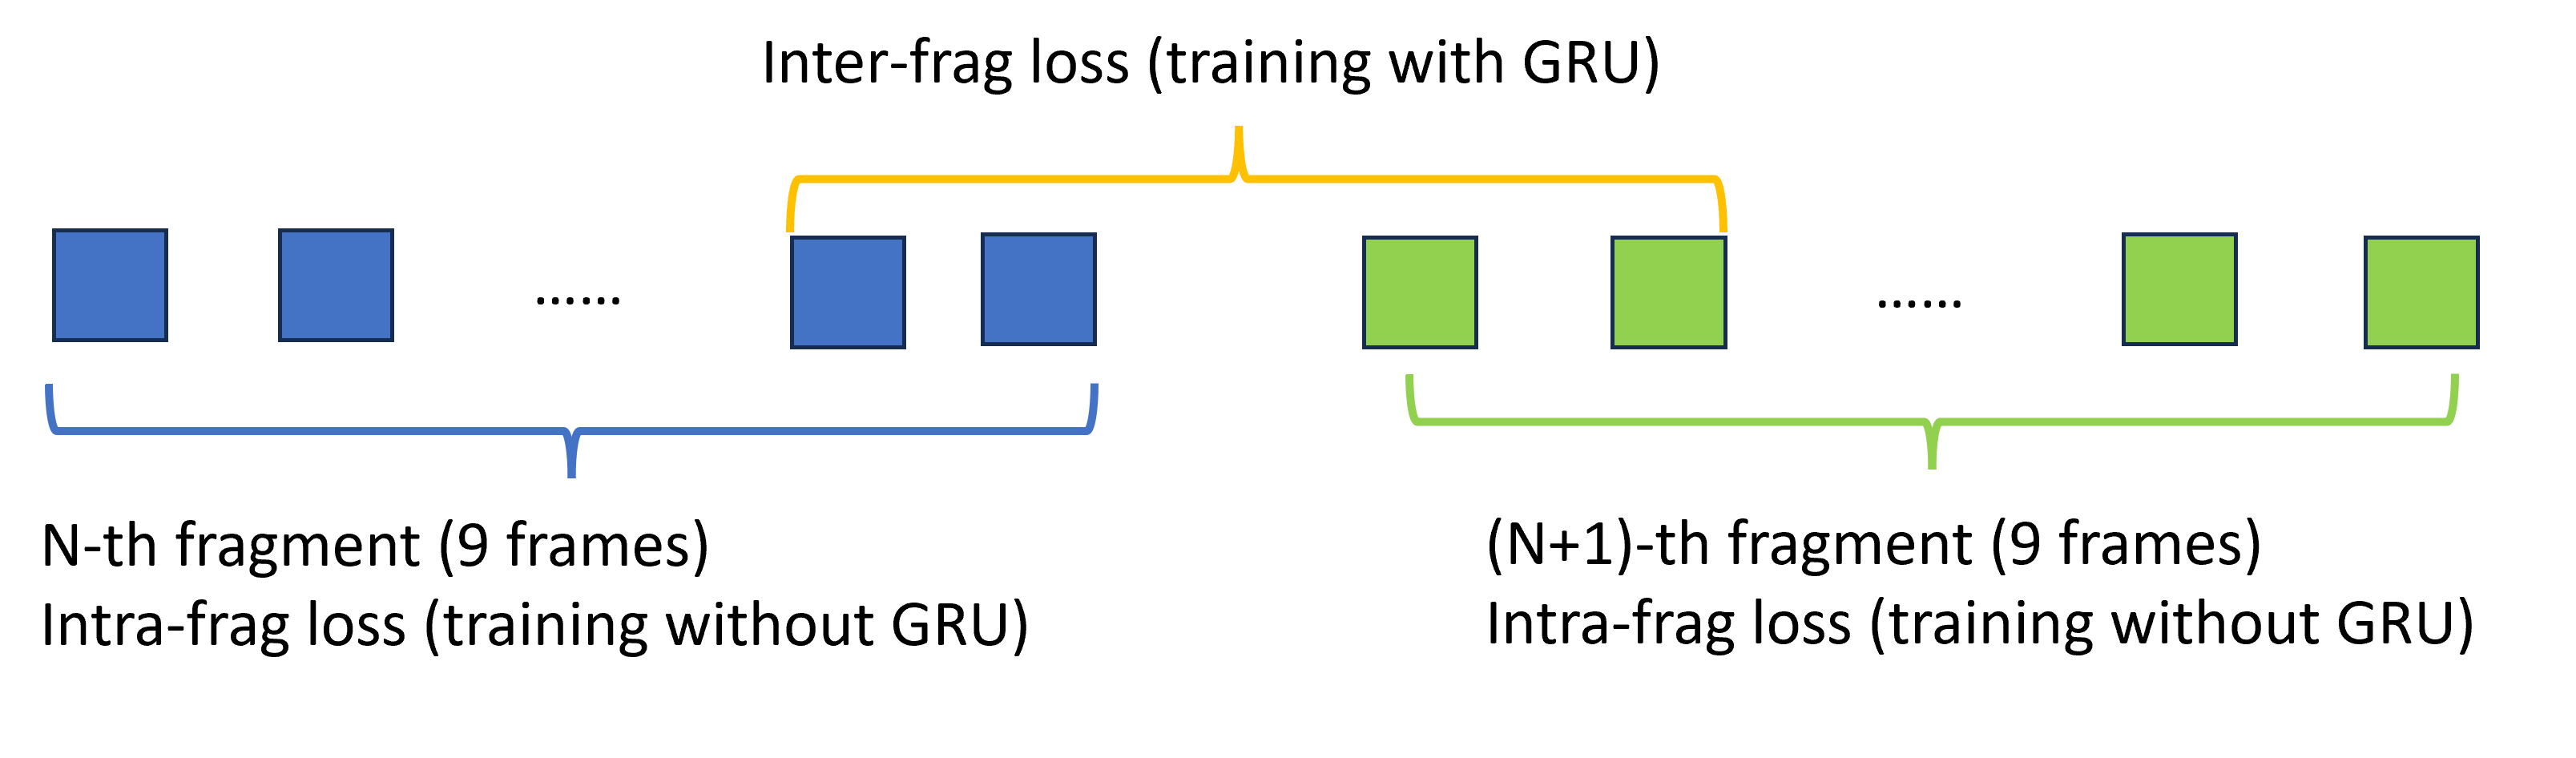
\includegraphics[width=\linewidth]{figures/GRUloss_explain.png}
    \caption{\textbf{Inter/Intra-fragment} losses illustration.}
    \label{fig:gruloss_explain}
\end{figure}


\subsection{NeRF}

\begin{figure}
    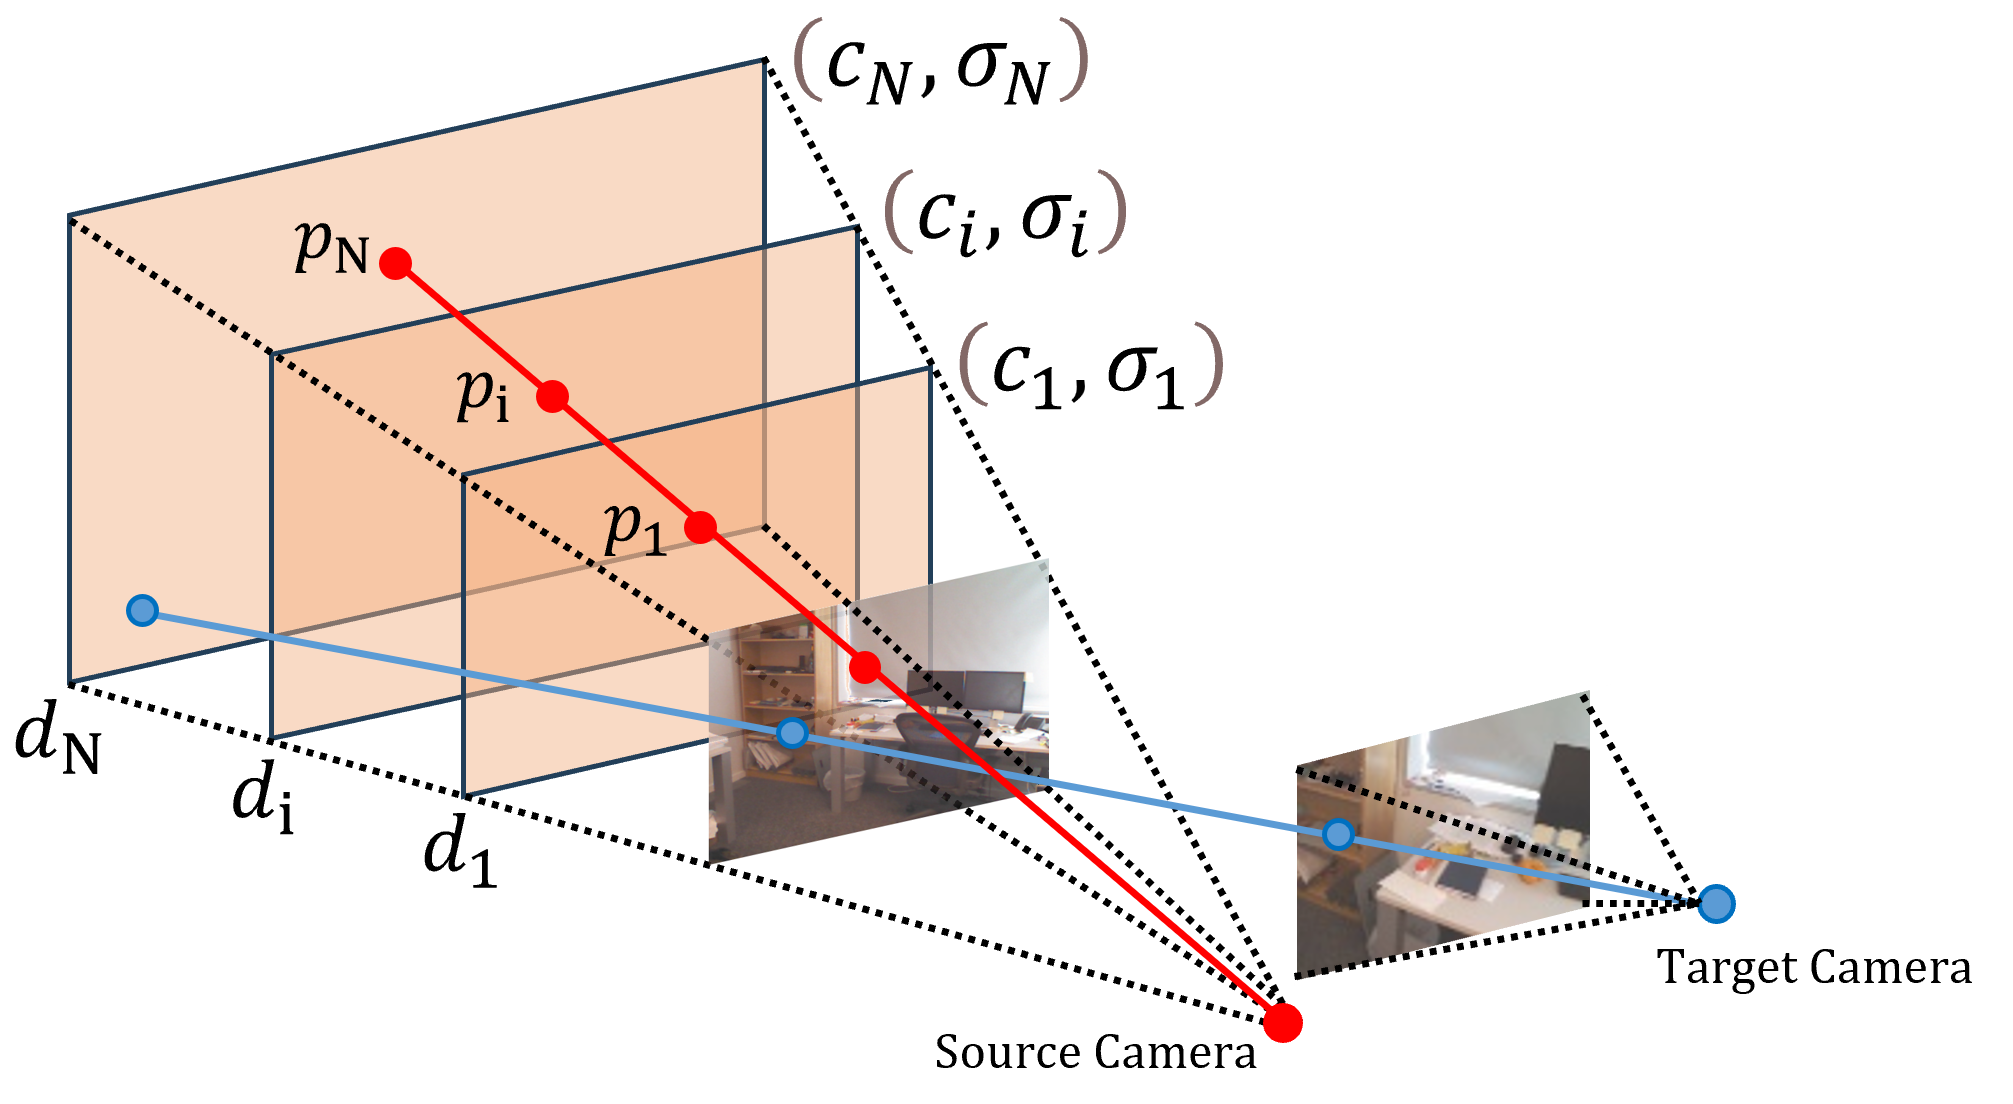
\includegraphics[width=\linewidth]{figures/MPI_explain.png}
    \caption{\textbf{Multi-Plane Image (MPI)} NeRF illustration.}
    \label{fig:mpi_explain}
\end{figure}


Since the SDF decoder is generalizable, the NeRF also must be generalizable to boost SDF decoder. For our work, we adopted MPI-NeRF\cite{mpi, mpi-nerf}, which has been directly used by MonoNeRF\cite{mononerf} and proved to be generalizable. As Figure \ref{fig:mpi_explain} shows, in Multi-Plane-Image (MPI) system, an image is represented by a set of parallel planes (orange planes) denoted as RGB-$\sigma$, specifically $(c_{i}, \sigma_{i})_{i=1}^N$,  where the $i_{th}$ plane has $d_{i}$ disparity (reverse of depth) to the camera. The shading points (red points) are selected as the intersection of the parallel planes and the rays shooting from pixels in the image, where $c_{i}$ and $\sigma_{i}$ are the RGB color and density of each shading points at $i_{th}$ plane. In a standard MPI system, the source view RGB image $\hat{I_{s}}$ and depth map $\hat{D_{}}$ can be composed using the ``over'' operation \cite{over_composite} as

\iffalse
\begin{equation}
    \Biggl\{ \begin{array}{cc}
     \hat{I}_{s} = \sum_{i=1}^{D}(c_{i}\sigma_{i}\prod_{j=i+1}^{D}(1-\sigma_{j})) \\
     \\
     \hat{D}_{s} = \sum_{i=1}^{D}(d_{i}^{-1}\sigma_{i}\prod_{j=i+1}^{D}(1-\sigma_{j}))
     \end{array}
\end{equation}
\fi


{
\begin{equation}
\begin{aligned}
    \hat{I}_s &= \sum_{i=1}^{D} (c_i \sigma_i \prod_{j=i+1}^{D} (1 - \sigma_j)) \\
    \hat{D}_s &= \sum_{i=1}^{D} (d_i^{-1} \sigma_i \prod_{j=i+1}^{D} (1 - \sigma_j))
\end{aligned}
\label{eq:combined}
\end{equation}
}

To use MPI system in NeRF style, the composition operation above can be replaced by volumetric rendering \cite{nerf} for both RGB and depth as 
\iffalse
\begin{equation}
    \Biggl\{ \begin{array}{cc}
    \hat{I_s} = \sum_{i=1}^{N}T_{i}(1-exp(-\sigma_{i}\delta_{i}))c_{i} \\
    \\
    \hat{Z_s} = \sum_{i=1}^{N}T_{i}(1-exp(-\sigma_{i}\delta_{i}))z_{i}
    \end{array}
\end{equation}
\fi

{
\begin{equation}
\begin{aligned}
    \hat{I}_s &= \sum_{i=1}^{N}T_{i}(1-exp(-\sigma_{i}\delta_{i}))c_{i} \\
    \hat{Z}_s &= \sum_{i=1}^{N}T_{i}(1-exp(-\sigma_{i}\delta_{i}))z_{i}
\end{aligned}
\label{eq:combined}
\end{equation}
}

\noindent where $z_i$ is the rendered depth (reverse of disparity) $z_i = 1/d_i$, and $\delta_i = ||p_{i+1} - p_i||_2$ is the distance between the two neighbor shading points on a ray. Then we can extend volumetric rendering to target views. First, the corresponding pixels $[u_t, v_t]$ in the target view can be found by 

\begin{equation}
    \begin{bmatrix}
        u_{s} \\
        v_{s} \\
        1
    \end{bmatrix}
    \sim K_{s}(R-tn^{T}d_{i})(K_{t})^{-1}
    \begin{bmatrix}
        u_{t} \\
        v_{t} \\
        1
    \end{bmatrix}
\end{equation}

Here, $[u_s, v_s]$ is the corresponding pixel locations in the source view, $K_s$ and $K_t$ are camera intrinsics of source and target views, $R$ and $t$ are rotation and translation from the target to source view, and $n$ is the norm vector of the $i_{th}$ plane. As the planes are parallel, the RGB $c'_i$ and density $\sigma'_i$ of shading points (blue points) on target rays (blue ray) are equal to those from source rays at the same disparity, as shown in Eq. \ref{mpinerf_samergbsigma},

\iffalse
\begin{equation}
    \Biggl\{ \begin{array}{cc}
    c_{i}'(u_{t}, v_{t}) = c_{i}(u_{s}, v_{s}) \\
    \sigma_{i}'(u_{t}, v_{t}) = \sigma_{i}(u_{s}, v_{s})
    \end{array}
    \label{mpinerf_samergbsigma}
\end{equation}
\fi

{
\begin{equation}
\begin{aligned}
    c_{i}'(u_{t}, v_{t}) = c_{i}(u_{s}, v_{s}) \\
    \sigma_{i}'(u_{t}, v_{t}) = \sigma_{i}(u_{s}, v_{s})
\end{aligned}
\label{mpinerf_samergbsigma}
\end{equation}
}

\iffalse
\begin{equation}
    \Biggl\{ \begin{array}{cc}
     \hat{I}_{t} = \sum_{i=1}^{D}(c_{i}'\sigma'_{i}\prod_{j=i+1}^{D}(1-\sigma_{j}')) \\
     \\
     \hat{D}_{t} = \sum_{i=1}^{D}(d_{i}\sigma'_{i}\prod_{j=i+1}^{D}(1-\sigma_{j}'))
     \end{array}
\end{equation}
\fi

Once we have RGB and density for target views, we can perform volumetric rendering on target views as: 
\iffalse
\begin{equation}
    \Biggl\{ \begin{array}{cc}
    \hat{I_t} = \sum_{i=1}^{N}T_{i}(1-exp(-\sigma'_{i}\delta_{i}))c'_{i} \\
    \\
    \hat{Z_t} = \sum_{i=1}^{N}T_{i}(1-exp(-\sigma'_{i}\delta_{i}))z'_{i}
    \end{array}
\end{equation}
\fi

{
\begin{equation}
\begin{aligned}
    \hat{I_t} = \sum_{i=1}^{N}T_{i}(1-exp(-\sigma'_{i}\delta_{i}))c'_{i} \\
    \hat{Z_t} = \sum_{i=1}^{N}T_{i}(1-exp(-\sigma'_{i}\delta_{i}))z'_{i}
\end{aligned}
\label{eq:combined}
\end{equation}
}

We use standard NeRF RGB loss, where $\hat{I}_s$ and $\hat{I}_t$ are self-supervised with their corresponding input images with a L1 loss. Since we directly use the reverse of disparity for depth, the depth value is scale-ambiguous. As mentioned in the paper, since there is no depth ground truth for pure self-supervision, we use SDF-depth as pseudo-depth to first recover the real scale of $\hat{Z}_s$ and $\hat{Z}_t$, then we impose a consistency loss between $\hat{Z}$ and SDF-depth to boost SDF decoder.

    

\section{Visual Results}
We show more visual results of 2D rendered depth and 3D mesh in Figure \ref{fig:scannet_supp}. \textbf{We also attach a PowerPoint file with visual results, where reviewers can rotate and zoom the 3D mesh to see the details},

\section{Limitation}
Although our work combines the advantages of ``self-supervised'' ``generalizable'' and ``3D explicit mesh'' altogether, there are still limitations. So far our MonoSelfRecon can be only used for indoor environments, because we pre-define the 3D scene fragment with a fixed voxel number. Unlike indoor 2D images where depth vary within few meters, the depth can vary significantly just within a single 2D image in outdoor. It is applicable to keep the voxel number while increasing the voxel size, but it will lead to very poor resolution within voxels, which misses most of the details. Moreover, since we regress SDF corresponding to the discrete $N\times N\times N$ voxels of scene fragment, we cannot directly estimate SDF of a continuous 3D space, unless by interpolation. By contrast, SDF-NeRF based methods estimate SDF values in continuous 3D space but it is not generalizable to another scene. Our future works will explore to make SDF-NeRF generalizable, so that the 3DR can be ``self-supervised", ``generalizable", ``explicit'', ``indoor/outdoor'', and ``continous in 3D space''. 

\newpage
\begin{figure*}
\begin{minipage}{\textwidth}
  \centerline{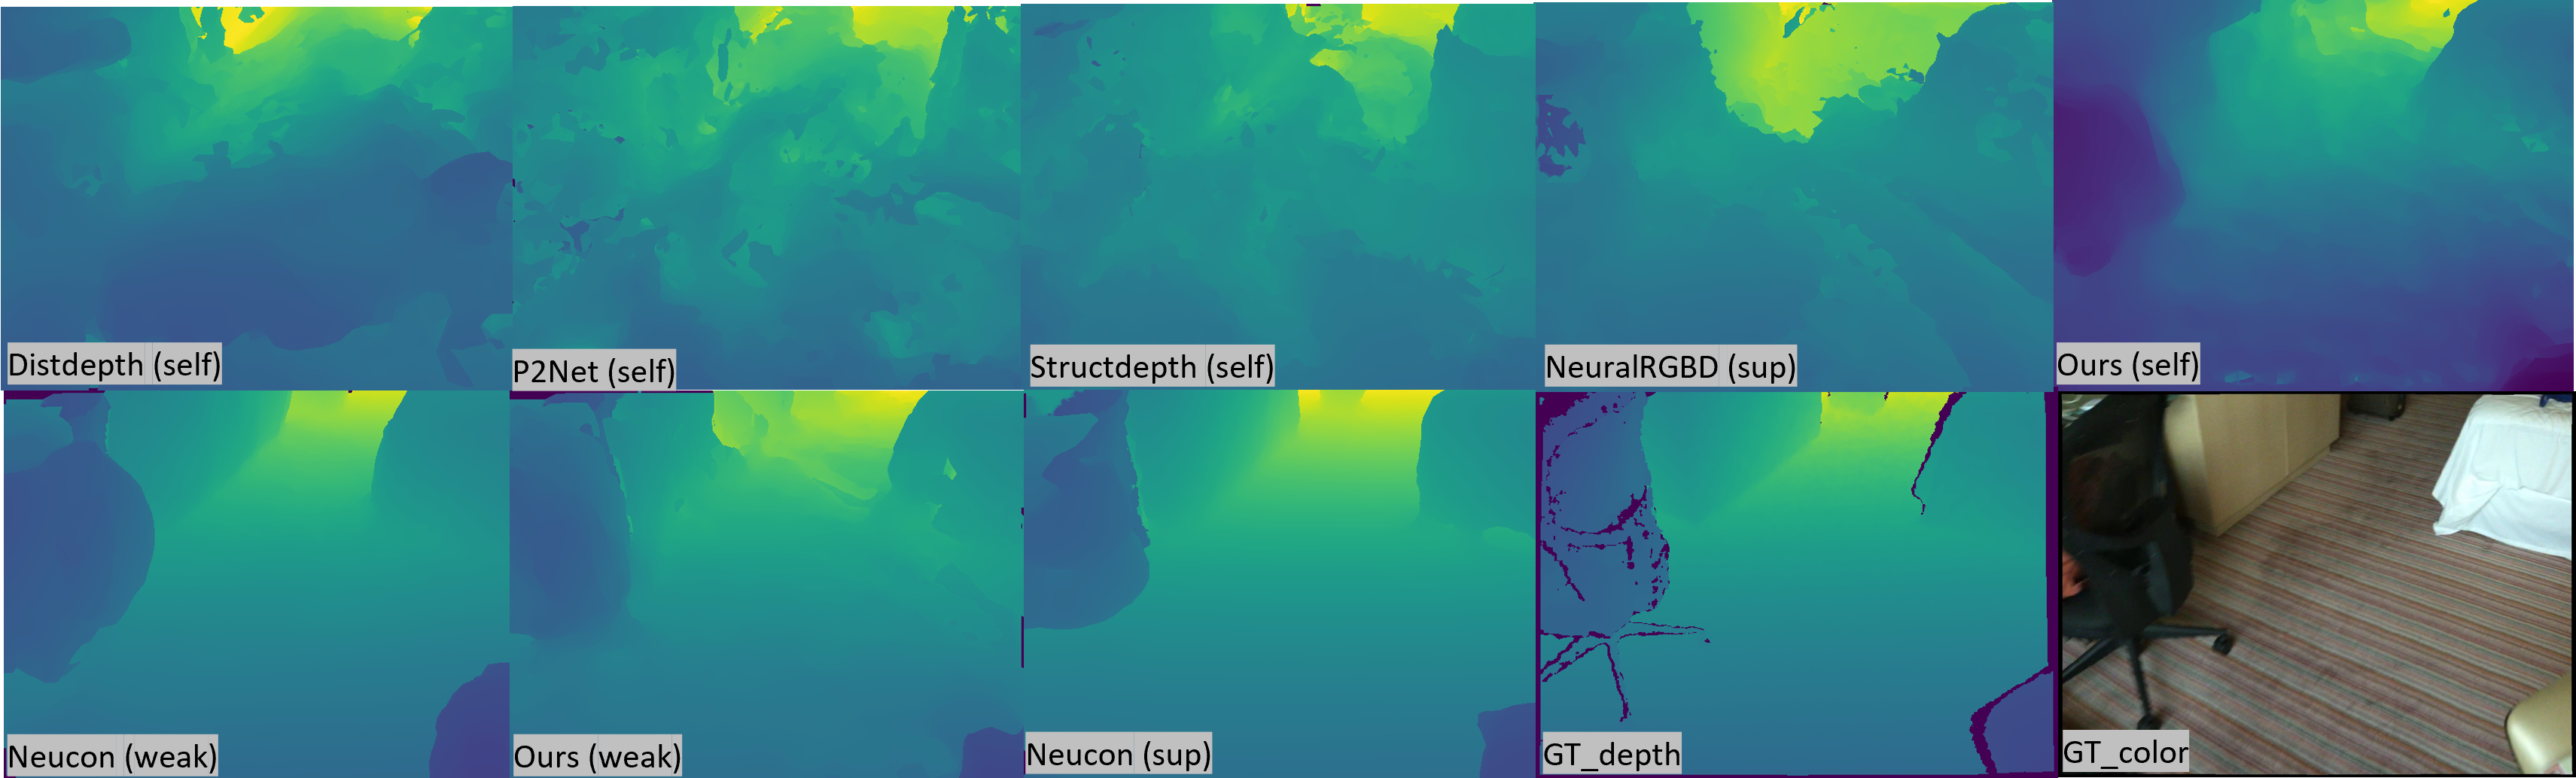
\includegraphics[width=1.0\textwidth]{figures/scannet_depth/738_1300.png}}
\end{minipage}
\vfill
\begin{minipage}{\linewidth}
  \centerline{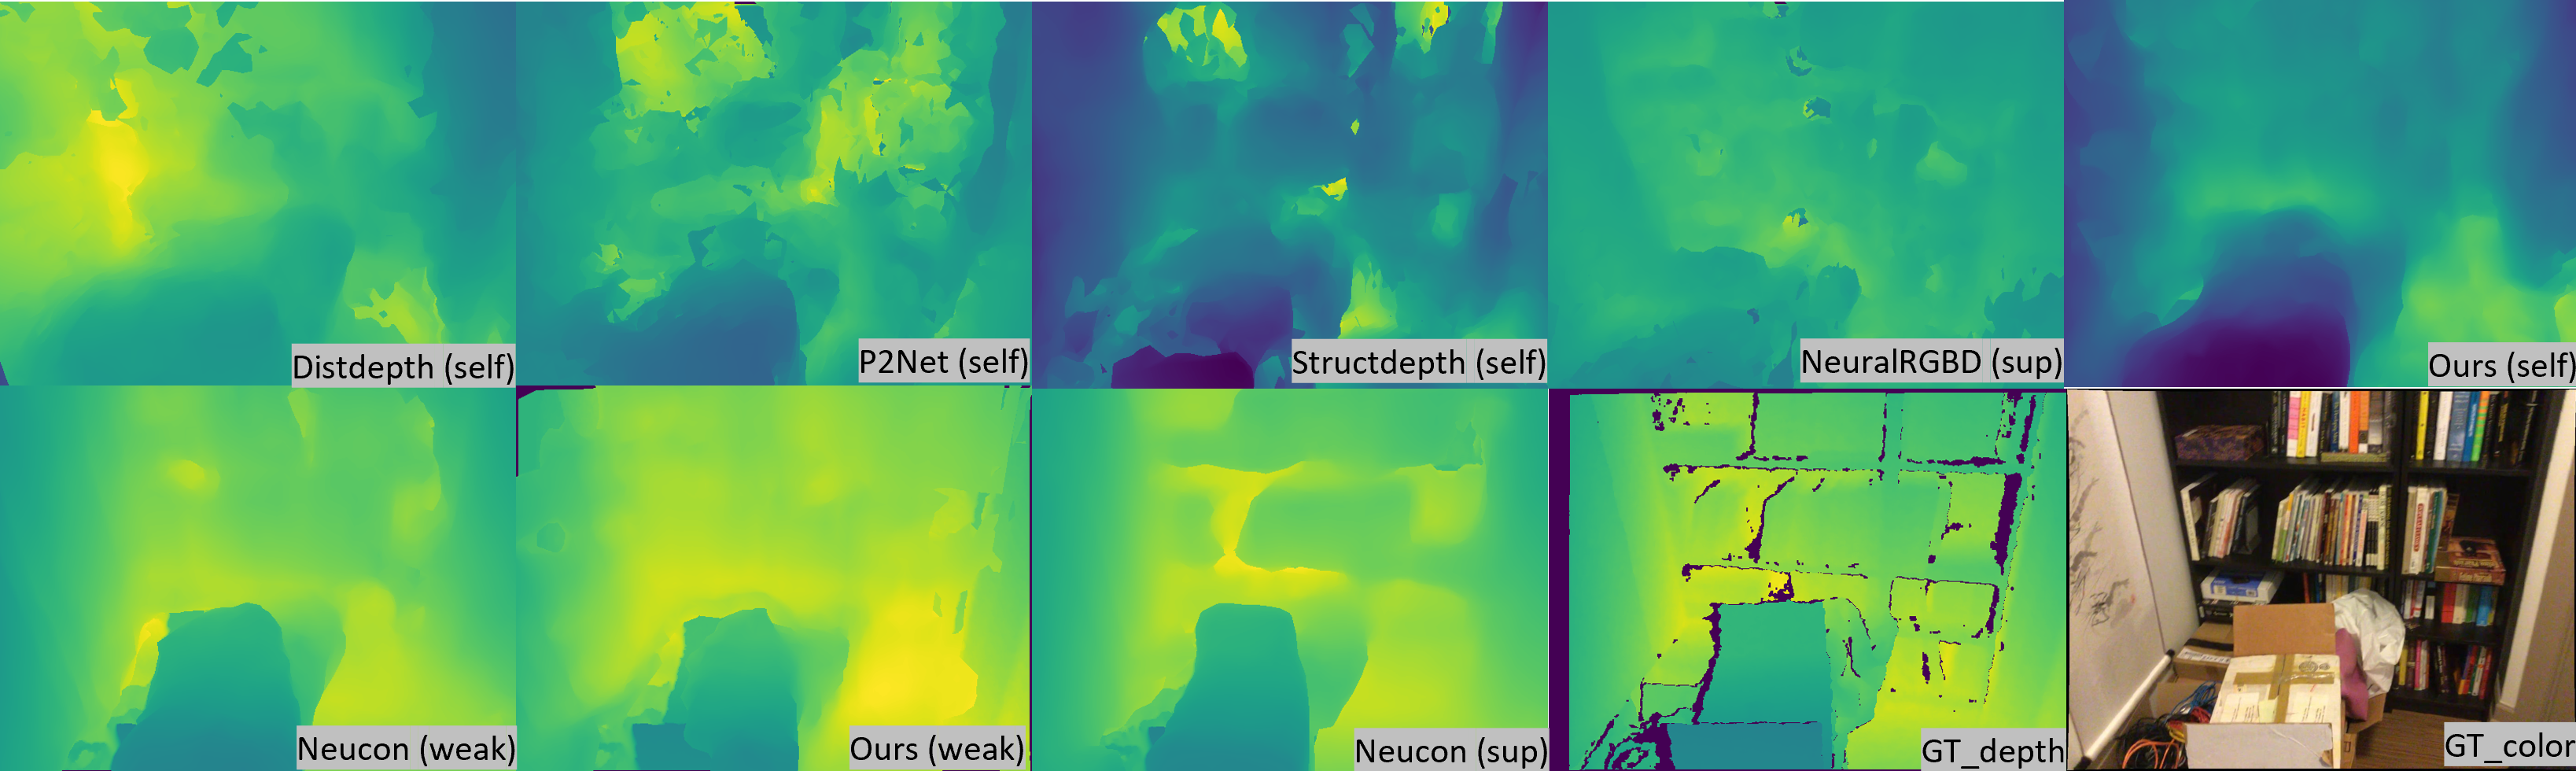
\includegraphics[width=1.0\textwidth]{figures/scannet_depth/710_1210.png}}
\end{minipage}
\vfill
\begin{minipage}{\linewidth}
  \centerline{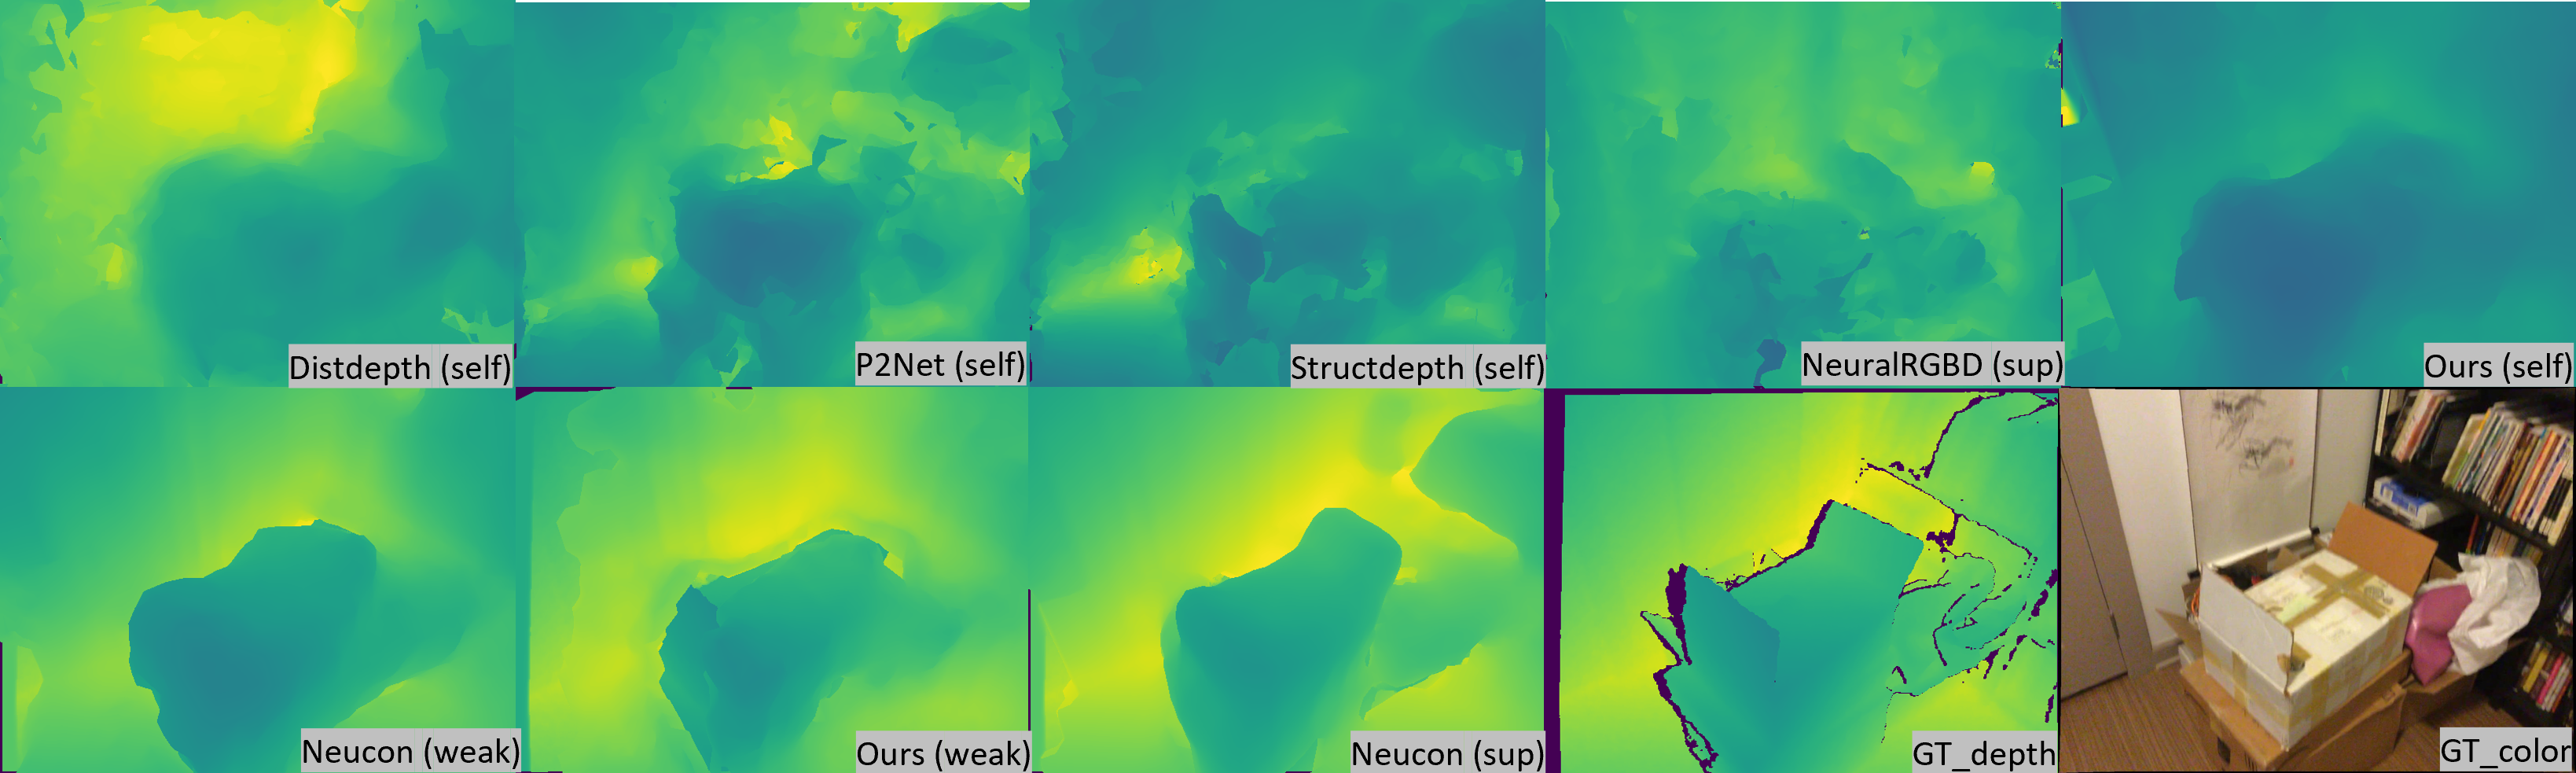
\includegraphics[width=1.0\textwidth]{figures/scannet_depth/710_1280.png}}
\end{minipage}
%\vspace{-3mm}
\begin{minipage}{\linewidth}
  \centerline{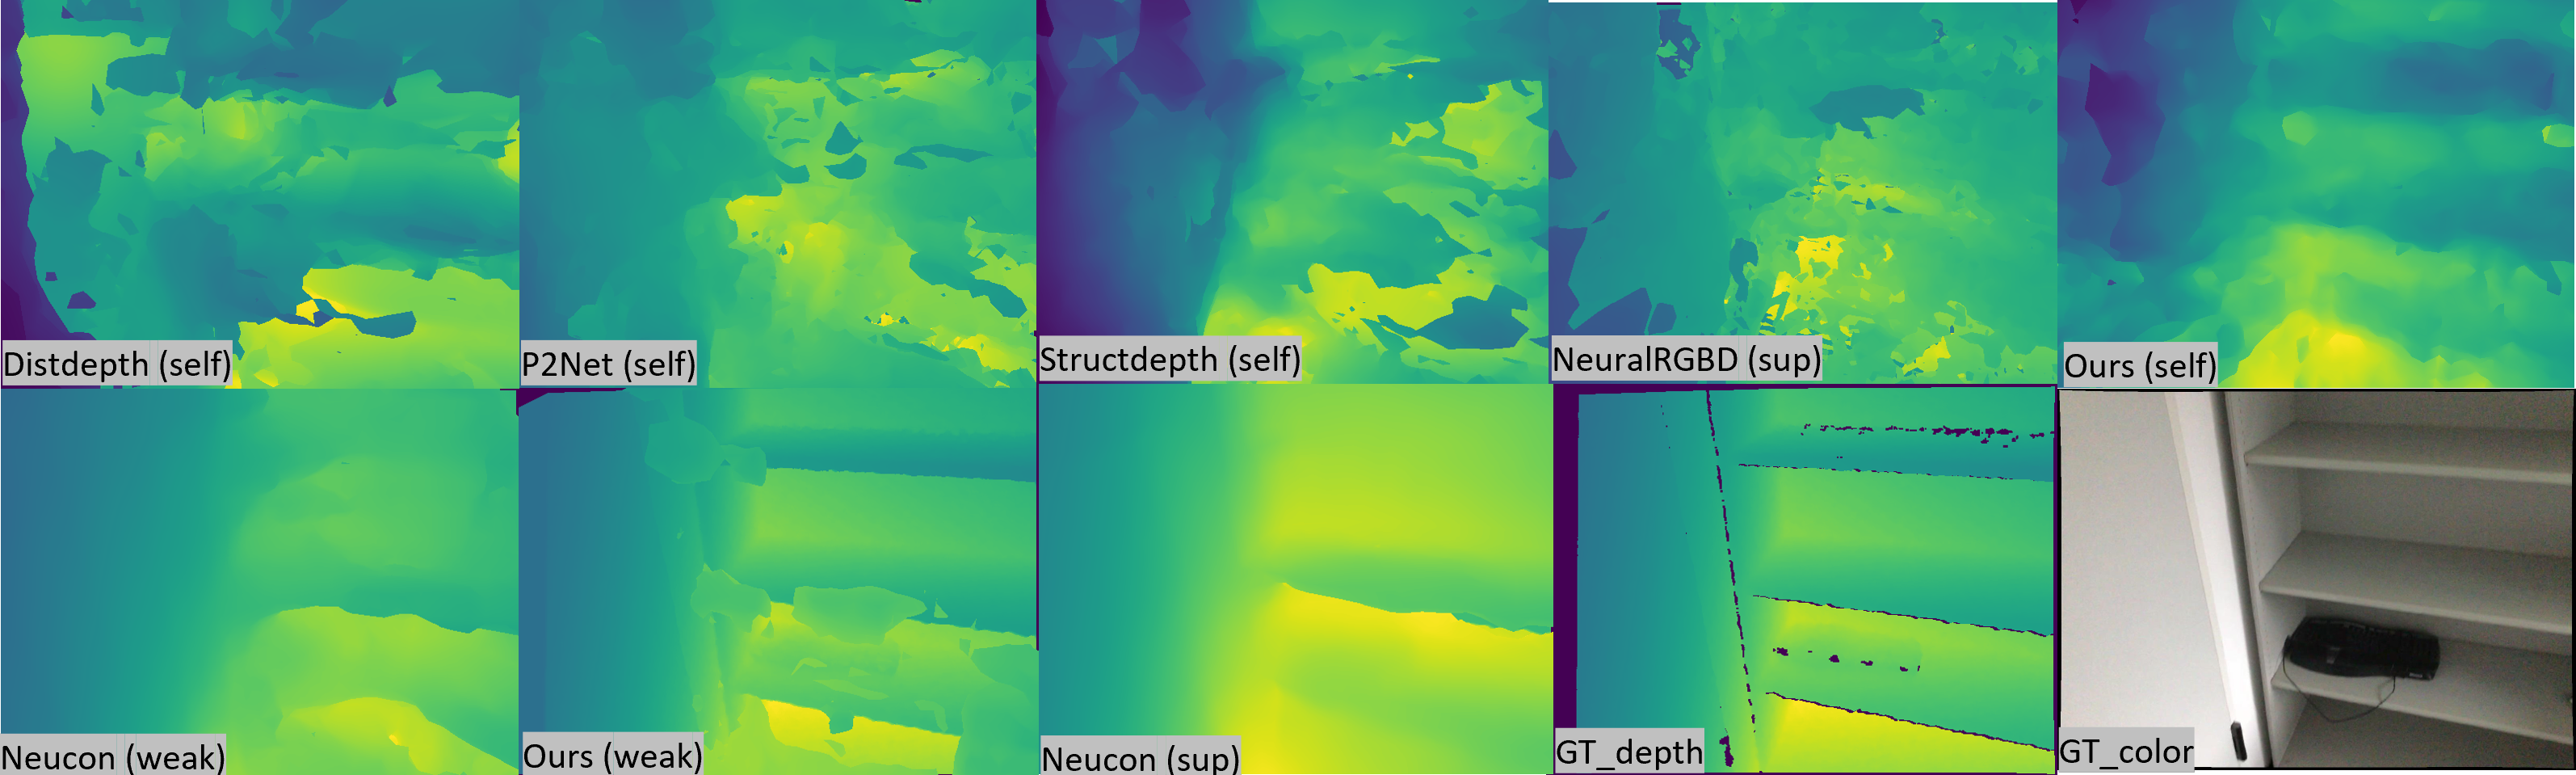
\includegraphics[width=1.0\textwidth]{figures/scannet_depth/711_880.png}}
\end{minipage}
%\vspace{-3mm}
\end{figure*}

\newpage
\begin{figure*}
\begin{minipage}{\textwidth}
  \centerline{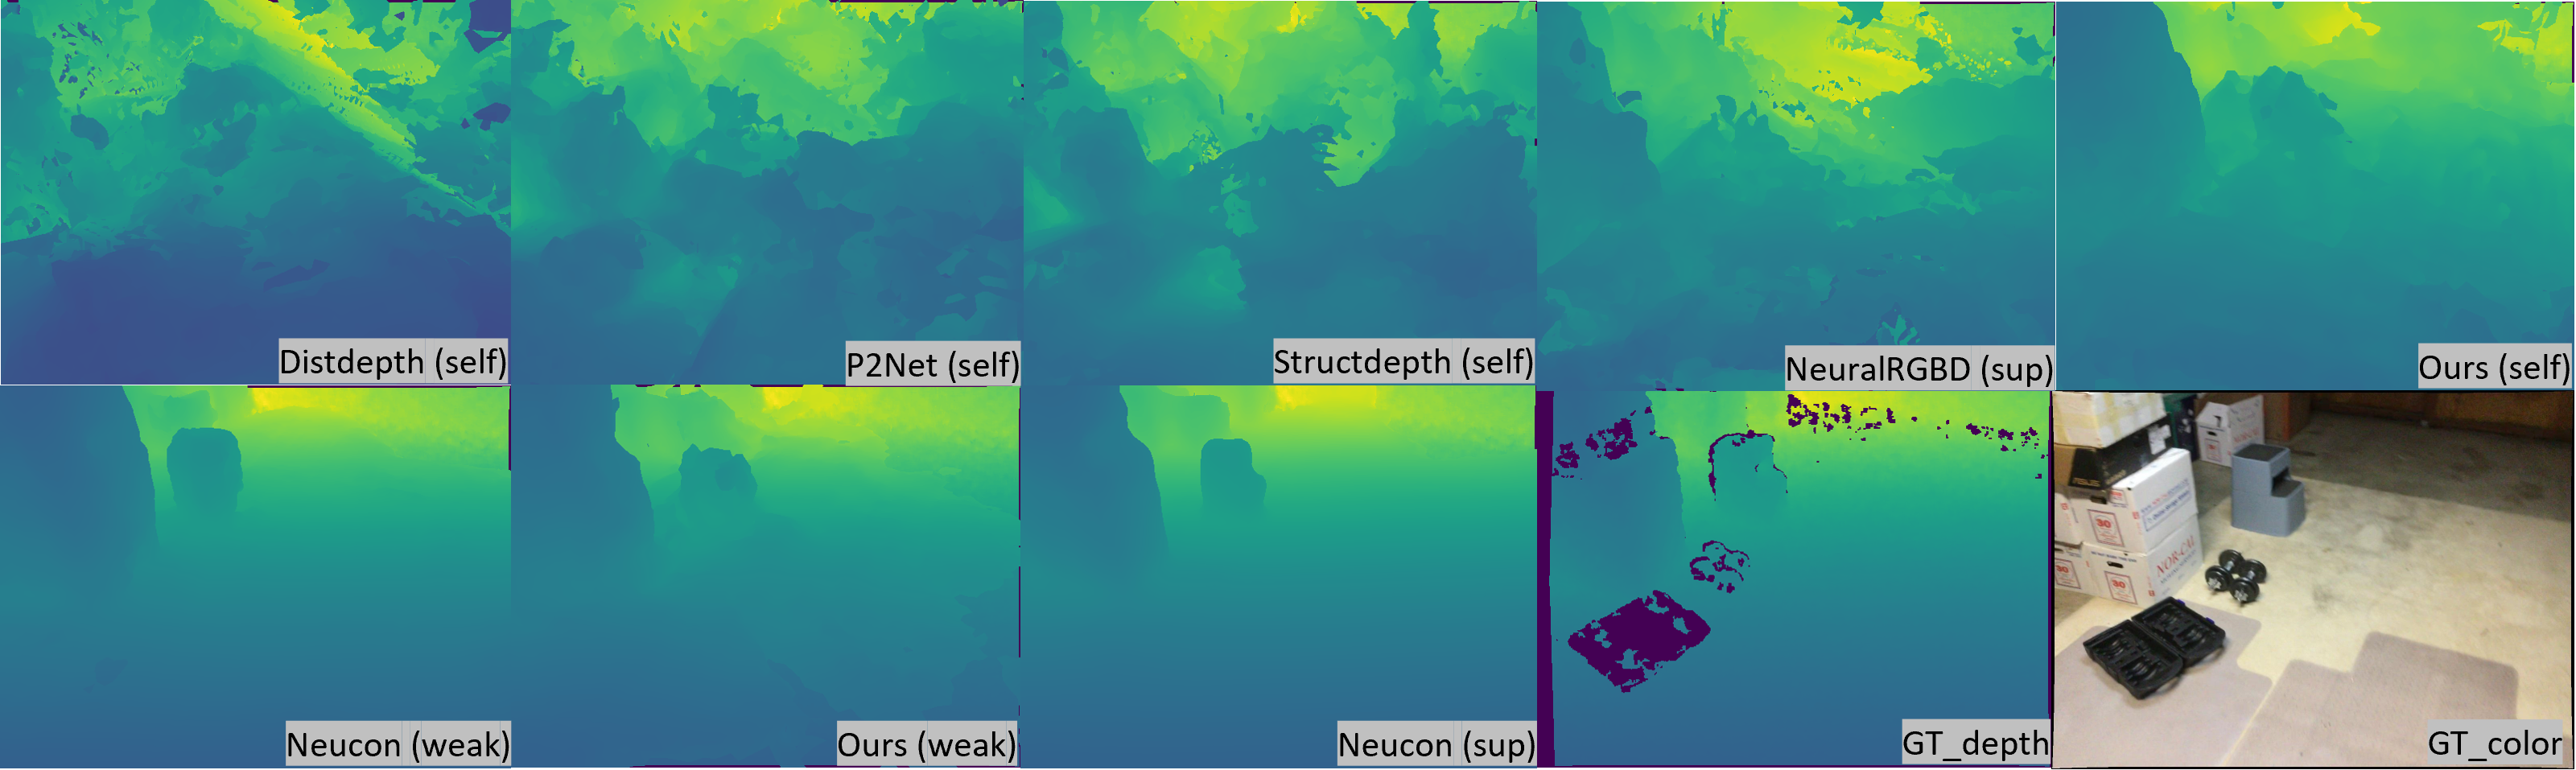
\includegraphics[width=1.0\textwidth]{figures/scannet_depth/787_1720.png}}
\end{minipage}
\vfill
\begin{minipage}{\linewidth}
  \centerline{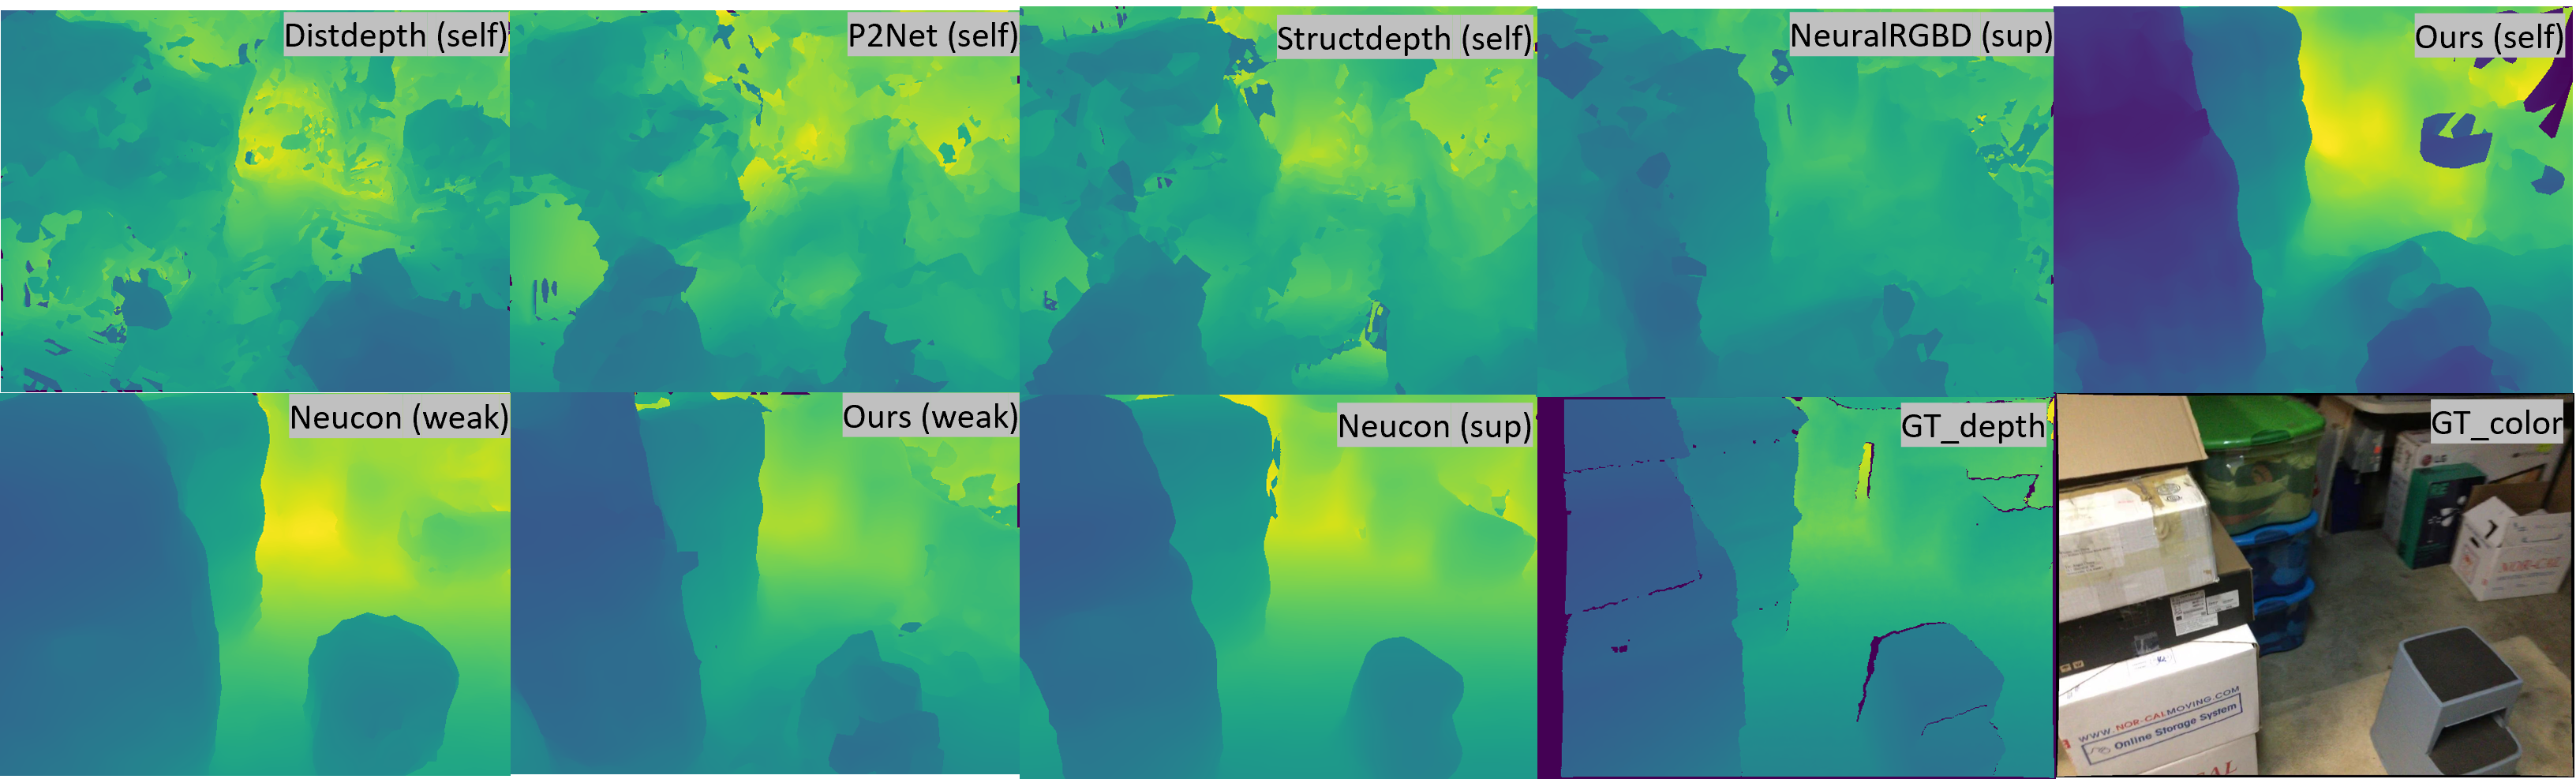
\includegraphics[width=1.0\textwidth]{figures/scannet_depth/787_1930.png}}
\end{minipage}
\vfill
\begin{minipage}{\linewidth}
  \centerline{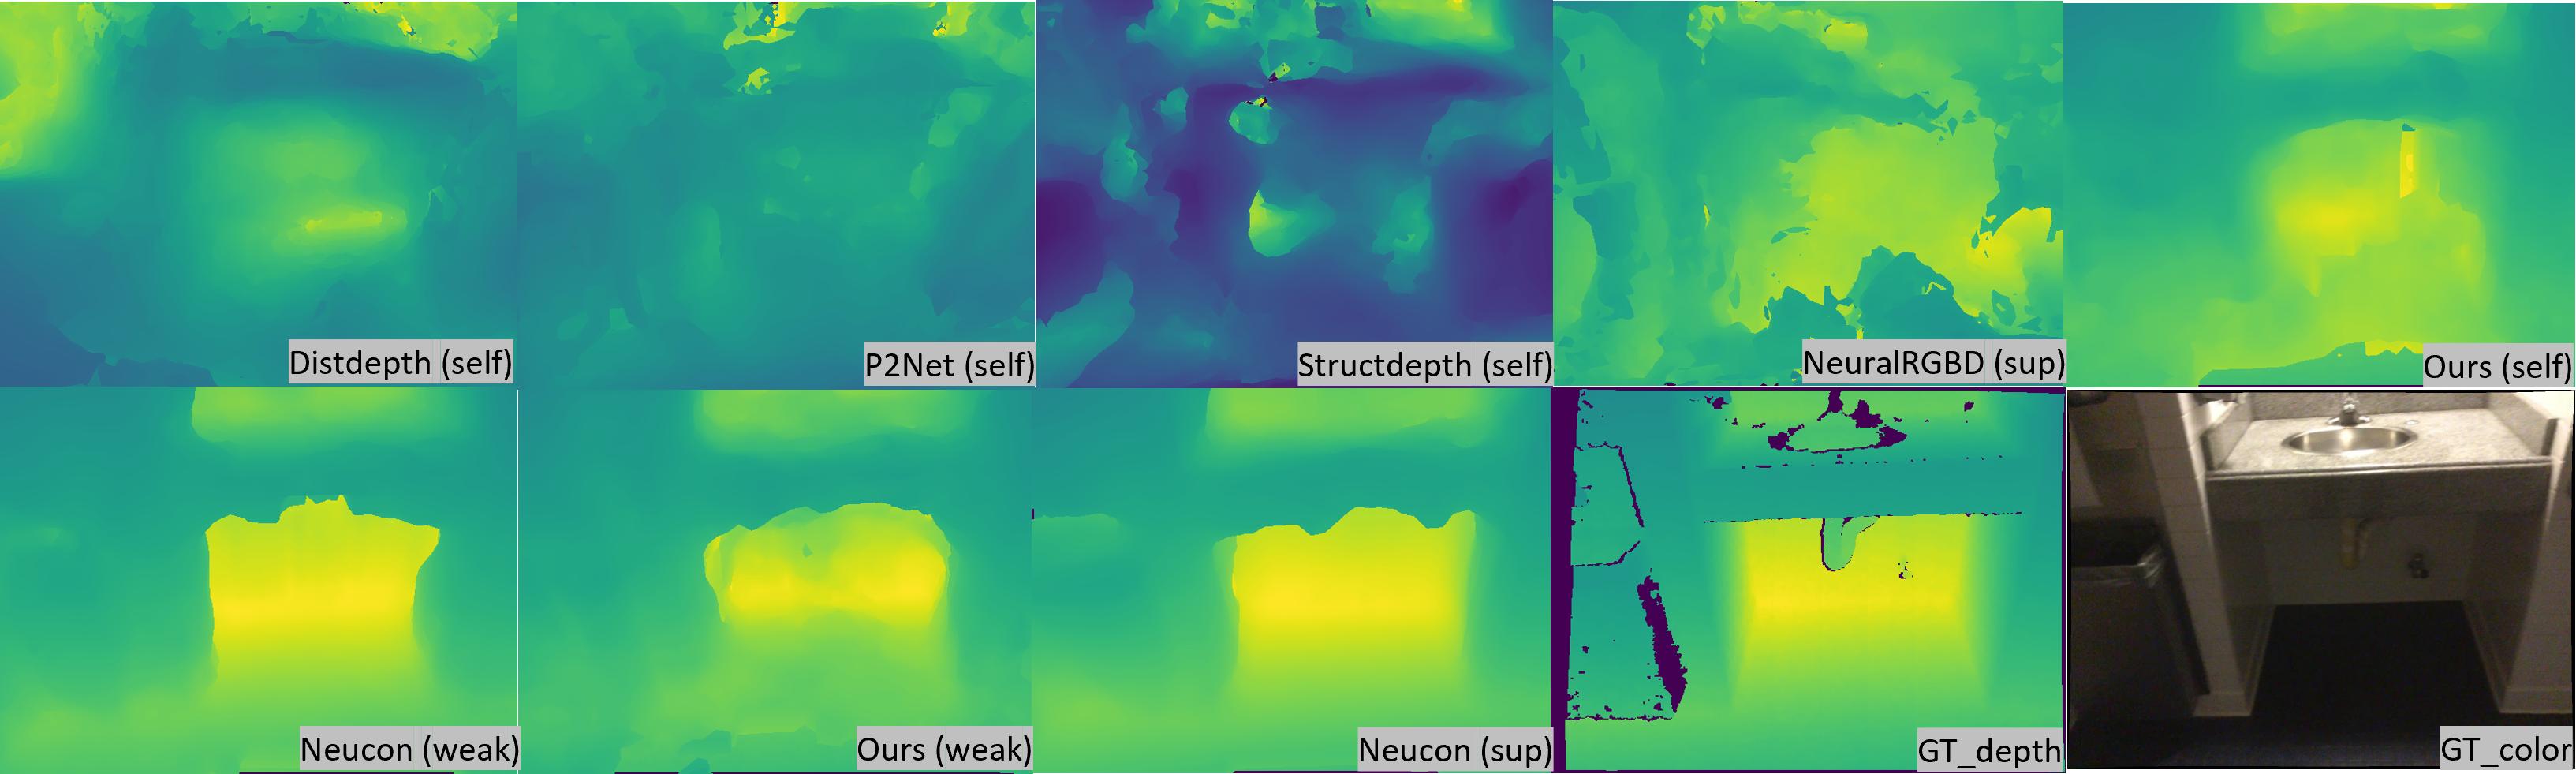
\includegraphics[width=1.0\textwidth]{figures/scannet_depth/779_1125.png}}
\end{minipage}
%\vspace{-3mm}
\begin{minipage}{\linewidth}
  \centerline{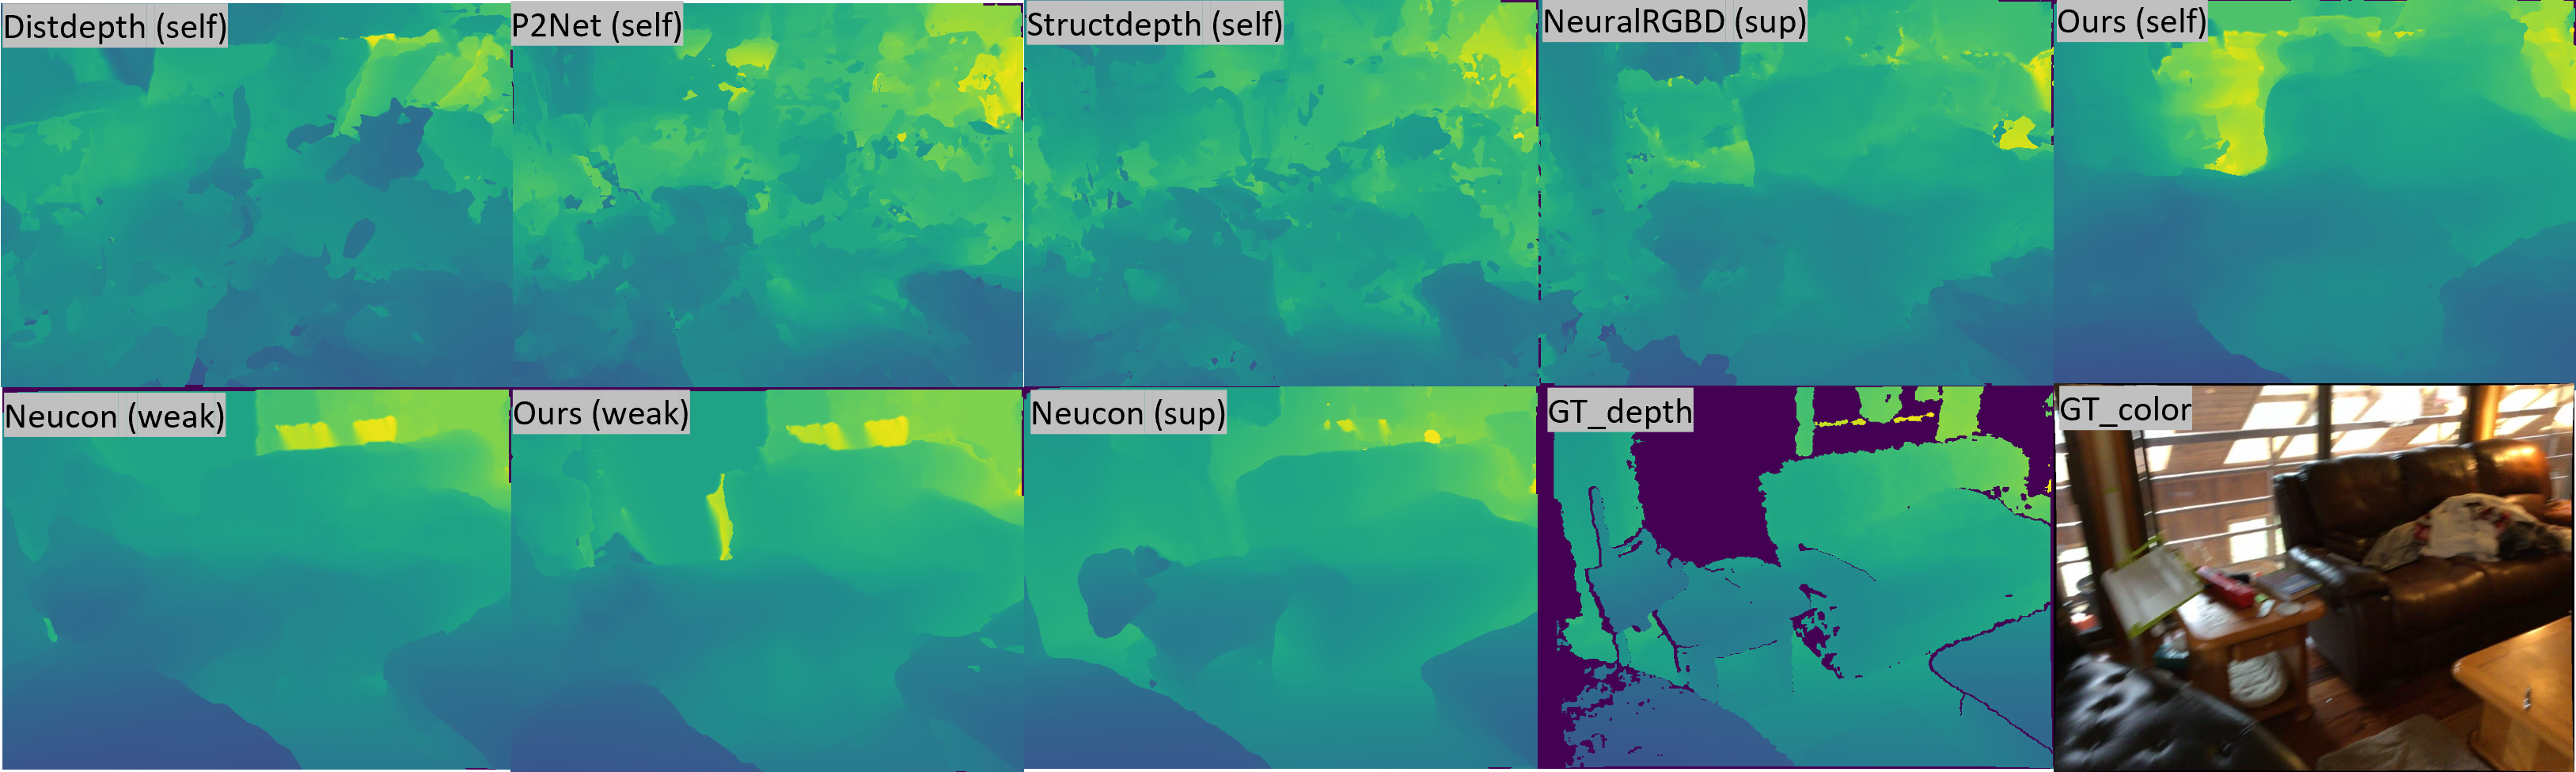
\includegraphics[width=1.0\textwidth]{figures/scannet_depth/747_97.png}}
\end{minipage}
%\vspace{-3mm}
\vspace{-3mm}
\end{figure*}

\newpage
\begin{figure*}
\begin{minipage}{\textwidth}
  \centerline{\includegraphics[width=1.0\textwidth]{figures/scannet_mesh/787.png}}
\end{minipage}
\vfill
\begin{minipage}{\linewidth}
  \centerline{\includegraphics[width=1.0\textwidth]{figures/scannet_mesh/747.png}}
\end{minipage}

\iffalse
\vfill
\begin{minipage}{\linewidth}
  \centerline{\includegraphics[width=1.0\textwidth]{figures/scannet_mesh/710.png}}
\end{minipage}
\fi
\label{fig:scannet_supp}
    \caption{Visual Results}
\end{figure*}


\clearpage 
\appendix


 \clearpage\section*{\Large Supplementary Materials - DGR-MIL: Exploring Diverse Global Representation in Multiple Instance Learning for Whole Slide Image Classification}

\clearpage
\appendix
\section*{Supplementary Material}

This part of the paper is organized as follows:
\begin{itemize}
    \item \cref{appendix:faq} overviews several common questions about the details of our study and addresses the limitations of SWARM parallelism;
    \item In \cref{appendix:related}, we list further related works on topics relevant to the problem setting we study;
    \item In \cref{appendix:wiring_details} and \cref{appendix:rebalancing_formal}, we give a more formal description and outline the details of stochastic wiring and adaptive rebalancing, accordingly;
    \item In \cref{appendix:equivalence}, we outline the relation between training with SWARM and using methods for offloading.
    \item \cref{appendix:detailed_setup} and  \cref{appendix:detailed_large} contain additional details of our experimental setup, whereas \cref{appendix:scaling} reports further experiments on specific aspects and components of SWARM parallelism;
    \item Lastly, we investigate compression-aware architectures in \cref{appendix:compression} and evaluate their impact in a practical setting in \cref{appendix:time_to_solution}.
\end{itemize}

\section{Answers to Common Questions}
\label{appendix:faq}


\paragraph{Why not just use data parallelism with offloading?}

Regular data parallelism requires all-reduce steps where peers exchange gradients, which can be prohibitively expensive for large models. For example, a 1 billion parameter model with 16-bit gradients requires 2 GB of data to be synchronized between all $n$ devices. We need at least $n$ messages to perform this synchronization. If we have 100 devices with bidirectional communication, each client would need to send 2 GB of data to finish the synchronization. Thus, with slow interconnects, such synchronizations are not practical.

\paragraph{Why not just use fully sharded data parallelism with elasticity?}

Sharded data parallelism requires all-to-all communication of parameter buffers at each layer. Each of these communications can be done in parallel and has a size of parameter count divided by $n$; in total, $n$ messages are required. Thus, for 1B parameters in 16-bit precision, a total of 2 GB need to be synchronized for both the forward and backward pass. For low-bandwidth devices with 100 Mb/s speed, this would entail an overhead of 5.5 minutes per forward/backward pass, which is difficult to overlap with computation. This is exacerbated further, because all-to-all communication latency is determined by the slowest peer. Thus, sharded data parallelism can be particularly inefficient for setups where peers have different network bandwidths.

\paragraph{Should I use SWARM in a supercomputer?}
By default, SWARM is worse than traditional parallelism due to its extra complexity (see experiments in Section~\ref{appendix:training_throughput}). However, SWARM can be useful in case of supercomputers that have heterogeneous devices.

\paragraph{ZeRO-Offload allows one to train 13B parameters on a single V100, so why do I need SWARM?}

Using ZeRO-Offload can slow down training due to the slow data transfer between external memory and the accelerator. Training with SWARM can {\it accelerate} training while also allowing to train larger models; see Appendix~\ref{appendix:equivalence} for a detailed comparison.

\paragraph{Is it worth using preemptible instances and SWARM from an economic standpoint?}
Due to a significantly smaller cost per hour, one can leverage a larger amount of computation when using spot instances compared to on-demand cloud VMs or dedicated HPC setups. See \autoref{appendix:time_to_solution} and \autoref{tab:cost} for a comparison of both hourly and total costs for an example large-scale pretraining task.

\paragraph{When should I avoid using SWARM?}

SWARM is efficient at training compute-intensive models with more than 1B parameters. For smaller models, a sharded data-parallel approach can be more optimal. For homogeneous HPC environments, standard sharded data-parallel or pipeline-parallel training will be more efficient than SWARM, because the rebalancing is not required. For HPC environments that are so extensive that the failure of a node is likely, the practicality of SWARM depends on how many nodes are expected to fail. Elastic sharded data parallelism is better than SWARM if the number of expected failures is relatively low.

\paragraph{Can I use SWARM without layer sharing or quantization?}
Yes, SWARM can still be effective in these scenarios. Our bandwidth experiments in the main part of the work give an estimate of its network overhead. By using no quantization, which means using regular 16-bit activations, the network overhead increases approximately by a factor of two. Without layer sharing, the overhead within each pipeline stage to synchronize the gradients is increased by the number of layers not being shared. As such, a rough estimate of the efficiency of SWARM in these scenarios can be estimated by taking our model size and network bandwidth requirements data and multiplying it by the relevant factor.

\paragraph{Do the compression-aware architecture modifications apply only to Transformers?} 
Bottleneck and maxout compression are general compression techniques that can be applied to any layer in any architecture. However, their effectiveness may vary depending on where in the model they are applied and what kind of model these are applied to (for example, CNNs vs. RNNs vs. Transformers).

\paragraph{How many pipeline stages can SWARM have?}
While its design allows for any number of stages, using long pipelines can result in a reduced training throughput. Similarly to regular pipeline parallelism, SWARM suffers from the pipeline ``bubble'' problem~\citep{huang2019gpipe}: at the beginning of the initial batch processing, peers near the end of the pipeline will be waiting for inputs. Likewise, early layers will be idle after processing the final microbatch.
In theory, this can be mitigated with asynchronous updates~\citep{pipedream,pipemare}, but we did not investigate them in this work due to potential convergence issues.

\paragraph{How much failure can SWARM handle?}
As long as there is at least one operational peer at every pipeline stage and at least one trainer, SWARM can work without any issues. 
The key factors defining the training run state at a given SGD step are the model parameters, the optimizer statistics, the data loader state, and the step number (required for proper scheduling). The up-to-date parameters and optimizer statistics, as well as the step number, are naturally located on all active nodes of a given stage, since they are required for training. Thus, when a peer joins the network, it can download the checkpoint corresponding to the current training state from other peers.

As we mention in Section~\ref{sect:method_swarm}, peer failures do not affect forward and backward passes as long as there is at least one peer at the required stage: because of rewiring, it is possible to resend activations or gradients to another worker that has identical model weights by construction. Similarly, the data loader state can be recomputed from the last known SGD step. However, we do not track the order of examples sampled within the same batch; because of the i.i.d. assumption in the large-scale training setup, the distribution of gradients is expected to be the same. Hence, if the peer leaves from the pipeline stage, other workers can compute gradients and replace those accumulated by the disconnected peer, so that the number of examples for an SGD step stays the same.

\paragraph{Some configurations in Section~\ref{sect:experiments_square_cube} measure less than $\bf 20\%$ GPU idle time, while many HPC systems only achieve $\bf \approx80\%$ GPU utilization. Does this mean that SWARM is $\bf 30\%$ faster?} 
No, because these are different measurement types. \citet{megatron2} measures GPU utilization as a fraction of theoretical peak FLOP/s of their GPUs. In contrast, we only measure what fraction of time the GPU is running the model, regardless of efficiency. Since any realistic deep learning workload cannot achieve $100\%$ peak FLOP/s, $20\%$ GPU idle time for SWARM means that it can reach $\approx0.8$x the training throughput compared to training with an infinitely fast network. As a rule of thumb, one can say that SWARM will run at a $20\%$ slower speed than systems described by~\citet{megatron2} using the infrastructure that is several times cheaper.%


   



\section{Additional Related Work}\label{appendix:related}


\vspace{-2pt}
\paragraph{Dynamic parameter loading.} Several recent studies propose alternative execution algorithms that allow training large models with data parallelism. Since neural networks typically use a small fraction of weights at any given moment, the remaining ``inactive'' parameters can be sharded~\citep{zero} or offloaded to external memory~\citep{l2l,zerooffload,zero_ssd}. In sharded data parallelism~\cite{zero}, inactive tensors are distributed across all $n$ devices such that each device stores $\frac{1}{n}$th of all parameters. For active layers, the shards are gathered such that each device holds the entire tensor just-in-time for computation. After the computation, the parameters' memory is freed so that only the sharded memory remains ($\frac{1}{n}$th per device). This makes it very memory efficient to store model and optimizer states for inactive layers if many devices are available. Similarly to tensor parallelism, these algorithms can support arbitrary models without the need for layer partitioning and can, in principle, run a large model on a single GPU, which is useful for finetuning and inference.

\vspace{-6pt}
\paragraph{Architecture-specific methods.} Finally, some distributed training algorithms take advantage of specific layers, such as locally connected layers~\citep{dean12,coates13}, Mixture-of-Experts~\citep{moe_first,shazeer2017outrageously,Lepikhin2020GShardSG}, Switch layers~\citep{fedus2021switch} or Product Key Memory~\citep{pkm}. These layers contain many near-independent parts that can be assigned to different devices. They can easily scale to an extremely large number of parameters with a relatively small increase in compute~\citep{shazeer2017outrageously}. However, they are also less parameter-efficient~\citep{fedus2021switch} and may not apply to all architectures.

\vspace{-6pt}
\paragraph{Optimal scheduling for distributed training.}
When the configuration of each peer is known, it is possible to significantly optimize the pipeline scheduling by going beyond the greedy approach with global optimization techniques~\citep{alpa,piper}, even with heterogeneous hardware~\citep{yuan2022decentralized}.
However, we consider a setup in which this is not possible: preemptible and volunteer peers can join at any point of the experiment, and dynamically rescheduling and orchestrating them in a centralized manner is technically difficult because of the communication and reliability constraints.

\vspace{-6pt}
\paragraph{Elastic training.} To train with a dynamic number of workers, deep learning practitioners have developed elastic training algorithms~\citep{pytorch_elastic,elastic_horovod}. If a worker leaves or fails during training, these algorithms rebalance the load between the remaining nodes and continue the training procedure~\citep{proteus,moshpit}. If new workers join during training, they get the latest model parameters from their peers and train alongside them.

\vspace{-10pt}
\paragraph{Asynchronous training.} Another important problem is distributed training on devices with uneven performance. One way to solve this problem is to use asynchronous training, where nodes compute gradients at their own pace and aggregate them using a parameter server~\citep{recht2011hogwild,volunteer_dl_async} or a decentralized network~\citep{dp_sgd}. This idea allows full utilization of each device, but may reduce the convergence rate due to ``stale'' gradients~\citep{recht2011hogwild,aji2019making}. Several studies~\citep{wagma,moshpit,zerooffload,dedloc} propose hybrid techniques that remove some synchronization points while maintaining the per-iteration convergence.


\section{Stochastic Wiring Details}\label{appendix:wiring_details}

Our approach uses \textit{stochastic wiring}, a specialized routing algorithm designed around heterogeneous unreliable devices and high network latency. The core idea of stochastic wiring is to route each training microbatch through random devices from each pipeline stage, such that the workload of each device is proportional to its performance.
The performance of the peer is measured as an exponentially weighted average of its response time, and all peers serving a specific stage are stored in a priority queue. 
We formally describe the components of stochastic wiring in Algorithm~\ref{alg:wiring}.

From a system design perspective, each worker runs a separate \textit{trainer} process that forms microbatches and routes them through pipeline stages (forward and backward pass). As we describe earlier in Section~\ref{sect:method_swarm}, trainers run Interleaved Weighted Round Robin~\citep{iwrr,interleaved_round_robin} (IWRR) scheduling to dynamically assign microbatches to peers based on each peer's training throughput (``samples per second'') in a balanced way.


An important observation is that \textit{stochastic wiring allows SWARM to mitigate network latency}. Unlike existing pipeline algorithms~\citep{huang2019gpipe}, SWARM workers do not get blocked if their neighbors take too long to process a minibatch. Instead, each SWARM device maintains a queue of microbatches assigned by trainers. In case of a latency spike, workers keep processing previously queued microbatches, maintaining high device utilization.

\begin{figure}[t]
\vspace{-1em}
\begin{algorithm}[H]
  \captionof{algorithm}{Pseudocode of stochastic wiring}
  \label{alg:wiring}
\begin{algorithmic}[1]
  \INPUT the number of pipeline stages $N$, the set of active servers $S$, smoothing parameter $\gamma$, initial priority $\epsilon$

  \STATE \(\triangleright\) Initialization
  \STATE ema = dict()
  \STATE queues = list()
  \FOR{$\text{i} \in 1,\ldots, N$}
  \STATE queues.append(PriorityQueue())
  \ENDFOR
  \STATE \textbf{def} add\_server(server)\textbf{:}
      \STATE \hspace{12px} ema[server] = $\varepsilon$
      \STATE \hspace{12px} \textbf{for} $\text{i} \in \text{get\_blocks\_served\_by(server)}$\textbf{:}
        \STATE \hspace{24px} queues[i].update(server, priority=$\varepsilon$)
  \STATE \textbf{def} ban\_server(server) \textbf{:}
      \STATE \hspace{12px} \textbf{for} $\text{i} \in \text{get\_blocks\_served\_by(server)}$\textbf{:}
        \STATE \hspace{24px} queues[i].update(server, priority=$\infty$)
  \STATE \textbf{def} choose\_server(i)\textbf{:}
      \STATE \hspace{12px} server, priority = queues[i].top()
      \STATE \hspace{12px} new\_priority = priority + ema[server]
      \STATE \hspace{12px} \textbf{for} $\text{j} \in \text{get\_blocks\_served\_by(server)}$ \textbf{:}
          \STATE \hspace{24px} queues[j].update(server, priority=new\_priority)
      \STATE \hspace{12px} \textbf{return} server
  \STATE \(\triangleright\) Forward pass with stochastic wiring
  \STATE \textbf{def} forward(inputs):
      \STATE \hspace{12px} layer\_index = 0
      \STATE \hspace{12px} \textbf{while} $\text{layer\_index} < N$\textbf{:}
          \STATE \hspace{24px} server = choose\_server(layer\_index)
          \STATE \hspace{24px} t = get\_current\_time()
          \STATE \hspace{24px} \textbf{try:}
          \STATE \hspace{36px} inputs = server.forward(inputs)
          \STATE \hspace{36px} layer\_index = layer\_index + 1
          \STATE \hspace{36px} $\Delta t$ = get\_current\_time() - t
          \STATE \hspace{36px} ema[server] = $\gamma \cdot \Delta t + (1 - \gamma) \cdot$ ema[server]
          \STATE \hspace{24px} \textbf{catch} (ServerFault, Timeout):
          \STATE \hspace{36px} ban\_server(server)
      \STATE \hspace{12px} \textbf{return} inputs
\end{algorithmic}
\end{algorithm}
\vspace{-25pt}
\end{figure}

\section{Description and Complexity of Adaptive Rebalancing}
\label{appendix:rebalancing_formal}

Algorithm~\ref{alg:adaptive_rebalancing} contains the formal definition of the adaptive rebalancing procedure. As described previously, each worker of SWARM that hosts model layers continuously updates the information about its load in parallel with processing the incoming requests. Each $T$ seconds, the peers measure the total load for all stages of the pipeline, and the peer with the lowest queue size from the stage with the minimum load moves to the stage with the maximum load. In principle, the algorithm could be extended to support moving multiple peers simultaneously; however, as we have shown in Section~\ref{sect:experiments_adaptive}, even in the current form the algorithm bridges most of the gap between the optimally balanced pipeline and the system without any rebalancing.

The complexity of Algorithm~\ref{alg:adaptive_rebalancing} can be estimated as follows: for $M$ as the highest number of peers over all stages, we have $O(M)$ operations in Lines 9--11 and Lines 22--24, and all other operations take constant time for a single stage. These operations are nested in the loop over all stages, which means that the total complexity of the algorithm is $O(MS)$. For practical numbers of both peers (e.g., < 10,000) and stages (fewer than 100), this incurs a negligible overhead on performance, as all communication and computation is done in parallel with the actual forward and backward passes.

Also, notice that only one migrating peer needs to stop processing requests and download the weights and optimizer statistics of the pipeline stage it starts serving: this means that the overall network load of this procedure is relatively small, as all DHT requests handle scalar data and do not exceed the number of active peers for each worker.

In practice, the algorithm handles slight deviations in local time and network/DHT latencies by allowing the peers to wait for straggling nodes in Line 9 for a predefined timeout. If a node does not join the rebalancing procedure by reporting its load in time or joins the network too late, it is omitted from the current iteration. 



\begin{algorithm}
  \caption{Adaptive rebalancing for SWARM parallelism}
  \label{alg:adaptive_rebalancing}
\begin{algorithmic}[1]
  \INPUT peer index $i$, current peer stage $s_{cur}$, total number of stages $S$, rebalancing period $T$
  \WHILE{active}
  \STATE Sleep for $T$ seconds
  \STATE Measure $q_i$ as the local request queue size
  \STATE Write $(i, q_i)$ as the key-subkey pair to DHT[$s_{cur}$]
  \STATE Initialize minimum and maximum load stages: $s_{min}=s_{max}:=-1$,
  \STATE $l_{min}:=\infty, l_{max}:=-\infty$
  \FOR{$s$ in $1,\ldots, S$}
  \STATE Initialize the load buffer $L = 0$
  \FOR{$(j,q_j)$ in DHT[$s$]}
  \STATE $L:=L+q_j$
  \ENDFOR 
  \IF{$L>L_{max}$}
  \STATE $s_{max}:=s,\ L_{max}:=L$
  \ENDIF
  \IF{$L<L_{min}$}
  \STATE $s_{min}:=s,\ L_{min}:=L$
  \ENDIF
  \ENDFOR
  \IF{$s_{cur}=s_{min}$}
  \STATE // Migrate to the maximum load stage
  \STATE Initialize the minimum load peer $i_{min}:=-1,q_{min}:=\infty$
  \FOR{$(j,q_j)$ in DHT[$s$]}
  \IF{$q_j<q_{min}$}
  \STATE $i_{min}:=j,\ q_{min}:=q_j$
  \ENDIF
  \ENDFOR
  \IF{$i_{min}=i$}
  \STATE // This peer should migrate
  \STATE $s_{cur}:=s_{max}$
  \STATE Download up-to-date parameters from peers in $s_{max}$
  \ENDIF
  \ENDIF
  \ENDWHILE
\end{algorithmic}
\end{algorithm}

\section{Relation between SWARM and ZeRO-Offload}\label{appendix:equivalence}
\vspace{2pt}

In this section, we argue that depending on the use of DPU, SWARM-parallel training is equivalent to either fully synchronous training or the semi-synchronous training proposed in ZeRO-Offload~\citep{zerooffload}.
That is, SWARM produces exactly the same stepwise updates as conventional distributed training algorithms and will therefore achieve a solution in the same number of steps.

\vspace{2pt}

This observation is similar to how many advanced distributed training techniques~\citep{huang2019gpipe,zero} are computationally equivalent to regular synchronous training on a single device. For instance, despite using advanced distributed computation strategies, GPipe~\citep{huang2019gpipe} computes exactly the same mathematical expression to obtain gradients and applies those gradients in the same order as any other \textit{synchronous} training algorithm. On the other hand, PipeDream~\citep{pipedream} changes the order in which the updates are applied, introducing the so-called stale gradients~\citep{recht2011hogwild}. This allows PipeDream to improve device utilization but has been shown to reduce the final model quality in some setups~\citep{MLSYS2020_96da2f59}.

\vspace{2pt}

Despite using randomized routing and asynchronous communication between pipeline stages, SWARM still performs optimizer steps synchronously after peers collectively reach the required global batch size (which is a hyperparameter). While different peers may accumulate a different number of samples, they will all use the same gradient after averaging. 
Any peer that fails or does not meet this condition is considered a straggler and must reload its state from neighbors before it can resume training.
This procedure ensures that all surviving peers use non-stale aggregated gradients over the specified batch size when performing the optimizer step. 

\vspace{2pt}

The only deviation from fully synchronous training is that SWARM uses the same approach for CPU offloading as ZeRO-Offload, and by extension, delayed parameter updates (DPU). While DPU was shown not to affect convergence~\citep{zerooffload,stich2020error,arjevani2020tight}, one can disable this functionality and make SWARM fully equivalent to standard training.

\vspace{2pt}

Naturally, these guarantees come at the cost of reduced hardware utilization, as a small portion of devices will need to wait after every step. However, as we show in Section~\ref{sect:experiments_large}, SWARM can still train with competitive training throughput due to the fact that large models are trained with increased batch sizes~\citep{gpt3}.

\section{Additional Details for Section~\ref{sect:experiments_square_cube}}
\label{appendix:detailed_setup}
We benchmark four versions of the Transformer layer:

\begin{itemize}
    \item ``base'': $d_{model} = 768$, $d_{\text{FFN}} = 3072$, 12 heads;
    \item ``xxlarge'': $d_{model} = 4096$, $d_{\text{FFN}} = 16384$, 32 heads;
    \item ``GPT-3''~\citep{gpt3}: $d_{model} = 12288$, $d_{\text{FFN}} = 49152$, 96 heads.
    \item ``Ours'': $d_{model} = 4096$, $d_{\text{FFN}} = 16384$, 32 heads, 3 layers per pipeline stage.
\end{itemize}
\vspace{-4pt}

In Table~\ref{tab:flops_params}, we report FLOP and parameter counts of each version based on the expressions from~\cite{kaplan2020scaling}.
For simplicity, we set up each experiment with 12 Transformer layers using 12 servers (4 for ``Ours'') with a single V100-PCIE GPU each. The servers communicate at 500Mbps under 3--6ms latency. 

\begin{table}[b]
\vspace{-6pt}
\centering
\caption{Parameter and FLOP counts of each architecture.}
\vspace{-4pt}
\label{tab:flops_params}
\begin{tabular}{@{}lcc@{}}
\toprule
Architecture & Parameters & FLOP count \\ \midrule
``base'' & 7.08M & $2.2\times 10^{10}$ \\
``xxlarge'' & 201M & $6.2\times 10^{11}$ \\
``GPT-3'' & 1.81B & $5.5\times 10^{12}$ \\
``Ours'' & 201M & $1.8\times 10^{12}$ \\ \bottomrule
\end{tabular}
\end{table}

Due to a modest communication bandwidth, smaller models spend most of the time waiting for the network. However, that same bandwidth allows for $>80\%$ GPU utilization when dealing with GPT-3-sized layers. If we colocate 3 ``GPT-3'' layers per pipeline stage, the GPU utilization can further improved to $>90\%$.

The time reported in Section~\ref{sect:experiments_square_cube} is the time required to run forward and backward pass for all layers with a batch of 1x512 tokens, not including the Adam updates. All results are averaged over 1000 consecutive batches; the standard deviations are below 0.1\%. All four GPUs are in the same data center but on different servers. Each layer is a \texttt{TransformerEncoderLayer} from PyTorch 1.7.0~\citep{paszke2019pytorch} wrapped with activation checkpointing. We use \texttt{hivemind==0.8.15}~\citep{hivemind_dmoe} with a single synchronous trainer based on the BERT training code from the Transformers library~\citep{wolf-etal-2020-transformers}. However, these results are not specific to hivemind and are likely reproducible in FairScale~\citep{FairScale2021} or PyTorch RPC. The only important detail is that the training code should run as much communication as possible in the background while the GPUs are busy processing batches.
It is important to reuse the same connection for multiple RPC calls so that the TCP buffer does not have to warm up during each call. Also, our implementation performs quantization asynchronously with communication and other computations.

\section{Additional Details for Section~\ref{sect:experiments_large}}
\label{appendix:detailed_large}
\vspace{4pt}

We use the standard Transformer architecture with two modifications: Rotary Positional Embeddings~\citep{su2021roformer} and GeGLU activations~\citep{gated_improve}.
Similarly to other models trained on Pile~\citep{gao2020pile,gptj}, we use the tokenizer of GPT-2~\citep{radford2019language}. Following~\cite{curriculum_minja}, we linearly increase training sequence length during the initial phase. More specifically, we begin training with sequences of up to 256 tokens and increase them to the maximum length of 2048 over the first $12,000$ optimizer steps.
We train the model with LAMB~\citep{lamb}, following the configuration from the original paper for a batch size of 16384. On top of that, we set $\eta=10^{-3}$ and $\beta_2=0.95$ to account for the increased model size.

\section{Additional Scaling Evaluation}\label{appendix:scaling}

In this experiment, we investigate the influence of the number of nodes training with SWARM parallelism on the throughput of the pipeline. Specifically, we measure the performance of training the same model as in Section~\ref{sect:experiments_large} in several configurations that differ in the size of the data-parallel group at each pipeline stage, with the number of single-GPU instances ranging from 8 to 128 (the highest quantity of preemptible nodes that we could reliably maintain for a long time). To isolate the effect of worker heterogeneity, here we use only the T4 accelerators and measure the average performance over 30 minutes of training.

\begin{figure}[b]
    \centering
    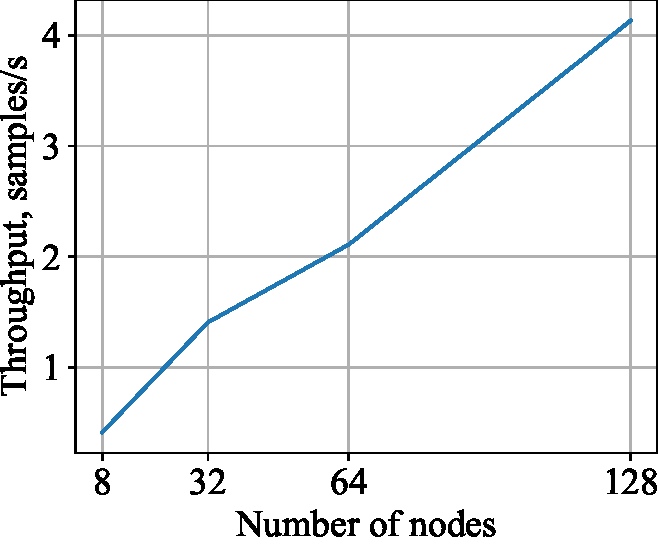
\includegraphics[width=0.7\linewidth]{resources/scaling_t4.pdf}
    \caption{Scaling of SWARM parallelism throughput with the number of nodes.}
    \label{fig:scaling_t4}
\end{figure}


Figure~\ref{fig:scaling_t4} shows the results of our evaluation. It can be seen that the training performance exhibits an approximately linear scaling pattern, which can be explained by the high efficiency of both the stochastic wiring strategy and the auxiliary training components such as the DHT and the All-Reduce protocol used for gradient averaging.

\section{Compression-Aware Architectures}\label{appendix:compression}

Since pipeline parallelism has several distinct points of communication, the network overhead can be reduced considerably by reducing the size of data at these communication points. To exploit this, we develop compression-aware architectures that apply extreme compression at these points. We study two distinct communication bottleneck layers: (1) compression through a linear bottleneck layer, and (2) compression through a bottleneck induced by the maxout activation function~\citep{goodfellow2013maxout}. We also study how compressing the activations and gradients at the communication points to 8 bits affects the predictive performance.

\subsection{Description}\label{appendix:compression_detailed}

\paragraph{Fully connected layers (baseline):} Fully connected layers in models such as Transformers consist of a multilayer perceptron with a single hidden layer and a nonlinear activation function. Without biases and with a residual connection~\citep{resnet} from the inputs to the outputs, this can be described as $\text{MLP}(\mathbf{x}, \mathbf{w}_1, \mathbf{w}_2) = \sigma(\mathbf{x}\mathbf{w}_1)\mathbf{w}_2 + \mathbf{x}$,
where $\mathbf{x}\in\mathbb{R}^{b\times s\times m}$, $\mathbf{w}_1\in\mathbb{R}^{m\times h}$, $\mathbf{w}_2\in\mathbb{R}T^{h\times m}$, and $\sigma(\cdot)$ is a nonlinear activation function such as ReLU~\citep{alexnet}; $b$, $s$, $m$, and $h$ are the batch, sequence, model, and hidden dimensions of the neural network. To compress the output of the MLP layer, we want to apply a compression layer between two consecutive stages. For example, if we have 24 layers and 4 stages, we need 3 compression layers at layers 6, 12, and 18.%

\paragraph{Quantized activations:} A natural way to reduce the communication intensity is to send activations and gradients with respect to activations in reduced precision. However, simply casting tensors to a lower precision may slow down convergence and cause instabilities. Instead, we use dynamic 8-bit quantization with blockwise scaling from~\citep{adam8bit}. This technique reduces communication by ${\approx} 2$x and ${\approx} 4$x for half and full precision, respectively.

On the other hand, quantizing and dequantizing activations can add compute overhead on every microbatch processed. Our implementation circumvents that overhead by performing quantization asynchronously on the CPU. However, this is not required, as blockwise (de)quantization takes less than 1\% of total computation time: see Appendix~\ref{appendix:time_to_solution} for details.


\paragraph{Bottleneck layers:} We experiment with simple bottleneck layers that work by compressing the output features of the MLP by linear projection:
\begin{gather*}
    \text{Bottleneck}(\mathbf{x}, \mathbf{w}_1, \mathbf{w}_2, \mathbf{w}_c, \mathbf{w}_d) = \\ 
    = \text{LayerNorm}(\text{LayerNorm}(\text{MLP}(\mathbf{x}, \mathbf{w}_1, \mathbf{w}_2))\mathbf{w}_c)\mathbf{w_d},
\end{gather*}

where $\mathbf{w}_c\in\mathbb{R}^{m\times c}$, $\mathbf{w}_d\in\mathbb{R}^{c\times m}$ are compression and decompression parameters with compression dimension $c<m$. We find it critical to use layer normalization \cite{ba2016layernorm} to ensure training without divergence. The parameter matrix $\mathbf{w}_c$ resides in one stage and its outputs are transferred to the next stage that holds the parameters $\mathbf{w}_d$, which requires $m/c$ times less communication compared to the original model. Note that adding a bottleneck only adds two linear layers for the forward pass and decreases the size of MLP activations; thus, its computational overhead is negligible (less than 1\% for typical sizes, see Appendix~\ref{appendix:time_to_solution}).

\paragraph{Maxout compression:} Compared to bottleneck compression, maxout compression works by using the maxout activation function~\citep{goodfellow2013maxout} for compression rather than a linear projection. The maxout function of factor $k$ takes inputs with a hidden dimension of $d$ and reduces this dimension by a factor of $k$ by computing the maximum value for each non-overlapping window of $k$ features. We use maxout compression as follows:
\begin{gather*}
    \text{Maxout}(\mathbf{x}, \mathbf{w}_1, \mathbf{w}_2, \mathbf{w}_d) = \\ \text{LayerNorm}(\text{maxout}_k(\text{LayerNorm}(\text{MLP}(\mathbf{x}, \mathbf{w}_1, \mathbf{w}_2))))\mathbf{w_d},
\end{gather*}

where the output is reduced by a factor of $k$ through the maxout function in the previous stage, and then sent to the next stage which holds the decompression matrix $\mathbf{w}_d{\in}\mathbb{R}^{m/k\times m}$.

    \begin{table*}[h!]
    \centering
    \captionof{table}{Performance of compression methods for a Transformer language model with adaptive inputs on WikiText-103. The asterisk denotes that the difference is not statistically significant.}
    \label{tab:steps_to_22}
    \begin{tabular}{@{}lccccc@{}}
    \toprule
    \multirowcell{2}[-0.5ex][l]{Method} & \multirowcell{2}[-0.5ex]{Ppl after\\ 286K steps} & \multirowcell{2}[-0.5ex]{Steps to\\ppl 22} & \multirowcell{2}[-0.5ex]{Data\\ transfer} & \multicolumn{2}{c}{Extra compute} \\ \cmidrule(l){5-6} 
     & &  &  & Absolute & Relative \\ \midrule
    No compression & 21.02 & 1x & 1x & 0 & None \\
    8-bit compression & 21.13 & $\text{0.97x}^{*}$ & 0.5x & 1.2ms & None \tiny{(overlapped)} \\
    Bottleneck & 21.76 & 1.26x & 0.5x & 1.96ms & $\leq 1\%$ \\
    Maxout & 21.83 & 1.28x & 0.5x & 2.04ms & $\leq 1\%$ \\ \bottomrule
    \end{tabular}
    \end{table*}

\subsection{Evaluating the Speed-Quality Tradeoff}
\label{appendix:compression_tradeoff}

While compression techniques reduce the communication overhead, they might also degrade the perplexity reached in a certain time and the final perplexity after a specific number of steps. To study these tradeoffs, we train a Transformer language model with adaptive inputs~\citep{baevski2019adaptiveinputs} on the WikiText-103 dataset and measure how compression-aware architecture variants affect convergence.

Our setup follows that of~\citep{baevski2019adaptiveinputs} with one difference: we use a sequence length of 2048 instead of 3072 to fit this model into our smaller GPUs.
To measure the time to solution, we look at the number of iterations it takes to converge to the training perplexity of \textbf{22}. We evaluate the baseline model and three compression-aware modifications from Section~\ref{appendix:compression_detailed}: bottleneck, maxout, and block-wise dynamic 8-bit quantization, each with 2 pipeline stages and each a compression factor of 2x.

The results can be seen in Table~\ref{tab:steps_to_22}. We can see that 8-bit compression does not degrade the time to 22 perplexity and maintains close to the final perplexity of the baseline. The compression-aware bottleneck and maxout architectures perform equal to each other, but degrade final perplexity slightly and increase time to a perplexity of 22 by 26--28\%.

Using these results, one can determine which method is optimal for their hardware setup. For instance, training with maxout with 2 pipeline stages needs $28\%$ more steps, but accelerates the communication phase by $2$x. If communication is the limiting factor, using maxout or bottleneck compression layers will offer {\it improved} time to perplexity despite the performance degradation. However, the same two techniques would result in slower training in a setup where network bandwidth is unlimited.

In turn, 8-bit quantization reduces communication cost without slowing down per-iteration convergence, making it a ``safe bet'' for situations where the per-iteration convergence must be preserved.
In our large-scale experiments (Section~\ref{sect:experiments_large}), we opt to using quantization since it was enough to fully saturate the GPUs.
If network bandwidth is still a limiting factor, one can combine quantization with bottleneck or maxout compression to further reduce communication.

\vspace{-6pt}
\subsection{Additional Experiments}\label{appendix:compression_extra}

The additional experiments in this section have two purposes: (1) to evaluate how compression methods vary with the number of stages and (2) to evaluate an additional setting that is closer to modern pretraining setups such as GPT-2/3.

While (1) has further implications for scaling, (2) is helpful to account for confounding factors that might have been overlooked in the main experiments on WikiText-103. The WikiText-103 baseline uses non-BPE vocabulary, a long sequence length, and uses adaptive inputs \citep{baevski2019adaptiveinputs}, all of which are not frequently used in modern pretrained Transformers since GPT-2 \citep{radford2019language}.

\begin{table*}
\centering
\caption{Results of language models trained on the OpenWebText Corpus (OWT). The baseline model has 253M parameters and is trained for 8 GPU-days. We apply bottleneck and maxout compression to our baseline in 2 and 4 stages with a compression factor between 2--4x. PTB=Penn Treebank, 1BW=Billion word corpus.}
\label{tab:compression}
\begin{tabular}{lcccccccc}\toprule
                &        &             & \multicolumn{6}{c}{Validation perplexity}                        \\ \cmidrule{4-9} 
Model                &  Stages & Compression & OWT & LAMBADA & WikiText-2 & WikiText-103 & PTB    & 1BW   \\\midrule
Baseline        &   --      & -- &   19.7     &  86.4     &    56.2   &    35.4    &  133.0   &   80.9   \\\midrule
8-bit Quantization  &  2      & 2x        &     19.6       &   89.1     &    {\bf 56.0    }  & {\bf   35.0 }        &  132.7   &  79.8    \\
Bottleneck        &   2      & 2x        &   {\bf19.5  }      &  87.7 &     56.5      &    35.2  &  {129.8 }   &   79.2   \\
Maxout  &  2      & 2x        &     19.6       &  {\bf 85.4 }     &     56.6      &   35.2        &  {\bf 126.8 }    &  {\bf78.8  }   \\\midrule
8-bit Quantization  &  4      & 2x        &    {\bf 19.7  }     & {\bf  87.9  }   &    {\bf 56.3    }  & {\bf   35.2 }        &  {\bf133.9 }  &  {\bf79.8}    \\
Bottleneck         &  4      & 2x       &   21.7          &   100.0      &   66.4   &    40.0   &  149.6      &     89.5  \\
Maxout            &  4      & 2x       &  21.4           &  { 89.9  }    & {  63.9 }      &  {     39.5}      & {142.1   }    &   {86.2 }   \\\midrule
Bottleneck        &   2      & 4x        &   21.6          &    99.8     &   64.8        &   39.6          &  145.6      &   88.3    \\
Maxout            &   2      & 4x        & {\bf20.5}      &  {\bf 89.6 }     &   {\bf  60.0}      & {\bf    37.1 }       & {\bf 141.7 }     &  {\bf83.5}     \\\midrule
Bottleneck      & 4  &  4x   &  28.9  &   141.6      &  100.2 &  58.1  &   235.5     &   118.3    \\
Maxout            &  4      & 4x       &   {\bf 21.3} &   {\bf 93.5 }    &  {\bf 63.6  }      & {\bf 39.2}           &   {\bf 147.7 }   & {\bf 89.1  } \\\bottomrule   
\end{tabular}%
\end{table*}

\vspace{-6pt}
\paragraph{Experimental setup:}

As a baseline, we train a Transformer language model~\citep{transformer} on the OpenWebText corpus~\citep{gokaslan2019openwebtext}. We use the following hyperparameters: sequence size 512, 16 layers with model dimension 1024, and hidden dimension 4096 for a total of 253M parameters. We use byte pair encoding~\citep{sennrich-etal-2016-neural,radford2019language} with a vocabulary size of 50264 symbols. We do not use dropout or other regularization, since our models underfit. We run these experiments in Fairseq~\citep{Ott2019fairseqAF}.

We test bottleneck and maxout compression for a compression factor of 50\% and 75\% compared to the original size over two and four stages. We look at how using these compression-aware architectures affects the performance compared to the compression that they achieve.
\vspace{-6pt}

\paragraph{Results:} The results of our compression-aware architectures are shown in Table~\ref{tab:compression}. We can see that while the bottleneck architecture is competitive with maxout for a compression factor of 2x with two stages, maxout has better perplexities if more stages or a higher compression ratio is used. The out-of-distribution perplexities vary consistently with the in-distribution perplexity, which suggests compression-aware architectures do not degrade the out-of-distribution performance more than the in-distribution performance. As such, the maxout compression is an effective technique to reduce the bandwidth requirements of pipeline parallel training further.

While the 8-bit blockwise quantization can only compress the activations by a factor of two (16-bit $\rightarrow$ 8-bit), it does not affect the quality as much when compared to the baseline. As such, the 8-bit quantization appears to be a reliable default choice to reduce the communication overhead for pipeline parallelism.

When considered together with the square-cube law for distributed training and SWARM parallelism, compression-aware architectures allow for better scaling of large neural networks trained over preemptible low-bandwidth peers. Thus, compression-aware architectures improve the accessibility and affordability of training large models outside HPC environments.

\vspace{-6pt}

\section{Time To Solution}\label{appendix:time_to_solution}

In this section, we evaluate the compression-aware techniques proposed in Appendix~\ref{appendix:compression_detailed} from a practitioner's point of view. A natural way to compare these techniques is in terms of ``the time to solution'', i.e., the wall-clock time it takes to achieve the desired validation objective.
In practice, this time depends on three main factors: the compression strategy, the distributed training algorithm, and the computational infrastructure.

In order to disentangle these factors, we first address the relationship between the training algorithm and the infrastructure.
As we discuss in Section~\ref{sect:method_swarm} (and later in Appendix~\ref{appendix:equivalence}), SWARM parallelism has the same per-iteration behavior as other synchronous methods. Theoretically, the choice of an optimal training system should come down to whichever algorithm has the highest training throughput.




To verify this argument in practice, we compare the per-iteration and per-hour performance of SWARM against fully synchronous training. For this experiment, we train the ALBERT model~\citep{albert} on the WikiText-103 dataset~\citep{wikitext103}. We use the ALBERT-Large architecture with 4 layer groups that correspond to 4 SWARM stages \textit{without the architecture modifications from Appendix~\ref{appendix:compression}}. We follow the exact hyperparameters from the original paper: for example, we use the LAMB optimizer~\citep{lamb} with the batch size of 4096 and the sequence length of 512. We train this model in three setups: traditional distributed training with 8 V100 workers, SWARM with 8 preemptible V100 GPUs, and SWARM with 32 preemptible T4 workers.

\begin{table}[t]
\centering
\captionof{table}{Training time and costs.}
\label{tab:cost}
\begin{tabular}{@{}lccc@{}}
\toprule
\multirowcell{2}[-0.5ex][l]{Setup} & \multirowcell{2}[-0.5ex]{Time, hours} & \multicolumn{2}{c}{Cost, \$} \\
\cmidrule(lr){3-4} 
    & & Hourly & Total \\
\midrule
$8\times V100$, reliable         &175.4&7.834&1374\\
\midrule
$8\times V100$, preemptible           &192.6&5.383&1037\\
\midrule
$32 \times T4$, preemptible           &140.8&3.536&497.8\\
\bottomrule
\end{tabular}
\end{table}

To quantify the time to solution, we measure the wall time required to achieve the ALBERT objective equal to \textbf{1.5}. Additionally, we report the per-hour cost of each experimental setup and the total cost of achieving a loss of 1.5 using public cloud provider pricing estimates in \cref{tab:cost}.

Figure~\ref{fig:convergence_iterations} demonstrates that SWARM matches the per-iteration learning curves of traditional distributed training (PyTorch DistributedDataParallel) up to the variation comparable to caused by changing the random seed. However, SWARM parallelism can achieve the loss of 1.5 more cost-efficiently and faster by using preemptible instances. In turn, \textit{when forced to use homogeneous and reliable GPUs}, SWARM would have slightly inferior performance compared to conventional algorithms, which was first demonstrated in Section~\ref{appendix:training_throughput}.

\begin{figure}
\centering
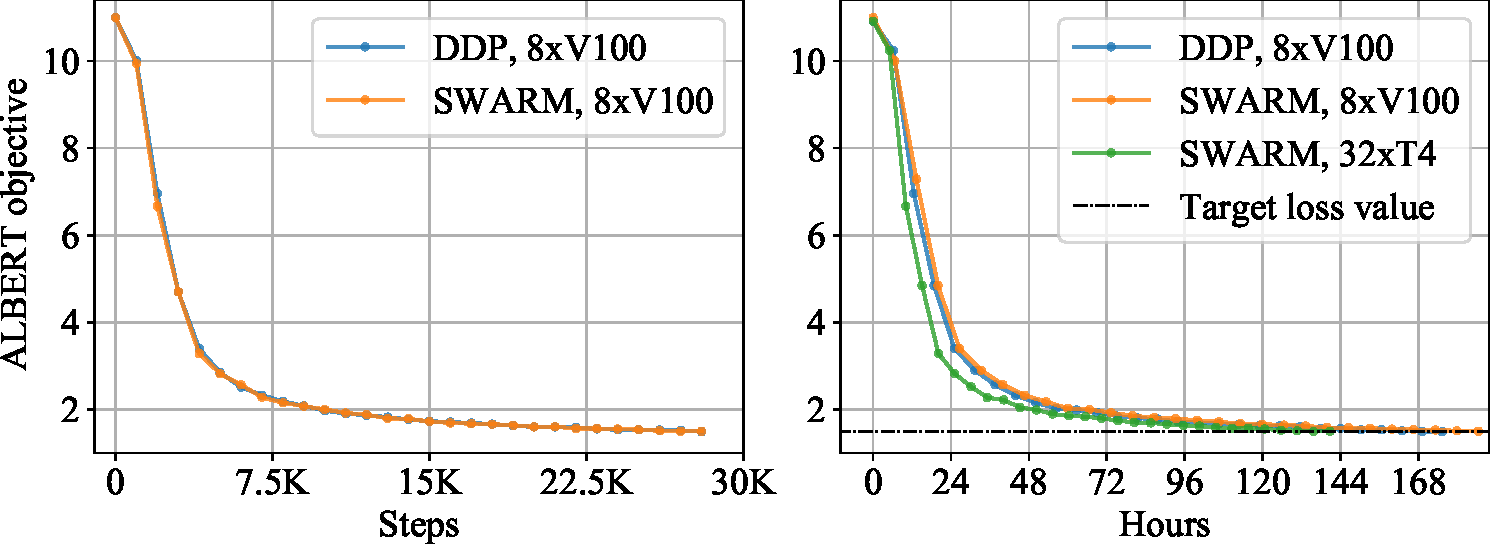
\includegraphics[width=\linewidth]{resources/albert_learning_curves.pdf}
\captionof{figure}{Convergence curves of ALBERT with SWARM and standard data-parallel training.}
\label{fig:convergence_iterations}
\end{figure}




% \clearpage\section*{\Large Supplementary Materials - DGR-MIL: Exploring Diverse Global Representation in Multiple Instance Learning for Whole Slide Image Classification}







\end{document}
